
% !TeX program = xelatex

%使用hustthesis这个模板。
% draft版本的正文页包括页眉(“华中科技大学xx学位论文”)、页眉修饰线(双线)、页脚(页码)和页脚修饰线(单线)。
% final版本的正文页不包括页眉、页眉修饰线和页脚修饰线,仅包 含页脚(页码)。如果不指定,默认设置为final。

% degree用来指定论文的种类
% language用来指定论文语言。特别的,如果设定为english-draft,将会剔除论文中的所有中文内容,这有利于在未安装中文字体的环境中使用。如果不指定,默认设置为 chinese。


\documentclass[format=draft,language=chinese,degree=master]{hustthesis}
%\documentclass[format=final,language=chinese,degree=master]{hustthesis}

%\setcounter{tocdepth}{2} %设置目录的层级

%使用下面的这两个宏包来生成带书签和超链接的PDF文件。
%\usepackage[bookmarks,bookmarksopen,bookmarksdepth=2]{hyperref}
%\usepackage[pdftex,CJKbookmarks=true,colorlinks=true]{hyperref} %LaTeX Error: Option clash for package hyperref
\usepackage{indentfirst}

\stuno{M201672905}
\schoolcode{10487}
\title{基于Vxworks的调试通道的\\
设计与实现}{A design and implementation of debug channel based on Vxworks.}
\author{郑松}{Song Zheng}
\major{计算机应用技术}{Computer Applications Technology}
\supervisor{张杰\hspace{1em}讲师}{ Lecturer Jie Zhang}
\date{2018}{5}{27}
%\date{\today}

\zhabstract{
	在嵌入式软件的开发、移植、运行时都需要输出一些调试或日志信息,目前VxWorks当中使用WorkBench集成开发平台来完成软件的开发、调试工作,它的调试工具使用的是一种典型的在线调试方式,但是在我们项目的实际生产环境中希望能够使用一种离线的调试日志的方式来进行程序的调试工作,他们希望在设备运行的大量应用程序当中加入调试信息,这些调试信息都能够自动的传输到普通的PC上,之后他们可以查看这些调试信息,对这些信息进行分析。
	

	本文从项目的实际需求出发,详细地了解了他们所使用的设备的情况和具体的需求,给出了一个总体的设计方案,由于目前大多数的设备都已不再将RS-232的串口作为必须的标准接口,而是大量的使用USB接口,在项目所处的实际环境当中也没有可供使用的串口,因此在调试信息的传输过程中只能够使用USB接口,本设计即以USB转串口驱动为基础,并配以我们设计的调试接口组成一个实际可用的调试通道,方便它们在程序的开发和移植的过程中进行离线的调试。
	
	根据我们的方案需求,我们分析了VxWorks下的设备驱动所需的关键技术,然后在VxWorks下设计出了一个特定需求的USB转串口的驱动程序和一个普通的USB转串口驱动程序,驱动程序具有双向缓冲功能,同时具有即插即用、使用方便等特点。	
	然后我们给上层需要输出调试信息的应用设计了两个调试接口。一个Log调试接口,我们为这个接口设计了一个自定义的调试通道的传输协议;另外我们也给出了一个标准输出重定向的调试接口,方便开发人员直接使用标准输出进行调试信息的输出。	 
	最后我们通过对系统的整体测试和对各个部分分别进行测试,验证了本次的调试通道设计基本完成,系统运行可靠,满足所需完成的要求。

}
\zhkeywords{VxWorks操作系统,设备驱动开发,调试,USB转串口}

\enabstract
{
    In the development, migration, and runtime of embedded software, some debugging or log information needs to be output. At present, Workbench integrated development platform is used in VxWorks to complete software development and debugging. Its debugging tool uses a typical online debugging. The way, but in the actual production environment of our project, we hope to use an offline debug log to debug the program. They want to add debugging information to a large number of applications running on the device. These debugging information can be automatic. It is transmitted to a normal PC, after which they can view the debug information and analyze the information.

This article starts from the actual needs of the project, understands in detail the conditions and specific requirements of the equipment they use, and gives an overall design proposal. Since most of the current devices no longer use RS-232 serial ports as The necessary standard interface, but a large number of use of the USB interface, there is no serial port available for use in the actual environment of the project, so only the USB interface can be used during the transmission of debugging information, this design is to USB to serial port Based on the driver, and equipped with the debugging interface we designed to form a practical and available debugging channel, they are convenient for offline debugging during program development and porting.

According to our solution requirements, we analyzed the key technologies needed for device drivers under VxWorks, and then designed a specific USB-to-serial driver and a generic USB to serial driver under VxWorks. Two-way buffer function, with plug and play, easy to use and so on.
Then we design two debugging interfaces for the application that needs to output debugging information. A Log debug interface, we have designed a custom debug channel transfer protocol for this interface; in addition we also provide a standard output redirection debug interface to facilitate developers to directly use the standard output for debugging information output.
Finally, we test the whole system and test each part separately to verify that the debug channel design is basically completed, the system is running reliably, and the required requirements are fulfilled.

}
\enkeywords
{VxWorks operating system, device driver development,debugging, USB to serial}

\begin{document}
% frontmatter用于设定论文的状态、改变样式,其具体使用见简单示例。 
% frontmatter用在文档最开始,表明文档的前言部分(如封面,摘要,目录等)的开 始。
\frontmatter

% maketitle的作用和makecover的作用相同,用于生成封面和版权页面
\maketitle


% makeabtract用于生成中英文的摘要页面。
\makeabstract

% tableofcontents用于生成目录
\tableofcontents

% listoffigures 和 listoftables 分别用于生成图片和表格索引,可以根据要求在论文的前言中使用或者是在附录中使用
%\listoffigures
%\listoftables

% mainmatter表示论文正文的开始。
\mainmatter

\clearpage
\chapter{绪论}
\section{课题背景以及来源}
	嵌入式系统目前不断发展和壮大,使用嵌入式的场景越来越多,同时对嵌入式系统进行软件开发和移植工作也越来越多,由于每种嵌入式系统都有不同的软件接口和特性。所以在不同的嵌入式系统上进行软件开发和移植工作要根据其特性使用不同的方法,在我们所熟悉的通用操作系统(Linux、Windows、MacOS)下进行软件设计和开发时它们通常都会有现成的集成开发环境和调试工具。
	然而在嵌入式软件的开发和移植过程当中,由于嵌入式设备所独有的特点,对嵌入式系统上的软件的调试、分析一直是一个费时费力的工作。在整个的嵌入式的开发过程当中软件的调试占据了软件开发周期中的大部分时间。这是因为在设计软件时难免会出现各种各样的错误,这些错误可能需要进过反复的修改才能够达到设计的要求。因此一个好的调试、分析工具可以给嵌入式软件开发人员带来很大的帮助,使其达到事半功倍的效果,快速完成软件开发过程中的调试、分析,软件运行过程中调试信息的定位等工作。
	
	VxWorks因为其可靠性和实时性被广泛地应用对系统的实时性要求很高的领域当中,如:通信、航天、军事等\cite{刘小军2008基于},在进行VxWorks应用程序的开发或者是将Linux下的应用程序移植到VxWorks中时都需要在程序中加入大量的调试信息,在程序的正常运行当中也需要输出一些日志信息,方便之后对程序运行过程中产生的问题进行具体的分析。目前VxWorks当中使用WorkBench集成开发平台来完成软件的开发、调试工作,这是一种典型的在线调试方式\cite{陈洋2007VxWorks}\cite{张鹏2007基于},但是在中船重工的实际生产环境当中他们希望使用一种离线的调试日志的方式来进行程序的调试工作,它们希望在设备运行的大量应用程序当中加入调试信息,这些调试信息都能够自动的传输到普通的PC上,他们能够在之后查看其调试信息,对这些信息分析工作。并且通常对于宿主机和目标机之间的传输都是通过网口或者串口,然而目前的大多设备都已不再将RS-232的串口作为必须的标准接口,而是大量的使用USB接口,嵌入式设备上又大多没有配备网口的需求,因此在调试信息的传输过程中只能够使用USB接口。
	
	本次基于VxWorks的调试通道的设计来源于中船重工的实际需求,我们基于VxWorks开发出一个小巧易用的调试信息的传输通道,方便它们将应用程序的调试信息传输出来,以进行一个事后的分析工作,对于底层的信息传输我们使用USB转串口来实现,USB转串口的转换器使用CP2102模块来实现,并在此基础上设计了给应用层使用的调试接口。
	
			
\section{国内外概况}
	
	在嵌入式系统上由于其资源有限,所以在嵌入式系统上的调试必须采用交叉调试的方式。用户无法直接在嵌入式系统平台上调试被调试的程序,因此必须要借助于宿主机上丰富的调试资源通过一定的调试通道配合目标机共同完成对被调试程序执行状态的实时跟踪,从而快速有效地对程序错误进行定位,纠正错误,提高调试速率和软件质量。
	
	目前嵌入式系统上主要使用三类的调试技术进行调试。

	
	\textbf{1. 目标监控程序调试技术}
	
	目标监控程序调试技术是在目标机中植入一段特殊的代码即监控程序来实现对目标机的调试控制宿主机和目标机之间可以仅仅通过通过简单的通讯设备(如网口,串口等进行连接),不需要额外的硬件开销,同时在目标机上也不需要特殊的硬件支持。目标监控程序调试技术又可以根据监控程序的实现方式不同而分为两种:一种是作为一个独立的程序运行在目标机上,如GDBServer,ROM Monitor,这种方式下的监控程序主要是作为一个操作系统上的应用程序用于用户用户应用程序的调试。若要实现对操作系统进行调试,则需要同时具备完成简单的硬件初始化、下载以及调试被调试程序的功能;开发难度较大。另外一种是监控程序编译进操作系统镜像之后一起在目标机上运行,如GDB Stub、VxWorks的target agent、Windows CE的KITL调试技术等等,这种监控方式可以直接调用操作系统中的可用代码(如设备驱动),减少代码的开发量,还可以方便的进行接口功能扩展,丰富调试通道,解决了接口资源受限目标机的调试问题,同时监控程序一般都可以同时用于操作系统以及用户应用程序的调试。
	
	\textbf{2. 片上调试技术}
	
	片上调试技术是随着芯片技术发展特别是处理器的封装越来越表贴化,加大了ICE的仿真探头开发难度的情况下发展起来的,是通过在目标机处理内部集成调试模块来接管被调试程序的运行控制完成调试操作的。
	片上调试技术使用两级模式:运行模式和调试模式,在调试模式下通过目标机上的提供的调试端口同宿主机交互信息完成调试功能。根据芯片调试接口支持不同,常用的片上调试技术包括:BDM调试技术。BDM也叫后天调试适配器。BDM调试是利用处理器内部提供的BDM,增加一个可以插入后台模式指令激活后台处理的串行口作为在线仿真接口,在定义的执行点上,由在线仿真器将后台调试指令覆盖在原代码上,控制目标处理器的运行和停止。
	
	
	\textbf{3. 利用打印信息进行调试}\\
	利用打印信息进行调试是最一般的调试技术,这种技术也称为监视,只需要应用程序内部适当的地方加上printf调用即可。这样就可以完成对应用程序中相关变量的监视工作,进而推断出错误所在。这种调试方式简单方便,不需要复杂的设置,但是缺点是获取到的信息有限且不能进行断点设置,单步执行等操作。
		
	
	
	在这些调试技术领域中,宿主机和目标机之间的通信方式主要有串口方式、以太网接口,大多数的远程调试中使用的是串口传输方式,但是串口通信存在着速度慢、通信距离受限等弊端,而以太网口的传输方式则可以克服串口方式的不足,不仅可以提供稳定可靠的数据传输,而且无论是传输速度还是传输距离都远远优于串口方式,是一种快速高效的通信方式,但是网络传输需要网络芯片的支持,而很多的嵌入式设备并没有这种需求,所以很所设备上无法实现网络传输的范式来进行调试,目前USB已经成为嵌入式平台的通用接口,使用USB做为传输方式已经广泛的应用在嵌入式系统的开发当中,逐渐替代了RS-232接口,USB不仅可以实现直接传输,还可以使用CDC协议虚拟成其他通信设备进行传输,USB在调试技术方面的使用也有相关的研究,如GDB中的USB Network调试的实现,但是USB应用在这方面的资料相对较少,因此对其进行研究与实现具有重要的意义。

	
	对于USB口转串口的转换器,国内外通常都会采用两种方案:一种是以CY7C68013芯片为代表,自己从底层的硬件和固件开始,进行彻底而全面的系统开发,这种方案的成本和开发难度都很大,通常都不会使用这种方案。另外一个方案是采用类似于CP2102等专用的双向USB口转串口芯片来进行设计,这种方案简单实用,只需要对芯片的功能进行了解和应用即可,无需深入开发\cite{Yao2009Design}\cite{Zhou2002The}。因此我们在此会选择CP2102芯片来进行调试通道的设计。	


	
	

\section{论文的主要工作和组织结构}	
	主要工作:在嵌入式实时操作系统VxWorks上实现一个能够满足程序的调试信息输出的通道,主要包括两个部分:一个将USB总线技术和RS-232接口相结合,设计出一个满足特定要求的、实用的USB转串口驱动程序;另一个是设计给应用层调用的日志传输接口封装程序和标准输出重定向接口封装程序。\\
 本文共分为六章来进行描述,对每一个章节我们做了如下的安排:
 
 第一章为绪论部分,主要描述了本次的课题的背景和来源、国内外的发展状况以及本文的结构安排。
 
 第二章介绍了首先介绍对于我们的调试通道的总体设计,然后介绍了调试通道的开发所需要了解的系统知识和关键技术,主要包括VxWorks系统及驱动开发的知识、USB技术相关知识。
 
 第三章介绍了USB口转串口驱动程序的设计和实现,包括驱动程序程序当中对于缓冲区和信号量的设计,我们使用CP2102模块开发和VxWorks下的USB开发的内容,然后给出了USB口转串口驱动的具体实现,包括特定需求下的单设备驱动和多设备支持的驱动
 
 第四章主要介绍了应用层的接口封装部分,主要包括Log接口的设计,标准输出重定向接口的设计,以及PC客户端的协议解析部分。
 
 第五章主要内容是系统的功能测试部分,我们进行了整体测试和各个部分的功能测试。
 
 最后在结束语部分对整个的工作进行了总结,指出了本次的工作的不足之处,并对下一步的工作进行了展望。 



\clearpage
\chapter{调试通道总体设计与关键技术}

\section{总体设计}
	在嵌入式软件的开发、移植、运行时都需要输出一些调试或日志信息,目前VxWorks当中使用WorkBench集成开发平台来完成软件的开发、调试工作,它所使用的调试方式是一种典型的在线调试方式,但是在项目的实际生产环境当中他们希望使用一种离线的调试日志的方式来进行程序的调试工作,它们希望在设备运行的大量应用程序当中加入调试信息,这些程序的调试信息都能够自动的传输到普通的PC上,他们能够在之后查看其调试信息,对这些信息分析工作。
	
	基于以上的需求,此次我们的工作就是在VxWorks下完成一个能够满足他们的需求的调试通道,在主机端我们使用一个分析程序来对目标机上传输过来的调试数据进行分析;在目标机端我们给应用程序提供一个调试接口,将调试信息从通信接口中传输出去,本次设计的调试通道主要应用于VxWorks下程序移植时大量调试信息的输出的场景。对于在该应用场景下的整个调试通道的框架如\autoref{fig:sys-data-diagram}所示。

\begin{figure}[!h]
\centering
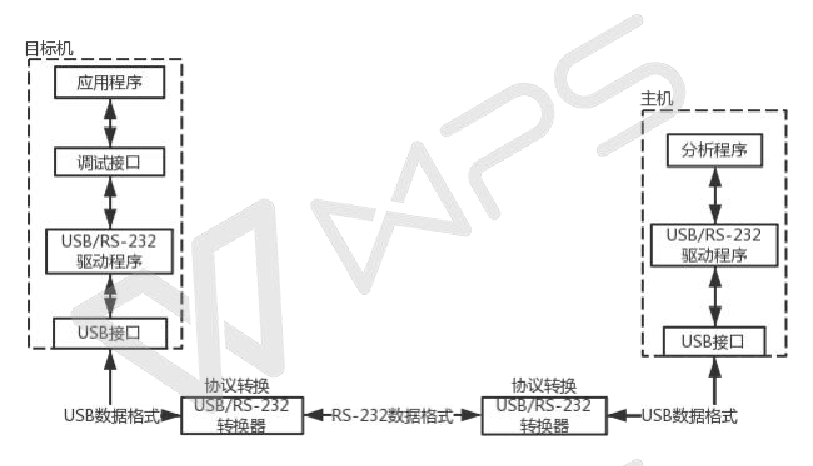
\includegraphics[width=1.0\textwidth]{./graphics/sys-data-diagram.pdf}
\caption{调试通道框架图}\label{fig:sys-data-diagram}
\end{figure}

	在我们所设计的调试通道当中,目标机上的上层应用程序会调用调试通道中所提供的调试接口,通过调试接口将调试信息传递给通信接口,由于设备上没有可用的RS-232串口,而USB的体系结构又是主从式的,无法直接作为调试通道的通信接口来使用,为了解决这个问题,在我们的调试通道当中使用外部的USB/RS-232的转换器来实现通信接口,同时在系统上使用与设备相对应的USB/RS-232设备驱动程序。这样PC端的应用软件应用软件仍然是针对RS-232串行端口编程的,外设也是以RS-232为数据通信通道的,但是PC端到外设之间的物理连接却是USB总线,其上的数据格式也是USB数据格式。
	
	在VXWorks中并没有现成可用的USB转串口驱动以及USB转串口转换器,所以我们需要自己选择一个外部的USB/RS-232转换器,以及针对该USB/RS-232转换器的USB转串口驱动。在主机端都会有已经实现好的USB转串口驱动程序,我们只需要提供转换器即可,这样用户在不需要理会USB的复杂的内部协议的情况下来享受USB接口的即插即用、数据可靠传输、扩展方便等优点。分析程序会自动接收串口的数据,完成协议分析、调试信息的定位等工作。
\begin{figure}[!h]
\centering
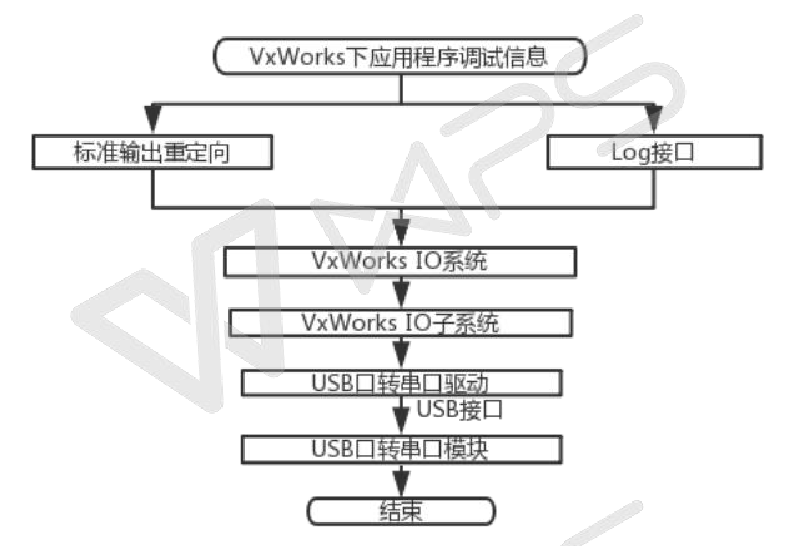
\includegraphics[width=1.0\textwidth]{./graphics/debug-system-diagram.pdf}
\caption{目标机调试通道层次结构图}\label{fig:debug-system-diagram}
\end{figure}
	
	对于目标机上的调试通道的结构如\autoref{fig:debug-system-diagram}所示。在VxWorks当中I/O 系统和I/O子系统是作为操作系统的重要组成部分已经实现好了的,我们的调试通道所需要设计的部分主要是接口模块和USB口转串口模块。
	
	提供给应用层的接口模块负责将系统应用层的输出通过我们的USB口转串口驱动程序传输到windows PC机,输出的形式包括特定内容的格式化的输出和普通的重定向的输出,格式化的输出我们会使用自定义的Log接口进行格式控制,为此我们设计了一个自定义的Log协议格式,其中的内容包含有调试级别、调试信息所在的文件、调试信息所处的行号、输出该条调试信息的时间等;重定向的输出包括RTP模式下的重定向和task模式下的重定向,VxWorks中对于这两种模式需要使用不同的重定向方式。
	
	USB口转串口模块用于在VxWorks上实现一个USB口转串口驱动程序,负责将上层应用的信息传输到windows PC,包括一个特定需求的驱动程序的实现和一个普通的驱动程序的实现。对于本次特殊需求的驱动程序相对于普通的驱动程序而言在流程和结构上进行了修改,以使其达到特定的要求,具体的实现我们会在第三节进行介绍。两种实现方式中都会包含有驱动程序加载、卸载模块,设备的打开、关闭、读、写、控制模块。同时在驱动程序中还需要一个数据的管理模块,我们会使用循环缓冲区来管理数据。


	


\section{关键技术}

\subsection{VxWorks驱动开发}
	
	在VxWorks当中使用I/O子系统来管理设备驱动,I/O 子系统在整个VxWorks当中起着承上启下的作用,各种类型的设备都必须要向I/O子系统进行注册才能够被内核访问,I/O子系统在VxWorks当中的作用是维护系统设备表、系统驱动表、系统文件描述符表\cite{VxWorks内核解读}\cite{曹桂平2011VxWorks}。设备驱动在VxWorks中就靠这三个数据结构来进行管理,所以对于设备驱动而言非常重要。设备驱动程序初始化时会对硬件完成初始化的配置,同时会向I/O子系统注册自己,注册之后I/O子系统才能找到该驱动。

\noindent \textbf{1. 系统设备表}

	系统设备表是VxWorks中为了管理系统上的所有设备而使用的一个链表,系统设备表中每一个节点都是一个DEV\_ HDR类型的结构体,系统会将每个设备DEV\_ HDR连接在如\autoref{fig:VxWorks系统设备示意图}所示的系统设备表中。DEV\_ HDR是wind内核规定的每一个设备都必须要具有的一个数据结构,且必须是设备自定义结构的第一个成员,之后系统只会使用这个结构来代表该设备。DEV\_ HDR结构体当中只包含有三个成员:一个设备链表节点;一个设备驱动号;一个指向设备名的指针。
	其定义如\autoref{fig:DEVHDR} 所示。

\begin{figure}[!h]
\centering
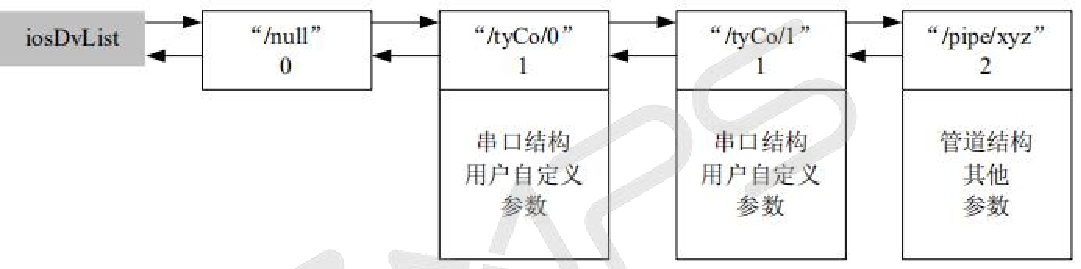
\includegraphics[width=1.0\textwidth]{./graphics/vxworks-device-link.pdf}
\caption{VxWorks系统设备示意图}\label{fig:VxWorks系统设备示意图}
\end{figure}
	
\begin{figure}[!h]
\centering
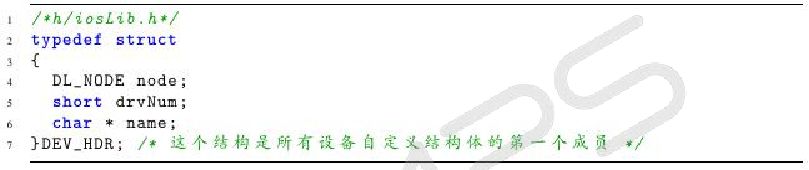
\includegraphics[width=1.0\textwidth]{./graphics/DEVHDR.pdf}
\caption{DEV\_ HDR结构体}\label{fig:DEVHDR}
\end{figure}

同时VxWorks系统提供了一个设备的注册函数iosDevAdd( DEV\_ HDR *pDevHdr, char *name, int drvnum),该函数用来将一个设备添加到系统设备表当中,系统设备表在每次添加设备时就会在表中增加一个节点表示该设备,删除设备时就会将该设备的节点从表中删除,一个设备添加到系统之后,就可以使用open()函数对其进行操作,open()会通过将传递过来的设备名与系统设备表当中进行设备名匹配来完成设备的打开操作,匹配的原则是最佳匹配,匹配成功之后就可以实现文件与设备的连接\cite{刘小军2008基于},之后就可以使用相对应的注册的设备驱动进行其他的文件操作。

\noindent \textbf{2. 系统驱动表}


	系统驱动表用于管理当前注册到I/O子系统下的所有驱动程序,既可以是直接驱动硬件工作的驱动程序,也可以是注册到I/O子系统下的驱动中间层\cite{VxWorks内核解读}。
	在VxWorks中系统驱动表的底层实现是一个数组,数组中的每一个元素就是一个系统驱动表的表项,每一个表项都是一个 DRV\_ ENTRY 类型的结构体,该结构定义在内核的头文件iosLibP.h当中,其定义如\autoref{fig:DEVENTRY}所示。
	
\begin{figure}[!h]
\centering
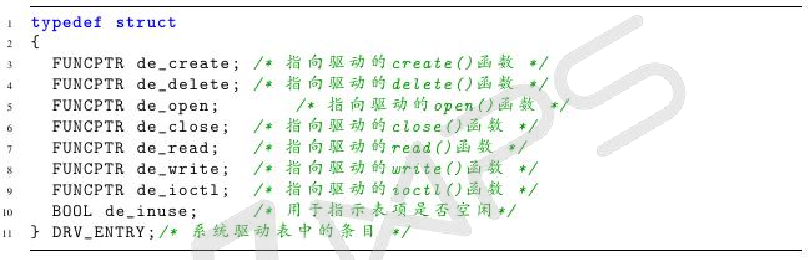
\includegraphics[width=1.0\textwidth]{./graphics/DEVENTRY.pdf}
\caption{DEV\_ ENTRY结构体}\label{fig:DEVENTRY}
\end{figure}

	DEV\_ ENTRY结构体当中的大多数成员都是函数指针,他们用于指向所注册的驱动程序中的一个用于完成特定功能的实际函数,这些函数的功能要符合IO系统预定义好的规则,这些函数被加入到系统驱动表中之后就可以完成与用户层提供的标准函数接口对接\cite{VxWorks内核解读}\cite{VxWorksDriverAPI}\cite{Wind2003VxWorks}。在DEV\_ ENTRY结构体当中唯一不是函数指针的成员是一个布尔类型的 de\_ inuse 成员,若该成员为FALSE则表示该表项目前是未被使用的状态,即该表项没有被任何的驱动所注册。

	VxWorks当中给我们提供了一个驱动的注册函数iosDrvInstall(),使用该函数注册我们的驱动之后,系统驱动表就会分配一个未被使用的表项给该驱动,然后使用iosDrvInstall()所提供的的参数来填充系统驱动表当中的指针,并将de\_ inuse置为TRUE的状态,一个驱动程序不需要实现所有的IO函数,对于实现的函数,在注册时直接将其指针置为NULL即可。

\noindent \textbf{3. 系统描述符表}

	系统描述符表用于管理当前系统中所打开的所有文件描述符,VxWorks中系统描述符表的底层实现也是一个数组。每次执行open()调用成功之后,系统就需要从系统描述符表中分配一个表项给程序使用,并将文件描述符的表项索引作为文件描述符的ID返回给应用程序。之后应用程序直接通过这个ID就可以对文件进行操控,无需每次都是用文件名。
	在VxWorks中,标准输入、标准输出、标准错误输出虽然使用 0,1,2 三个文件描述符来表示,但是它在底层的实现上可能并不是占用了三个文件描述符表的表项,而是只占用一个表项,即三个文件描述符指向同一个文件描述符的表项\cite{VxWorks内核解读}\cite{An2003Implementation},这一点是需要注意的。
		
	
系统文件描述符表中每一个表项都使用 FD\_ ENTRY 这个结构体来表示,这个结构定义在内核的头文件iosLibP.h 中,其定义如\autoref{fig:FDENTRY}所示。


\begin{figure}[!h]
\centering
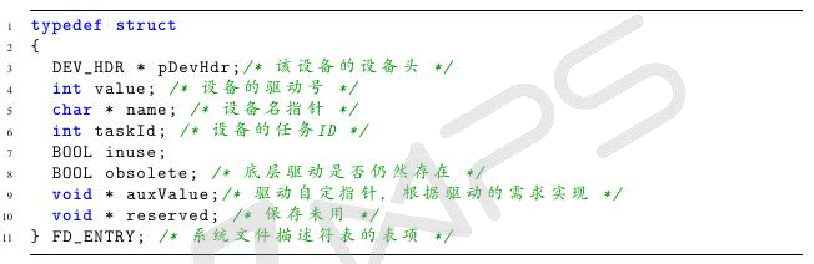
\includegraphics[width=1.0\textwidth]{./graphics/FDENTRY.pdf}
\caption{FD\_ ENTRY结构体}\label{fig:FDENTRY}
\end{figure}

用户的应用程序每次使用open()系统调用系统文件描述符表中就会增加一个有效表项,该表项的FD\_ ENTRY结构体会根据open()调用的内容来进行填充,每一个文件能够进行的open()调用是有限制的,因为数组的容量是固定的,每个驱动的FD\_ ENTRY结构数组满了之后就无法再对这个设备进行open()操作,此时 open()函数将会失败返回\cite{VxWorks内核解读}。系统会在表中的索引偏移 3 (0、1、2被系统占用)之后找一个最先找到的未使用的id作为文件描述符返回给用户。




	
\subsection{VxWorks 中的信号量机制}
	
	任务间的通信机制用于协调多个任务之间的活动,VxWorks内核当中为我们提供了丰富的任务间通信机制,包括共享内存、信号量、消息队列、管道、信号、Sockets等\cite{胡明民2012基于实时操作系统}\cite{冯云贺2014基于}。在我们调试通道的信息传输中需要设计一个特殊需求的USB转串口驱动,在驱动当中需要使用信号量机制
	来确保对驱动内部缓冲区中的数据正确、有序的读写,因此我们有必要先了解一下VxWorks下的信号量机制。

	
	信号量是一种在程序的设计当中最常使用的通信机制,其主要作用是线程间的同步和互斥。VxWorks中提供POSIX信号量的同时还设计了专门的wind信号量,POSIX信号量的使用主要是为了方便程序的移植。
	和POSIX信号量的不同之处在于,VxWorks中设计的wind信号量为VxWorks系统进行了高度的优化,使得其更适用于实时操作系统,能够更快的实现任务间通信。VxWorks中信号量是一个指向SEMAPHORE类型的结构指针,提供了二进制信号量、互斥信号量、计数信号量三种类型的信号量机制,他们适用于解决不同类型的问题。
	
\begin{itemize}
\item 二进制信号量\\
	二进制信号量是最快、最通用的信号量,既可以用于同步也可以用于资源计数。wind的二进制信号量所需系统开销最少,适用于高性能的需求。二进制信号量在资源可用时标记为FULL,在资源不可用时标记为EMPTY。在VxWorks中二进制信号量使用函数semBCreate()来创建,二进制信号量的提取和释放过程如\autoref{fig:erjinzhiTiQu}和\autoref{fig:erjinzhiShiFang}所示。

\begin{figure}[!h]
\centering
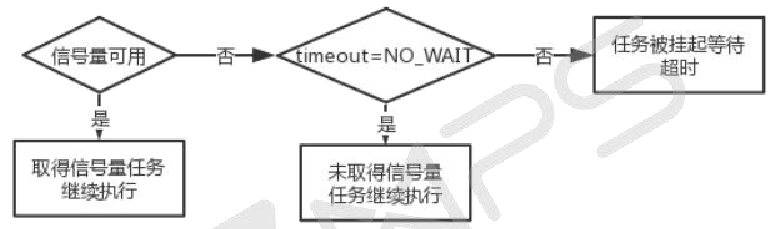
\includegraphics[width=13cm , height=10cm]{./graphics/erjinzhiTiQu.pdf}
  \caption{提取信号量}\label{fig:erjinzhiTiQu}
\end{figure}

\begin{figure}[!h]
\centering
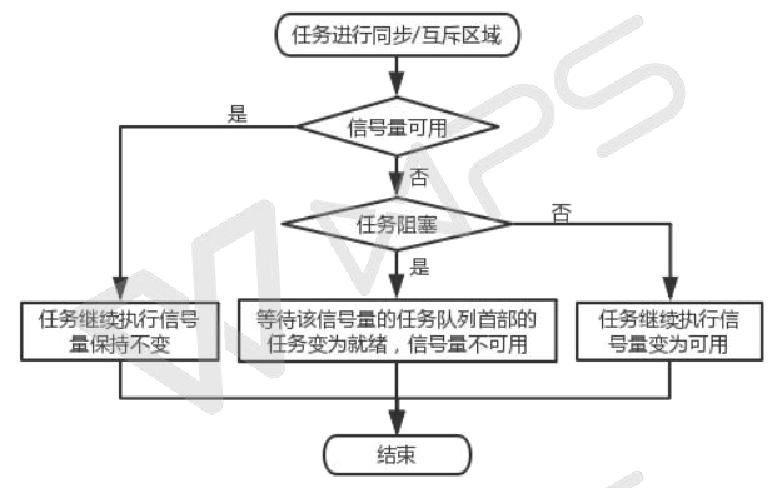
\includegraphics[width=13cm , height=10cm]{./graphics/erjinzhiShiFang.pdf}
  \caption{释放信号量}\label{fig:erjinzhiShiFang}
\end{figure}


\item 互斥信号量\\
	互斥信号量可以看做是一种特殊的二进制信号量(资源数为1),它优化了互斥、优先级继承、删除安全等问题,这使得它能够更好的服务于任务间的互斥需求;互斥信号量的基本行为和二进制信号量是一致的,但是互斥信号量只能够用于互斥,不能够用于同步,该信号量只能够由获得的该信号量的进程来进行释放,不能够由其它的进程进行释放。它使用SEM\_ INVERSION\_ SAFE和SEM\_ Q\_ PRIORITY选项来使得该信号量能继承优先级算法,以此解决优先级的倒置问题;使用SEM\_ DELETE\_ SAFE选项来解决删除安全问题,在VxWorks中互斥信号量使用系统提供的semMCreate()函数来创建;
	
\item 资源计数信号量\\
	资源计数信号量也是一种特殊的二进制信号量(资源数较多),它会跟踪信号量增加、删除的次数,每次释放一个信号量,内部的计数器就会执行加一操作,每次提取一个信号量,内部的计数器就会执行减一操作,当计数器为0时,表示没有可供使用的资源,此时提取信号量的操作就会被阻塞,在VxWorks中资源计数信号量使用系统提供的semCCreate()函数来创建。

\end{itemize}
	
三种信号量的释放操作都是使用semGive()函数;提取操作都是使用semTake()函数,在提取信号量是我们可以选择是否允许超时,超时可以作为解决阻塞的一种方法。



\subsection{USB技术}
	USB(Universial Serial Bus)作为PC领域的最新型的接口技术,目前已被各个PC厂家所支持,并且在各类外设当中都广泛的采用USB接口。USB的开发技术也已经很成熟,通用串行总线开发者论坛(USB Implementers Forum,USB IF)目前制定了三种USB接口标准:USB1.1,USB2.0和USB3.0。USB采用菊花链的形式连接所有的设备,最多可以连接127个设备,USB的总线拓扑结构如\autoref{fig:USB体系结构}所示
\begin{figure}[!h]
\centering
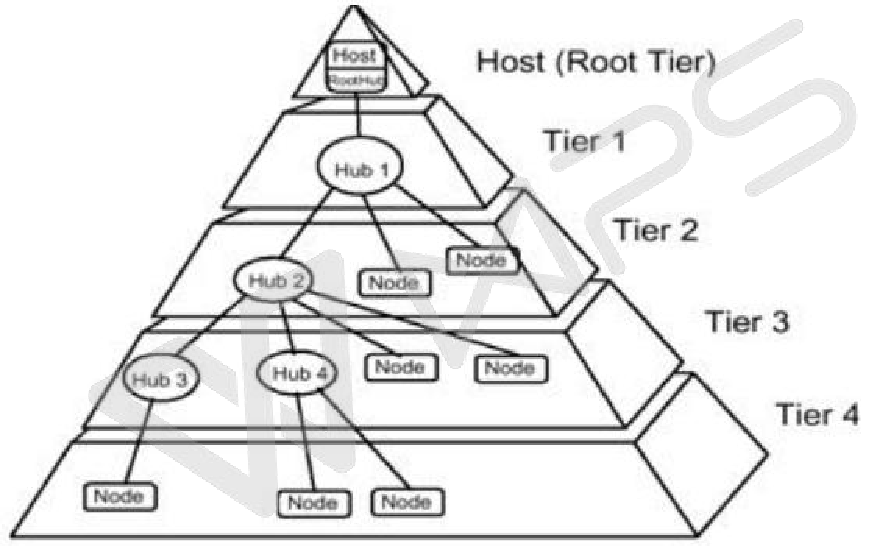
\includegraphics[width=1.0\textwidth]{./graphics/usb-structure.pdf}
\caption{USB总线拓扑结构}\label{fig:USB体系结构}
\end{figure}


USB的体系结构由三个部分组成,分别是USB主机(Host)、USB集线器(Hub)、USB设备(Device)。其中我们需要了解的关键部分是USB主机和USB设备。

\\
	
\noindent \textbf{1. USB主机}
	
	USB主机是USB体系中的核心,且系统中只允许一个USB主机存在。USB主机上的USB接口是USB主控制器,其控制着总线上所有USB设备数据通信。对于USB的体系结构而言,其数据的传输都是USB主机端发起的,非主机端(设备端)只能够被动的进行响应。USB主机需要完成的功能包括检测设备的热插拔、管理主机和设备之间的信息(控制和数据)流\cite{李雪红2004USB}\cite{莫宏伟2001USB}。


\\

\noindent \textbf{2. USB设备}

	USB设备指的是提供具体功能的而外部USB设备,是相对USB主机而言的,它们受USB主机的控制,只能对主机的请求进行被动响应。USB主机端会在检测到USB设备的动作之后会通过默认管道和USB设备进行通信,对其进行必要的初始化配置,并给设备提供适合的驱动程序(如果有的话),一个USB设备会通常会有很多的属性,它会通过这些属性来完成主机的配置要求。一些USB设备的属性如下:
	\begin{itemize}
	\item \textbf{描述符(Descriptor)属性}\\
	描述符是USB协议中定义的一套用来描述USB设备的功能和属性的固定结构,我们可以通过描述符了解设备的各种属性,描述符又分为设备描述符、配置描述符、接口描述符、端点描述符、字符串描述符\cite{张杰2008基于}\cite{边海龙2004USB}除此之外,设备还可以提供自己专用的描述符,分为设备类描述符和供应商自定义描述符,我们使用的USB口转串口设备就不属于一个标准的USB设备,它会为我们提供供应商自定义的描述符,我们使用需要使用它来对设备进行识别。
	
	\item \textbf{类(Class)属性}\\
	由于USB协议支持许多的外围设备,而这些设备又可以根据功能来分成一些相近的类,如打印机类、键盘类等。这样主机端就可以为这些功能相近的设备提供一个类驱动,类驱动可以用于驱动所有属于同一类的设备,不需要再为每一个设备提供一个完整的驱动程序。这大大的方便的设备的制造商,他们的设备只需要符合某一类的驱动,就可以使用该类驱动程序来驱动其设备,之后只需要实现简单的包含有设备特性的客户端驱动即可,若设备没有特殊的特性,则直接使用类驱动即可\cite{李雪红2004USB}。	
	
	\item \textbf{功能(Function)/接口(Interface)属性}\\
	功能或接口是USB协议中定义的设备的某种能力,Function是从功能角度来说的,从设备的角度来说,被称为Interface。对于一个设备他可以拥有很多个不同的接口,每一个接口负责完成设备的一个特定的功能,并且这个接口具体实现什么样的功能并不是固定的,当USB设备处于可配置状态的时候能够通过控制命令来改变某一个接口的功能,一个接口能够具有什么样的功能会在USB的接口描述符中进行描述。
	
	\item \textbf{端点(Endpoint)属性}\\
	端点是USB设备与USB主机逻辑上的通信流的终点,每个设备都拥有一个可独立进行操作的端点集合,且每个端点在使用时都要先初始化其数据传输方向(IN/OUT),即使端点号相同但是传输方向不同的通信点也是不同的端点\cite{李雪红2004USB}。
	
	\item \textbf{管道}\\
	管道可以看做是设备上的一个端点和主机上的软件的联合体,设备和主机间的数据传输要基于管道进行。在USB的通信过程中首先要建立一个管道才能够进行数据的传输,USB设备在和主机通信时都会建立一个默认的管道,这个管道对应的端点是默认端点0,之后需要自己使用其它的端点来建立我们的数据传输过程中需要使用的输入或输出管道。在我们的USB口转串口驱动中会为每一个设备建立两个管道,一个批量输出管道和一个批量输入管道。
	
	\item \textbf{设备地址}\\
	设备地址用于区分USB系统中的一个USB设备的特殊标识,设备地址会在设备初始化之后由主机进行分配且是唯一的。设备地址单元共有7bit,其中地址0是缺省地址,在设备初始化的时候使用,理论上系统可以区分127个USB设备\cite{李雪红2004USB}。
	\end{itemize}	



\noindent USB规范规定了USB主从设备之间的四种传输方式,每种方式有各自的用途\cite{USB总线接口开发指南}:

\begin{itemize}
\item \hei{控制传输}:控制传输USB传输方式中最重要、最复杂的一种,它适用于少量、对时间和速率无要求的场合,一个USB设备插入主机之后就是使用这种传输方式来读取设备的地址和描述符等信息。所有的设备都会在其0号端点的缺省管道当中支持控制传输\cite{张杰2008基于}。
\item \hei{批量传输}:批量传输有两种最基本的事物类型:BULK\_ IN和BULK\_ OUT,其主要用于处理对数据传输速率不是很高的情况,批量传输使我们的USB口转串口设备所使用的主要传输传输方式,每次有数据需要传输时我们都会构建一个IRP使用批量传输将其传出或传入。
\item \hei{中断传输}:中断传输也有两种基本的事务:IN和OUT,其主要是为那些要快速实现主机和设备的交互,但是数据量很小、对服务时间有要求的情况而准备的。
\item \hei{等时传输}:等时传输也是由基本的IN和OUT两种事务组成,主要用于处理大量、恒速、对时间周期有要求的数据。等时传输只有全速和高速设备才支持,低速设备不支持\cite{张杰2008基于}。
\end{itemize}


	

\section{本章小结}
	本章重点介绍了本次的VxWorks调试通道的整体架构,并介绍了介绍了各个部分的设计方案,最后介绍了在本次的设计当中所需要使用关键技术和所需了解的重要知识,主要包括VxWorks下的驱动开发必须的结构、驱动中所需使用的VxWorks的通信机制、缓冲区技术、USB技术。下面将要讨论VxWorks下的调试通道的详细的设计细节和具体的实际机制。



























\clearpage
\chapter{驱动程序的设计和实现}
	
	设备驱动程序在操作系统中框架是操作系统的设计人员在设计操作系统时已经制定好的,	所以在进行驱动程序的开发时需要开发人员对操作系统和设备的硬件体系具有相当的了解,而且驱动程序的性能、可靠性也制约着系统的性能和可靠性。	


\section{VxWorks上的USB开发}\label{sec:USB开发}
	在VxWorks当中I/O框架的实现放在内核文件ioLib.c当中,我们将它称为上层接口子系统,因为它负责给上层应用提供I/O接口,但是该接口并不会完成具体请求的实现,他只会在进行简单的处理之后将请求转发给I/O子系统,具体请求的处理工作会被发送到I/O子系统当中来处理。I/O子系统的定义放在在内核文件iosLib.c当中,I/O子系统对用户层而言通常是透明的,用户层一般不会直接调用I/O子系统中的函数,它是作为上层接口子系统与下层驱动系统的中间层来使用的。VxWorks的当中内核驱动层次结构如\autoref{fig:VxWorks内核驱动层次结构}所示。	

\begin{figure}[!h]
\centering
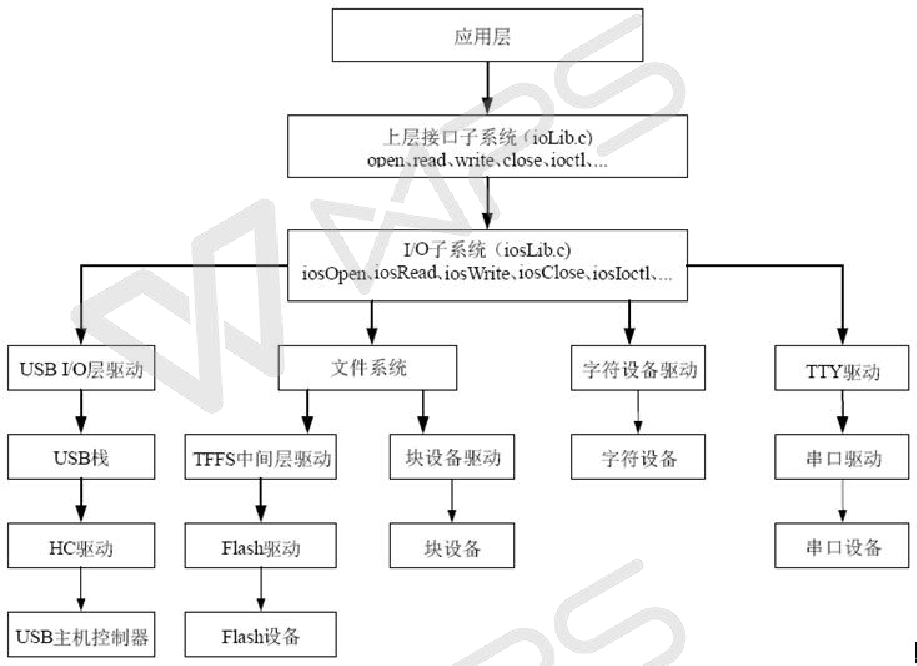
\includegraphics[width=0.9\textwidth]{./graphics/vxworks-kernel-diagram.pdf}
\caption{VxWorks驱动内核层次结构}\label{fig:VxWorks内核驱动层次结构}
\end{figure}	
			
	从\autoref{fig:VxWorks内核驱动层次结构}当中我们可以看出主机端USB驱动在VxWorks当中的层次结构,但是VxWorks作为一个嵌入式系统,其作为USB的主/从端的可能性都是存在的,所以其上也有USB从端驱动栈的实现。但我们本次需要使用的是其主机栈,在VxWorks当中USB驱动程序堆栈的开发符合的是通用串行总线规范2.0标准,VxWorks中的USB主机端内核驱动层次如\autoref{fig:VxWorks_USB_kernel_diagram}所示。VxWorks中的将USB协议在主机端分成三层来实现,分别是客户端驱动程序(Client Driver)、USB驱动(USBD)、主机控制器驱动(HCD),每一层完成不同的功能。其通信的逻辑结构和PC端的软硬件结构如\autoref{fig:USB通信结构}所示。

\begin{figure}[!h]
\centering
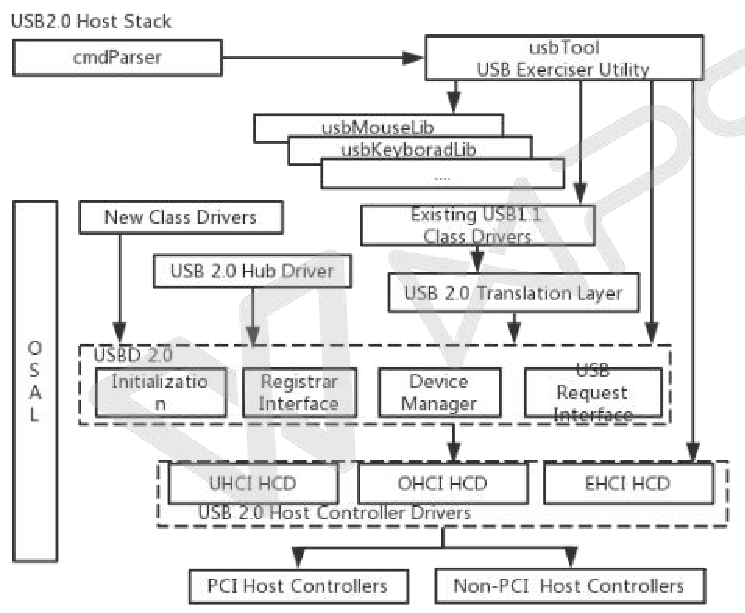
\includegraphics[width=0.9\textwidth]{./graphics/VxWorks_USB_kernel_diagram.pdf}
\caption{VxWorks下USB内核驱动层次结构}\label{fig:VxWorks_USB_kernel_diagram}
\end{figure}

\begin{figure}[h]
\centering
  \begin{subfigure}[b]{0.4\textwidth}
  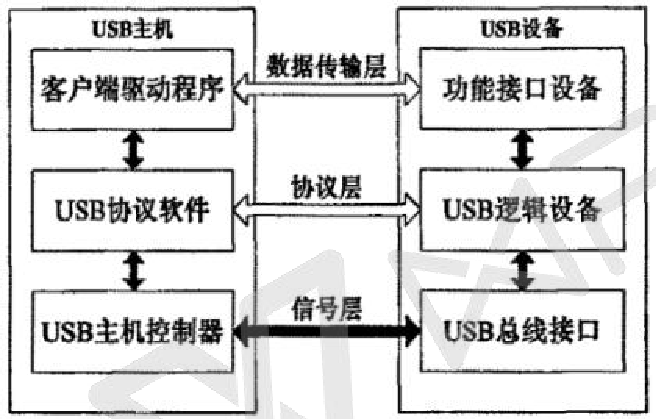
\includegraphics[width=1.0\textwidth]{./graphics/USB-device-structure-diagram.pdf}
  \caption{USB通信的逻辑结构}\label{fig:usb通信逻辑结构}
  \end{subfigure}
  ~
  \begin{subfigure}[b]{0.5\textwidth}
  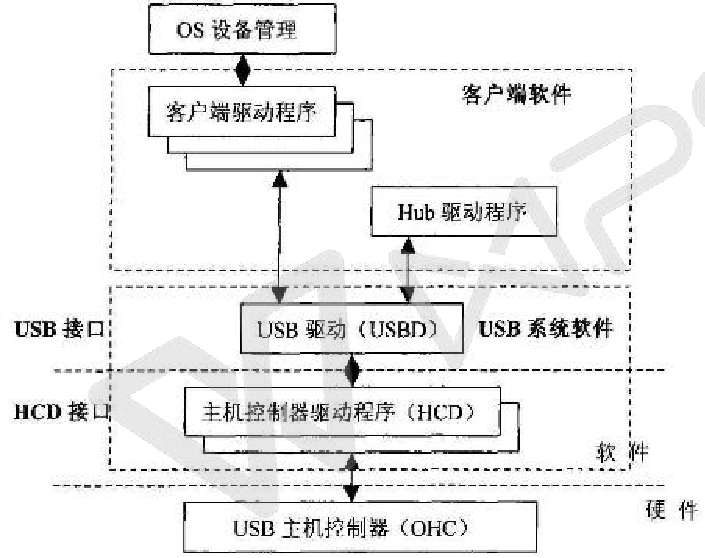
\includegraphics[width=1.0\textwidth]{./graphics/USB-PC-structure.pdf}
  \caption{USB主机端软硬件结构}\label{fig:usb-PC}
  \end{subfigure}
\caption{USB通信结构}\label{fig:USB通信结构}
\end{figure}

	
	客户端驱动程序的功能是完成对不同类型设备的功能驱动。本次设计中所要完成的USB口转串口的驱动要完成的就是客户端驱动。USB口转串口驱动会构建USB I/O请求包(I/O request,IRP)来向USBD层发出数据接收或者发送的请求,IRP是USB协议中定义的一个抽象概念,我们需要根据所发送的内容和发送的方式来具体的实现一个IRP\cite{李雪红2004USB}。
	
	USBD是USB的核心驱动,其提供了操作系统组件(主要是设备驱动)能够用来访问USB设备的方法,其实现是由操作系统决定的。USBD提供包括USB总线的枚举、总线带宽的分配、传输控制等操作,它还会处理客户端驱动程序发送来的IRP包,并在对IRP请求包进行解析之后将实际的请求映射到适当的HCD或者直接交给主机控制器处理。除此之外USBD负责的内容还包括新设备的动态插拔、电源管理和对客户端驱动程序的维护等。
	
	HCD层提供一个软件抽象来完成USB主控制器的各种事物处理,用于隐藏主控制器的硬件实现细节,HCD只服务于我们的USBD层,对上层应用而言其通常是不能直接访问的。
	VxWorks中HCD层只需要向USBD层注册一个接口函数,所有的USBD层的请求都是用这个接口函数来完成,对于UHCI主机控制器驱动而言他被命名为usbdHcdUhciExec,对于OCHI主控器驱动而言被命名为usbdHcdOhciExec。
	HCD层会将USBD层传输下来的事务调度给主机控制器进行处理,当事物处理完成之后HCD层会将处理结果返回给USBD层。此外它还会完成对主机控制器和根集线器的配置和驱动等操作\cite{李雪红2004USB}。VxWorks中本身已经集成好了对几种常用的主机控制器驱动的支持,包括UHCI主控器、OHCI主控器、EHCI主控器,VxWorks中暂时没有实现xHCI主控驱动。
	
	对于我们的USB口转串口驱而言,我们不再需要实现对物理设备的数据结构抽象,因为VxWorks中的USB HCD层已经为我们实现好了物理层的抽象,同时还给我们提供了USBD层,因此我们只需要实现USB主机三层结构当中的客户端驱动程序即可,使其能够驱动特定的USB设备正常工作。在客户端驱动当中,我们需要完成IO系统的各类接口的实现、完成驱动需要实现的特殊功能的实现、将驱动集成到系统中等工作。
	


\section{CP2102开发}
	除了驱动程序之外,USB口转串口的实现还需要硬件来作为支撑,PC机上本身并没有USB/RS-232的转换器,
	对于USB/RS-232转换器的设计通常有两类实现方式:一类是使用包含有USB单元的微处理器从底层的硬件和固件进行全面系统的设计,这样的控制器有PCI16C745、68HC705JB4和C541U系列等\cite{USB与RS232接口转换器的设计},但是使用这种方式从头开始设计存在难度大,系统复杂等问题,不符合我们本次设计工作的需求。
	第二类方法是采用市场上设计好的USB/RS-232双向转换芯片,这类芯片有CH341,CP2102、FT232BM等,我们在此处的设计即使用了CP2102芯片作为USB/RS-232转换器,这样设计的好处是不需要编写转换器芯片的固件,节约开发时间,由于这个技术已经很成熟,大多的USB口转串口的解决方案都会采用这种已经设计好的集成芯片来作为转换器。
	
	CP2102是SILICON LABORATORIES推出的USB与RS232接口转换芯片,
	它包含有一个USB2.0全速功能控制器,EEPROM,USB收发器,振荡器和异步串行数据总线(UART),在SILICON给出的文档当中已经帮我们给出了一个最简单 CP2102的使用方式的电路框图,如\autoref{fig:cp2102电路框图}所示。
\begin{figure}[!h]
\centering
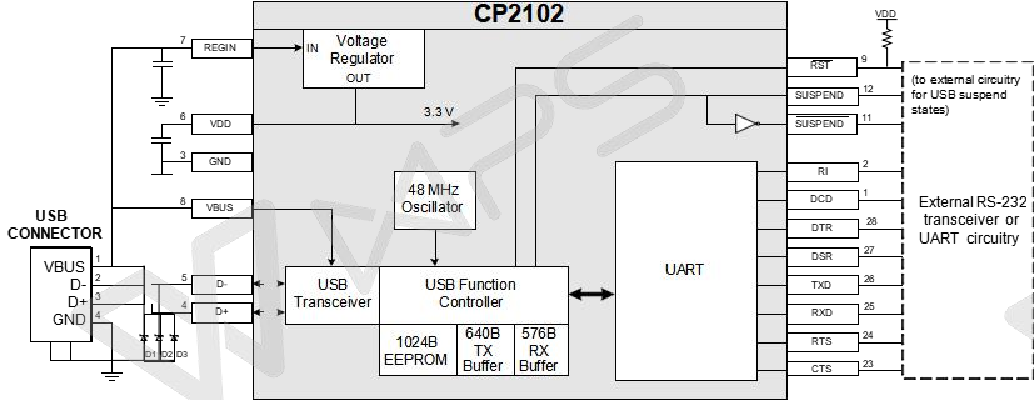
\includegraphics[width=1.0\textwidth]{./graphics/cp2102-circuit-diagram.pdf}
\caption{cp2102电路框图}\label{fig:cp2102电路框图}
\end{figure}

\begin{enumerate}
\item CP2102的USB功能控制器和收发器:CP2102的内置的USB功能控制器符合USB2.0协议,它负责管理USB和UART之间的所有数据和控制传输。
\item 异步串行数据总线(UART)接口:CP2102的UART接口支持接收、发送、控制、握手信号,而且支持对UART数据格式和波特率进行编程控制。可以使用的数据格式和波特率见\autoref{fig:CP2102可配置参数}。
\item 内部EEPROM:CP2102内部集成了一个1K的BEEPROM,在其中存储了一些设备的特定信息,包括厂商ID、产品ID、产品说明、电源参数、器件版本号和器件序列号等\cite{CP2102}。如果OEM没有为设备的EEPROM写入数据的话,那么设备会自动的使用一组默认的数据,如\autoref{CP2102DefaultConfigure}所示。
\end{enumerate}

\begin{figure}[!h]
\centering
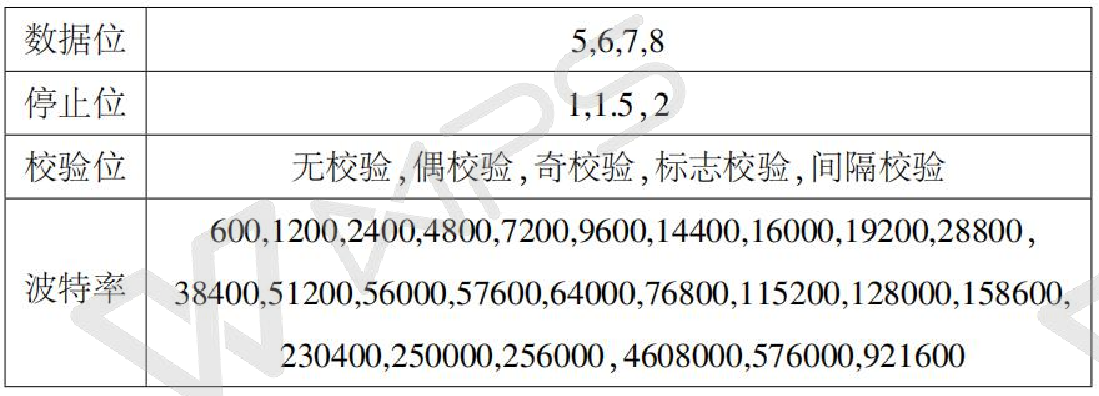
\includegraphics[width=1.0\textwidth]{./graphics/CP2102ChioceConf.pdf}
\caption{cp2102可选配置参数}\label{fig:CP2102可配置参数}
\end{figure}

\begin{figure}[!h]
\centering
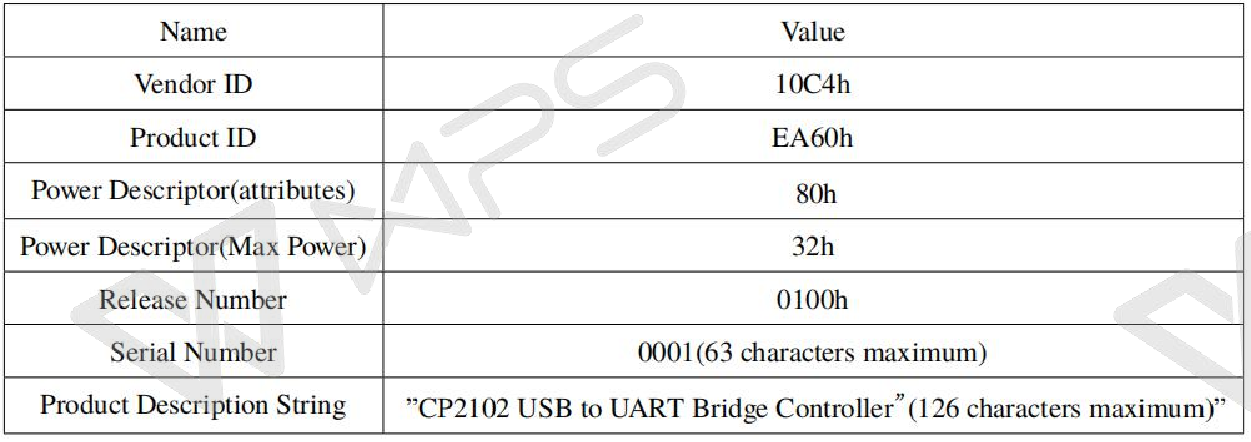
\includegraphics[width=1.0\textwidth]{./graphics/CP2102DefConf.pdf}
\caption{CP2102默认配置表}\label{CP2102DefaultConfigure}
\end{figure}
	使用CP2102进行串口扩展的时候只需少量外部器件,
	CP2102当中的协议控制单元会对来自USB接口的命令进行解析,然后对UART接口进行配置。UART的部分可配置参数如\autoref{fig:CP2102可配置参数}所示,
	CP2102当中的拥有一个576B的接收缓冲区和一个640B发送缓冲区,这些缓冲区可以部分的解决USB和RS-232之间的速率不匹配的问题。以从计算机到外设的数据传输为例。当USB转串口设备连接到PC的USB总线上后,PC会对其进行初始化并在识别出该设备后启动支持该设备的客户端驱动;计算机上的驱动程序会将数据包传输给USB接口(通常使用批量传输的方式),设备从USB接口提取出数据并保存在数据缓冲区中,UART接口再从数据缓冲区中将数据取走并发送出去,从外设传输数据到计算机的方式则相反\cite{李雪红2004USB}。	
	
	在我们本次的设计当中我们并不会去完成CP2102的外部电路的设计工作,而是选择市场上已经封装好的模块。我们本次使用的设备如\autoref{fig:cp2102模块正反面}所示。我们所需要做的是了解CP2102的原理和功能,能够对其进行正确的开发工作。
\begin{figure}[h]
\centering
  \begin{subfigure}[b]{0.4\textwidth}
  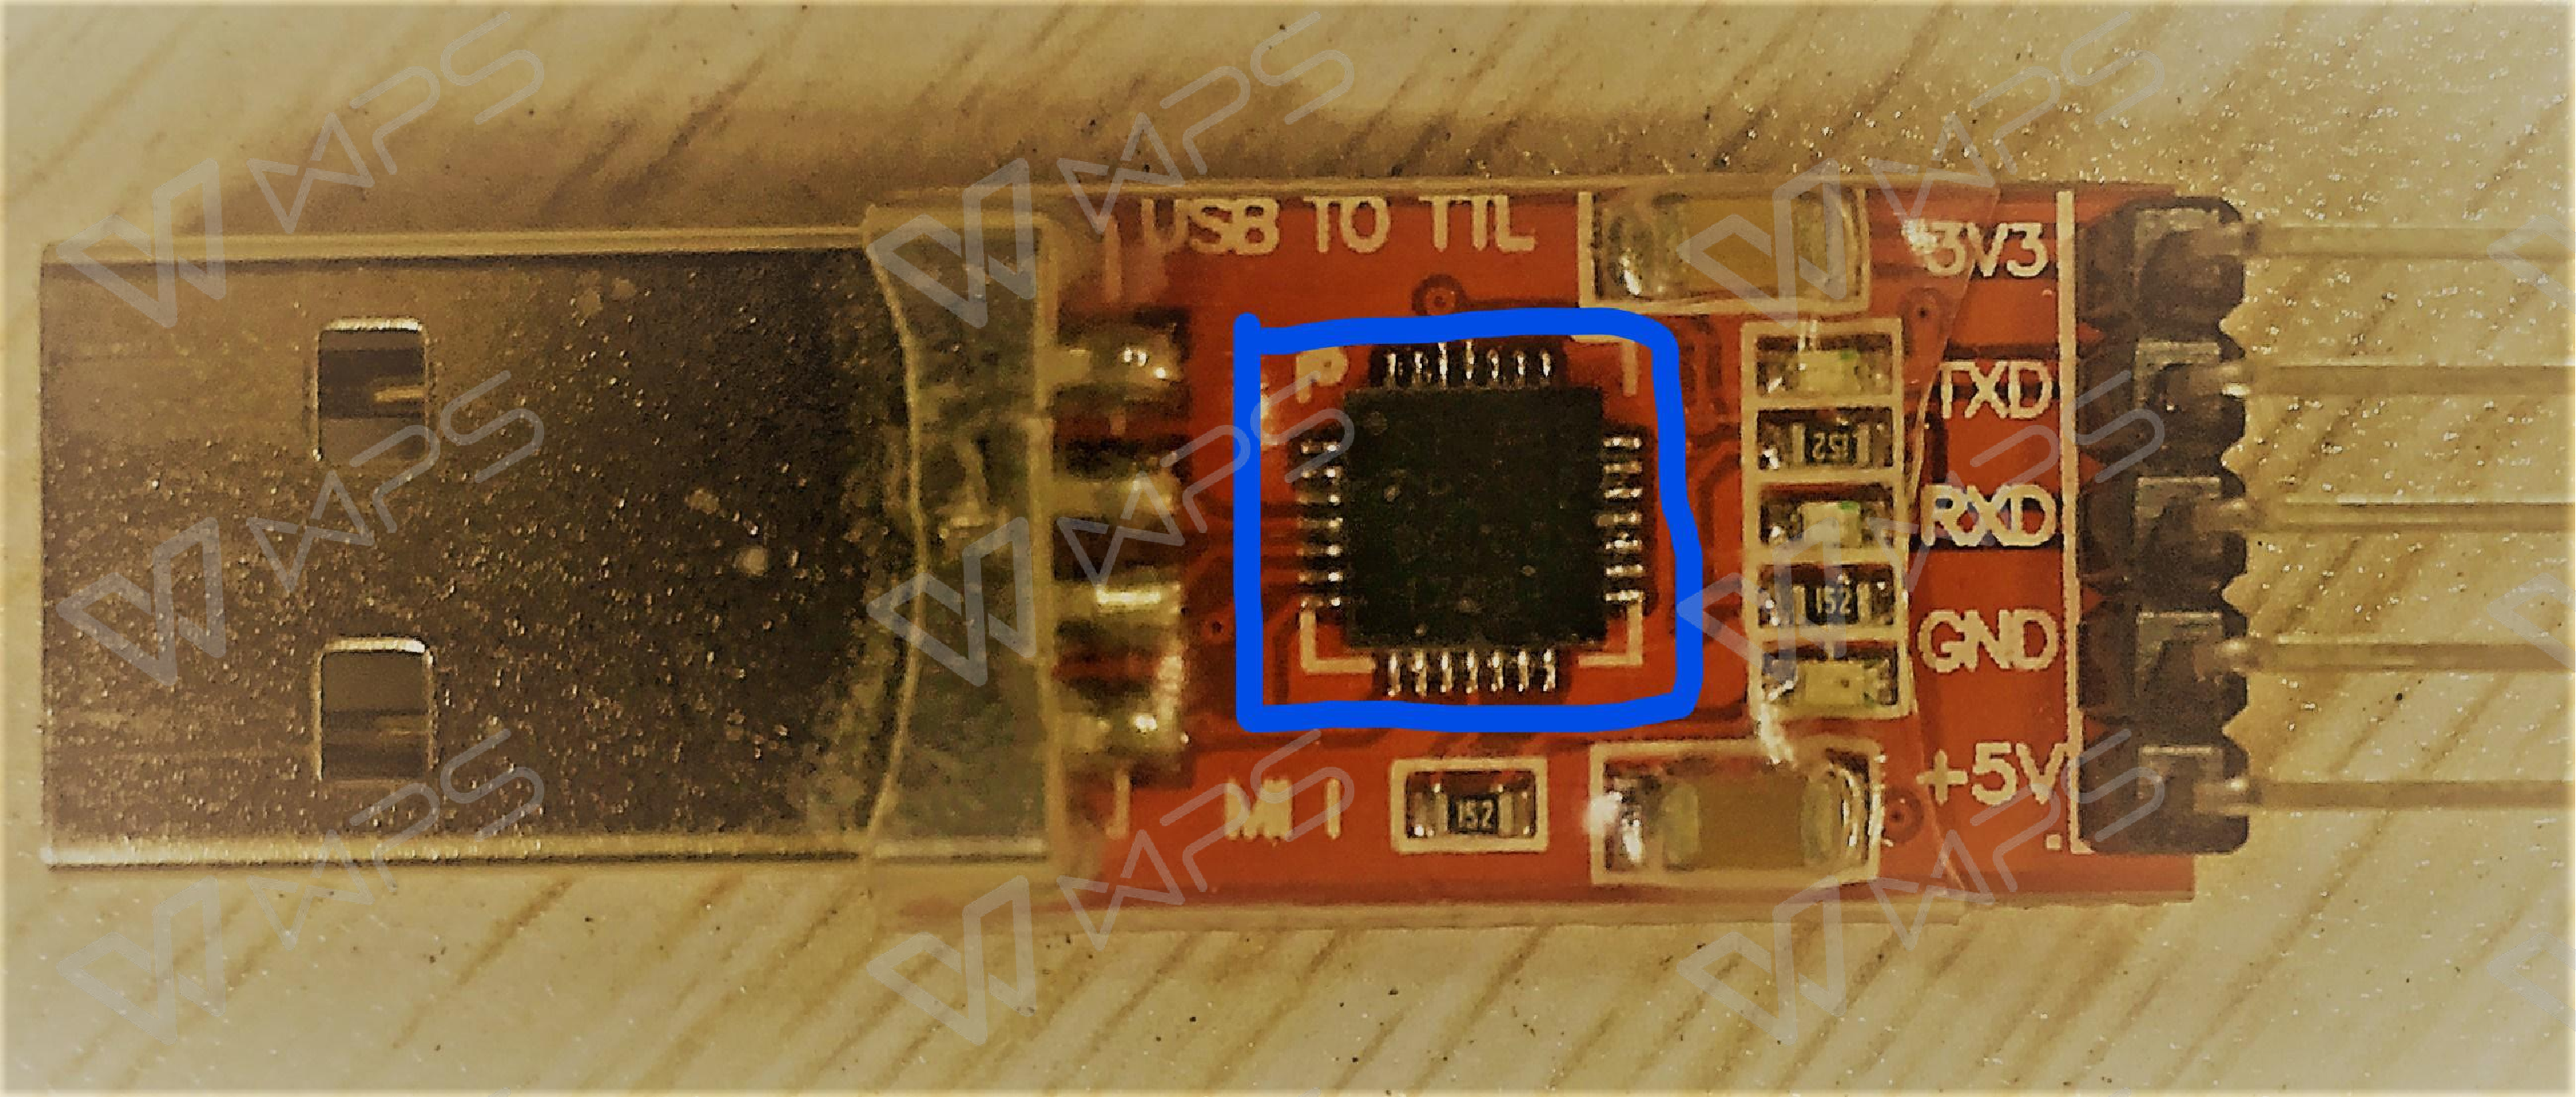
\includegraphics[width=\textwidth]{./graphics/cp2102Front.pdf}
  \caption{CP2102模块正面}\label{fig:cp2102Front}
  \end{subfigure}
  ~
  \begin{subfigure}[b]{0.4\textwidth}
  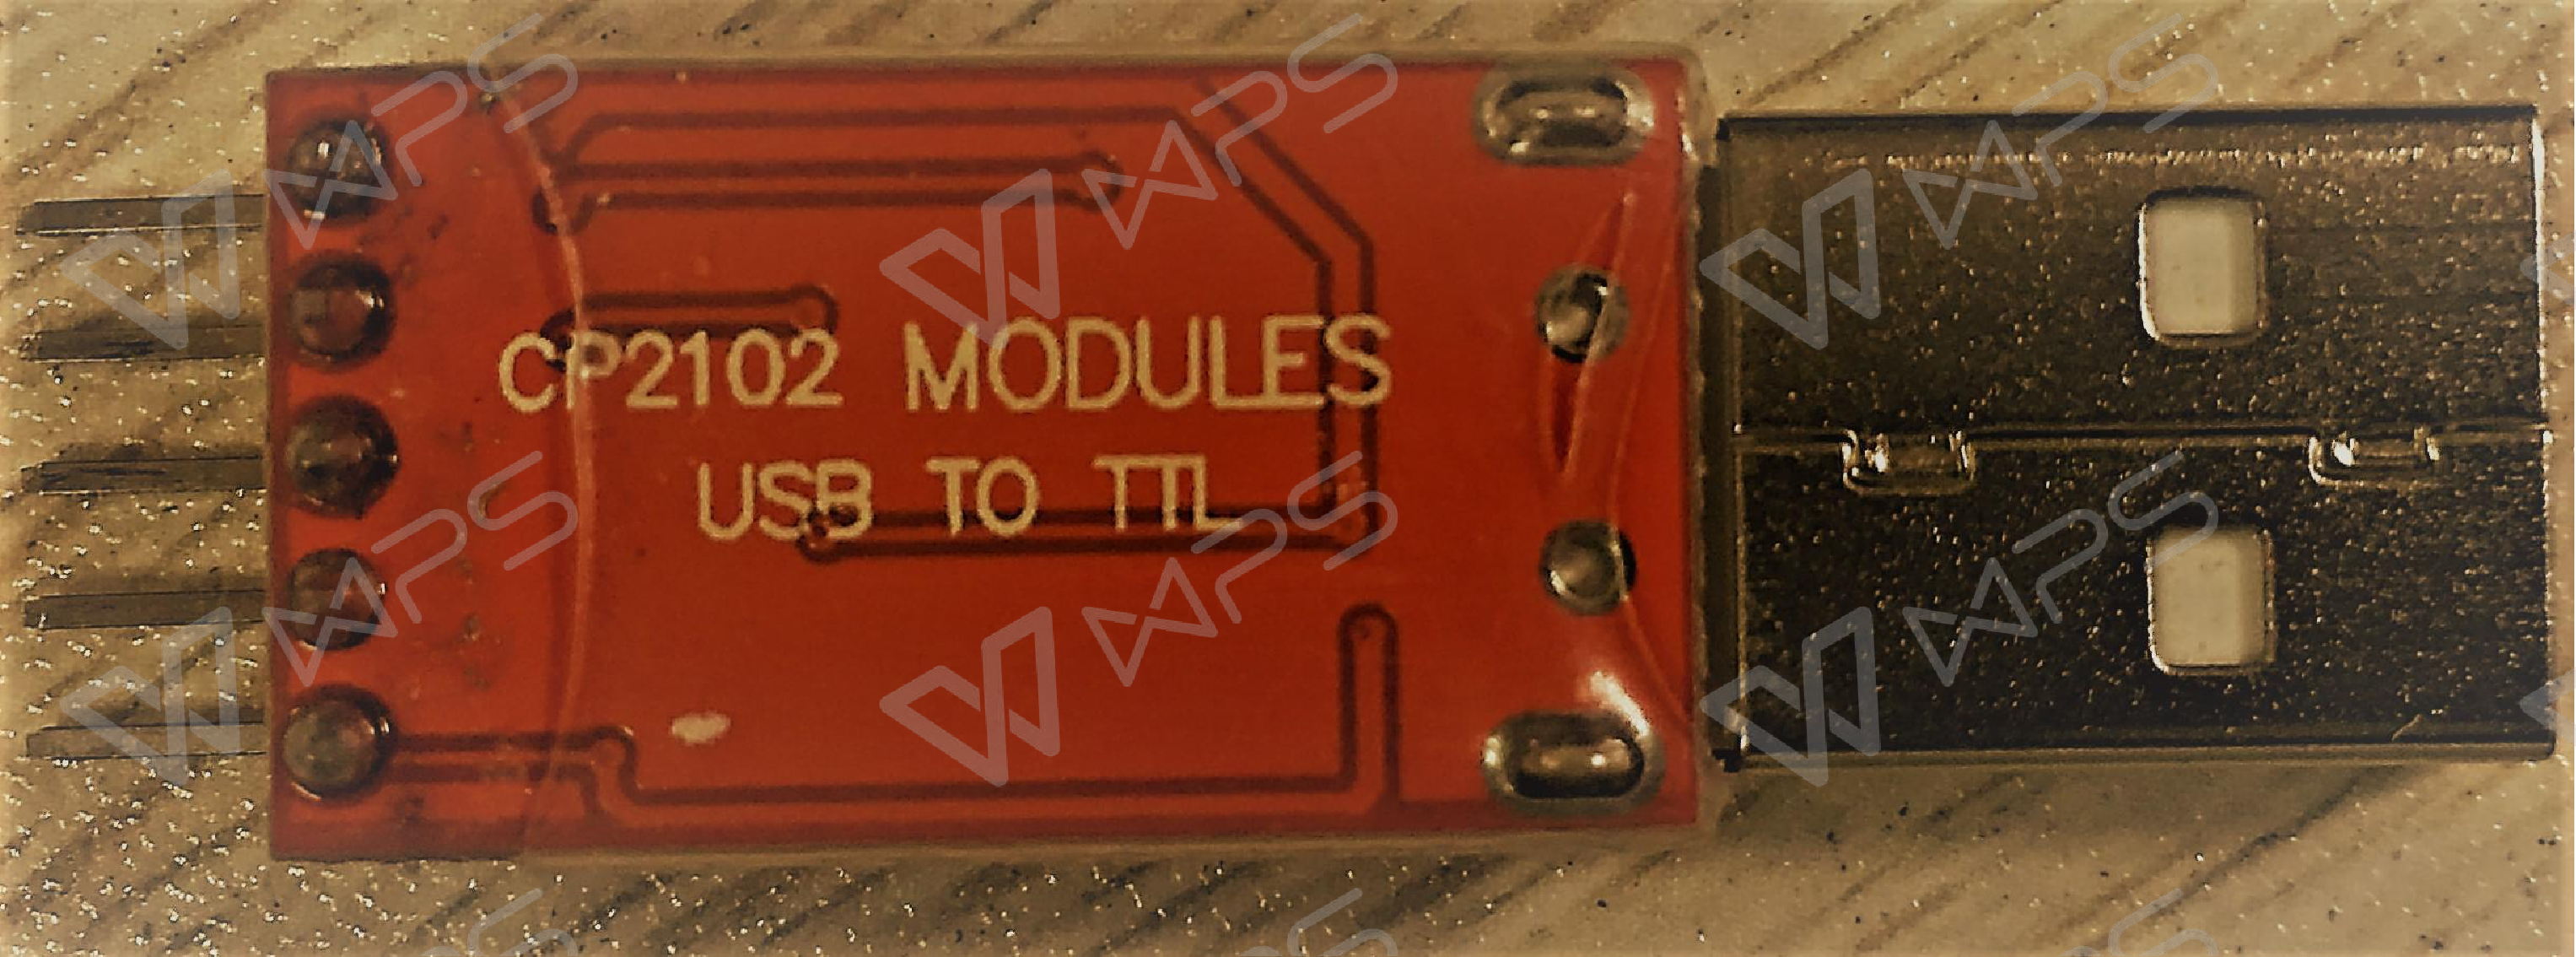
\includegraphics[width=\textwidth]{./graphics/cp2102Rear.pdf}
  \caption{CP2102模块反面}\label{fig:cp2102Rear}
  \end{subfigure}
\caption{CP2102模块正反面}\label{fig:cp2102模块正反面}
\end{figure}
	

\section{特定需求单设备驱动的实现}

	
	在VxWorks I/ O 当中通常应该经过以下的三个基本步骤来实现一个设备驱动:
\begin{enumerate}
\item 实现对实际物理设备的数据结构抽象(即设备的自定义数据结构);
\item 完成 I/ O 系统所需要的各类接口及自身的特殊接口(open、read、write等);
\item 将驱动集成到操作系统中。
\end{enumerate}

	无论驱动程序的开发人员要完成一个什么样的驱动程序,其都有一些系统规定的标准的模块,以方便控制设备。我们此次驱动程序需要实现的框架部分主要包括cp210xDrvInit()、cp210xDevOpen()、cp210xDevClose()、cp210xDevIoctl()、cp210xDevWrite()、cp210xDevRead()、cp210xDrvUnInit()等函数,如\autoref{lab:驱动程序的关键模块}所示 ,在这些模块当中关键要处理的内容是对数据的传输工作和对设备的控制工作,数据的传输要用到缓冲区和用于进行同步和互斥操作的信号量。
\begin{table}[!h]
\centering
\begin{tabular}{|c|c|}
\hline
{模块} & {作用} \\
\hline
{cp210xDrvInit()} & \tabincell{c}{这个模块用来初始化驱动程序,主要是与设备无关的一些\\全局变量并向系统注册该驱动} \\
\hline
{cp210xDevOpen()} & \tabincell{c}{这个模块用来转接I/O子系统分发过来的open()操作,实现设备的打开,\\返回设备的指针} \\
\hline
{cp210xDevClose()} & \tabincell{c}{这个模块用来转接I/O子系统分发过来的close()操作,实现设备的关闭,\\对设备占用资源进行清理} \\
\hline
{cp210xDevIoctl()} & \tabincell{c}{这个模块用来转接I/O子系统分发过来的ioctl()操作,\\实现对设备的一些特定的控制操作} \\
\hline
{cp210xDevWrite()} & \tabincell{c}{这个模块用来转接I/O子系统分发过来的write()操作,\\实现对设备进行数据的写入} \\
\hline
{cp210xDevRead()} & \tabincell{c}{这个模块用来转接I/O子系统分发过来的read()操作,\\用于从设备读取数据。} \\
\hline
{cp210xDrvUnInit()} & \tabincell{c}{这个模块用来卸载驱动程序,将驱动从系统驱动表中删除,\\并清理该驱动程序所占用的全部资源} \\
\hline
\end{tabular} 
\caption{驱动程序的关键模块}\label{lab:驱动程序的关键模块}
\end{table}


	由于对于仅支持单设备驱动程序是基于特定的需求而具体定制的,所以该设备的驱动程序的实现流程与通常的支持多设备的驱动的初始化流程存在差异。具体的需求为:\\
\hei{1. 驱动中支持的设备名是固定的,无论具体的设备是否连接上,都可以往这个设备中写入数据。}\\
\hei{2. 驱动程序中要有缓存一定数据的能力,一旦设备连接之后就能够检查缓冲区中是否有数据,有数据则将其发送出去。}

	由于需要在设备未连接时就能够往设备中写入数据,且设备名为固定的,那么就必须调整驱动的初始化流程,使得其能够支持这一特性,通常驱动都是在设备加载之后再将其加入到系统设备表和系统驱动表当中,那么此时我们就需要先将一个固定的设备名加入到系统设备表当中,并为其初始化好设备的缓冲区,具体的设计如下文所示。



\subsection{设备的自定义结构}
	底层驱动都要为其所驱动的每一个设备维护一个设备的自定义数据结构,这个结构的第一个成员必须是DEV\_ HDR结构体,DEV\_ HDR这个结构是给系统维护该设备的驱动时使用的,其余的成员为该设备所需保存的关键参数,这些参数都是我们的驱动程序在设备运行时需要使用的,系统不会使用这些参数。对于我们的USB口转串口设备而言,我们需要保存的关键参数有:USB配置、读写缓冲区的指针、接口配置、端点地址等等。关键数据结构的定义如下: 
	
\lstset{language=C}
\begin{lstlisting}
typedef struct cp210x_dev
{
  DEV_HDR cp210xDevHdr; 
  
  UINT16 numOpen;
  USBD_NODE_ID nodeId;
  UINT16 configuration;	
  UINT16 interface; 
  UINT16 interfaceAltSetting;
  UINT16 vendorId;
  UINT16 productId;

  BOOL connected;  
  int trans_len;
  USBD_PIPE_HANDLE outPipeHandle; 
  USB_IRP	outIrp; 
  BOOL outIrpInUse; 
  UINT16  outEpAddr;
  UINT8 trans_buf[64];

  USBD_PIPE_HANDLE inPipeHandle;
  USB_IRP inIrp;
  BOOL inIrpInUse;
  UINT8 inBuf[64];
  UINT16 	inEpAddr;
} CP210X_DEV, *pCP210XDEV;
\end{lstlisting}
\noindent 部分成员的含义如下:

\begin{itemize}
\item DEV\_ HDR:这一成员必须是自定义设备结构的第一个成员,VxWorks 的I/O子系统会把所有的设备结构都看作是这个类型的结构,系统只会识别到DEV\_ HDR结构并对其进行管理,在系统设备表、系统文件描述符表当中都需要使用该驱动中的DEV\_ HDR这个成员。
\item numOpen:用来记录设备被打开的次数,每次调用open()函数打开该设备则numOpen加一,调用close()函数关闭设备则减一。
\item nodeId:用来保存该设备在系统中的唯一ID号。
\item configure、interface、interfaceAltsetting:用来保存设备的描述符中的配置、接口、可变接口信息。
\item vendorId、productId:保存该设备的厂商ID和产品ID,用来识别该设备是否适合我们的驱动程序。
\item outPipeHandle、inPipeHandle:设备的输入/输出端点的管道句柄,每次传输数据时都需要使用该句柄来表明数据传到的哪一个端点。
\end{itemize}






\subsection{驱动初始化} 
	
	底层的驱动程序都要提供一个初始化函数给系统来调用,以便进行驱动程序的注册和初始化驱动必须的资源,这些工作通常是在内核启动过程中进行的,你必须将你的驱动加入到内核的启动列表当中,内核在启动的时候就会调用我们的驱动初始化函数。对于此处的USB口转串口驱动我们定义cp210xDrvInit()为初始化函数,其主要完成驱动所需要的资源的申请和全局变量的初始化,包括创建信号量、向系统注册驱动、创建设备、向USBD层注册。驱动初始化函数的主要流程如\autoref{fig:SDevice-Driver-diagram-a}所示。
	
\begin{figure}[!h]
\centering
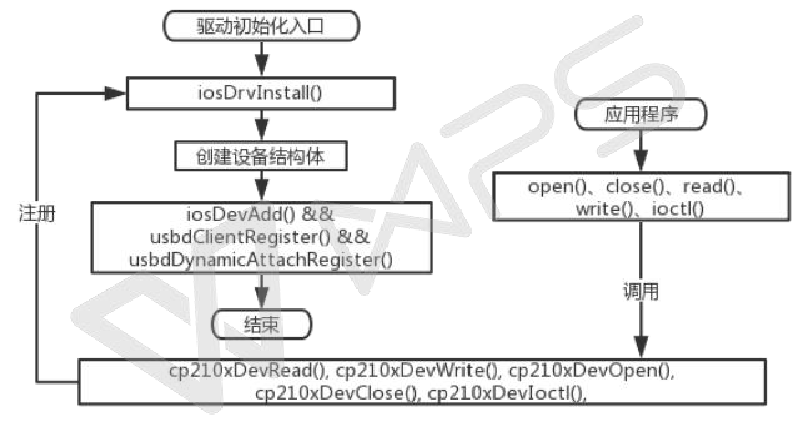
\includegraphics[width=1.0\textwidth]{./graphics/SDev-Drv-Diagram-a.pdf}
\caption{单设备驱动初始化流程}\label{fig:SDevice-Driver-diagram-a}
\end{figure}



	在调用驱动初始化函数时,驱动首先会检查自己是否已经安装过了,若已经安装了则无需再次安装,直接返回即可。我们通常会将驱动的初始化模块放在usrRoot(usrConfig.c)中调用,这样驱动就可以随着内核的启动而启动。但是你也可以将其当做是一个核外的模块来进行启动,在VxWorks中你需要加载驱动程序所在的库,然后直接运行cp210xDrvInit()函数即可。
	驱动初始化时需要初始化我们用来在驱动的运行过程中使用的各种信号量,还需要调用iosDrvInstall()函数安装驱动的I/O函数,将其添加到驱动表当中,在我们的USB口转串口驱动当中不需要实现delete函数和create函数,直接将其指针置为NULL即可。
	
	此处和普通驱动不同的地方是,我们单设备驱动的初始化函数当中就已经初始化好了驱动所需要的缓冲区,并且已经先将设备添加到了I/O子系统当中,此时实际的设备并不存在,添加到系统当中的只是一个“假”设备,只有软件实现,没有实际的硬件支撑,即使此时已经可以打开该设备,向该设备写入数据,但是也只是写入到了系统的缓冲区当中而已,数据并没有发送到任何的硬件上。而普通的驱动程序 中的逻辑应当是在检测到设备插入,并且识别出该设备能够被我们的驱动程序所支持时才给其分配缓冲区、进行设备的初始化工作,最后再调用iosDevAdd()将设备注册到I/O子系统。
	
	在设备成功的添加到I/O子系统之后,系统的设备表当中就会显示该命名为CP210X\_ NAME的设备(CP210X\_ NAME只是一个宏定义,设备名可以自己更改),我们可以在系统中使用iosDevShow命令来进行查看。
	

	在设备注册完之后我们还要将USB客户端驱动还需要向USBD层注册,在\autoref{sec:USB开发}中我们介绍过,USB主机架构将其分为三层来实现,USBD层就是为我们的客户端驱动所服务的,它负责管理USB的中断、热插拔等事件。它给我们提供了注册函数usbdClientRegister()和usbdDynamicAttachRegister(),使用usbdClientRegister()注册之后USBD层才能知道我们的客户端驱动的存在,并将我们的驱动加入到它的服务列表当中,它会给我们的驱动分配一个独一无二的句柄cp210xHandle,以后对USBD层进行操作是只需传递cp210xHandle这个独一无二的句柄USBD层就能区分是哪一个驱动在发送数据。
	
	usbdDynamicAttachRegister()用于注册我们的驱动所感兴趣的设备的热插拔事件,并像USBD层注册一个回调函数cp210xAttachCallback,当我们所感兴趣的热插拔事件发生时,USBD层会调用我们所注册的回调函数通知我们。usbdDynamicAttachRegister()函数的原型如\autoref{fig:usbdDynamicAttachRegister}所示。在热插拔的注册函数中我们需要指定我们所关心的设备是属于哪一个类、子类和协议,但是由于我们的USB口转串口设备并不属于任何一个标准的类、子类和协议层次,它使用的都是厂商自定义的协议,所以在此处我们将其注册为USBD\_ NOTIFY\_ ALL,即所有的USB设备的插拔都调用我们的注册的回调函数,之后我们在回调函数中根据设备的设备ID和厂商ID来判断该设备是否能被我们的驱动所支持。
\begin{figure}[!h]
\centering
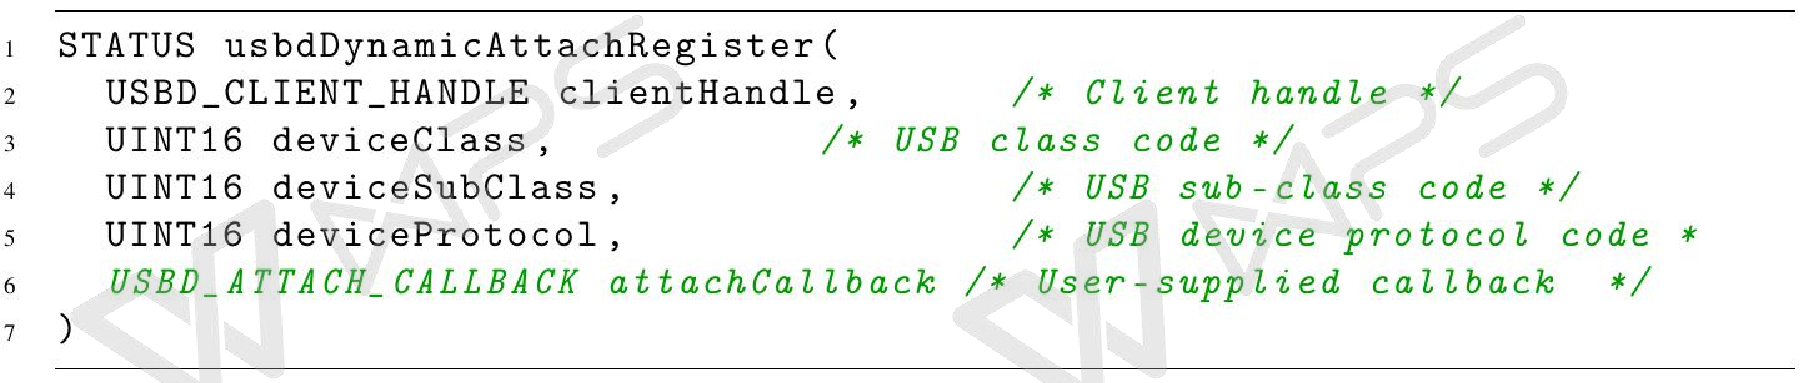
\includegraphics[width=1.0\textwidth]{./graphics/usbdDynamicAttachRegister.pdf}
\caption{热插拔注册函数}\label{fig:usbdDynamicAttachRegister}
\end{figure}


\subsection{设备的识别和初始化}

	设备的初始化工作需要在设备被我们的客户端驱动所识别之后才进行,在驱动初始化时我们注册好了热插拔的回调函数cp210xAttachCallback(),在
	回调函数中我们最先做的就是识别设备,识别完成之后再对其进行初始化,识别设备通过
	发送标准的USB设备请求命令来获取该设备的设备描述符,设备描述符当中包含有设备的类、子类、协议、厂商ID等信息,在VxWorks当中对USB设备描述符信息的定义如\autoref{fig:usdbDescriptorGet} 所示;

\begin{figure}[!h]
\centering
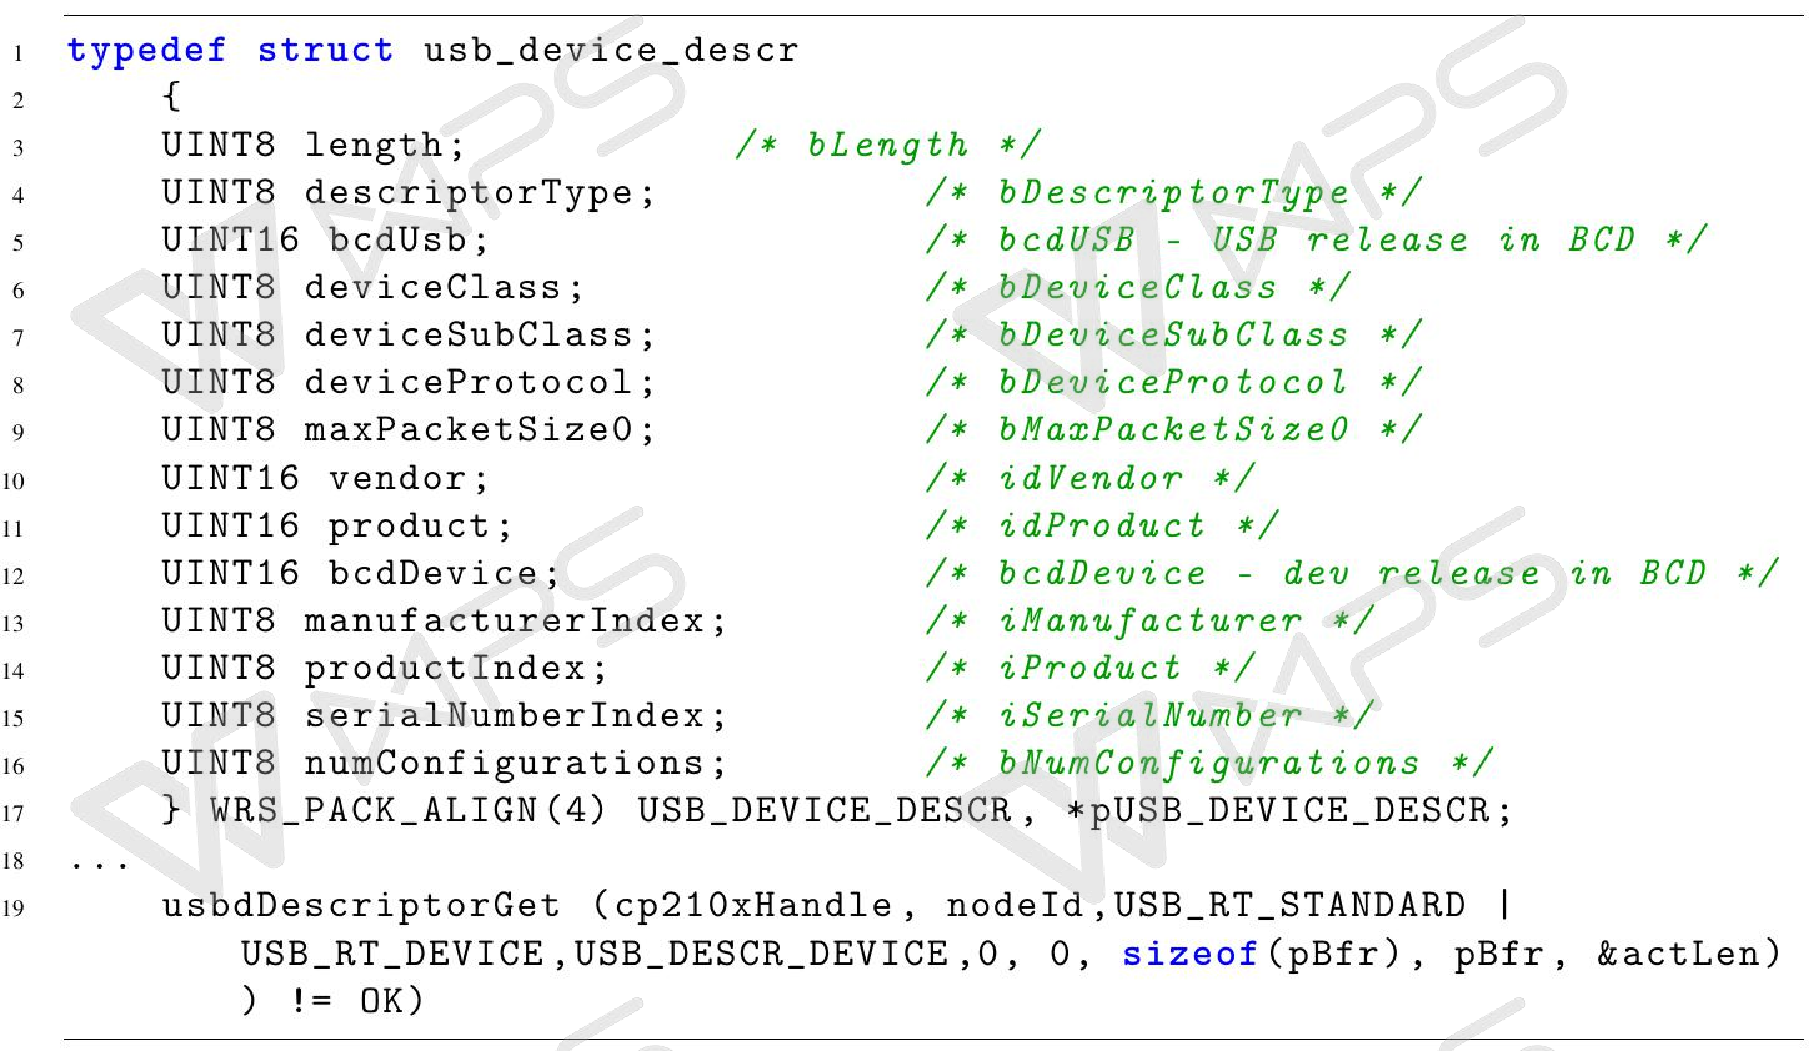
\includegraphics[width=1.0\textwidth]{./graphics/usdbDescriptorGet.pdf}
\caption{usb设备描述符信息结构}\label{fig:usdbDescriptorGet}
\end{figure}

VxWorks当中提供了usbdDescriptorGet()函数来获取设备描述符,该函数的三、四个参数用于指定所需要获取的描述的类型,对于此处我们需要获取的是设备的标准描述符,于是将其设置为USB\_ RT\_ STANDARD|USB\_ RT\_ DEVICE和USB\_ RT\_ DEVICE。
	我们将标准设备描述符的信息放在指向USB_DESCR_DEVICE类型的结构体指针pBfr当中,然后从中提取厂商ID和产品ID,我们将该驱动支持的设备的厂商ID和设备ID存储在一个全局的二维数组当中,然后通过遍历当前插入的设备的VID和PID是否在我们的数组当中来判断这个设备是否能够被我们的驱动所支持。设备识别的流程如\autoref{fig:device-recognize}所示,目前支持的设备的设备ID、产品ID的组合如\autoref{tab:目前支持的设备列表}所示。
\begin{figure}[!h]
\centering
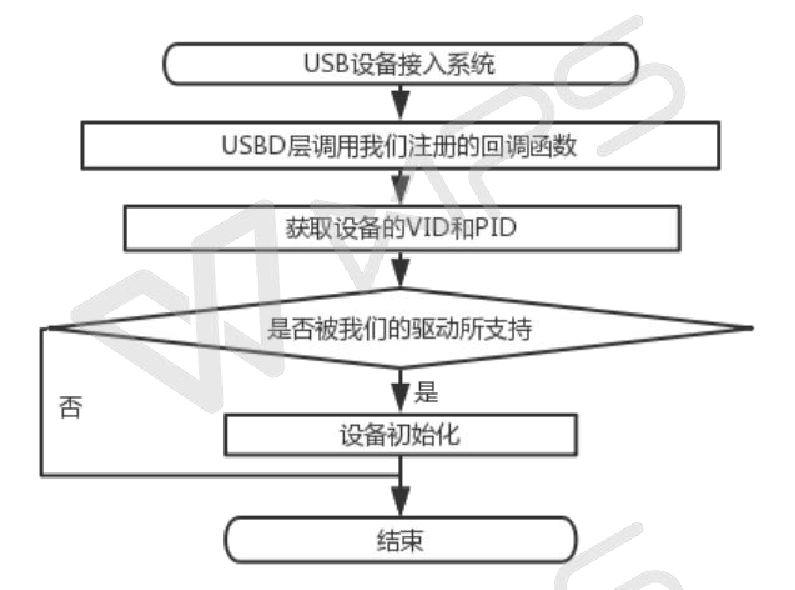
\includegraphics[width=1.0\textwidth]{./graphics/device-recognize.pdf}
\caption{设备识别流程图}\label{fig:device-recognize}
\end{figure}

\begin{table}[!h]
\centering
\begin{tabular}{|c|c|c|c|c|c|c|}
\hline
{\hei{PID}}&{0x045B}&{0x0471}&{0x0489}&{0x0489}&{0x10C4}&{0x10C4}\\ 
\hline
{\hei{VID}}&{0x0053}&{0x066A}&{0xE000}&{0xE003}&{0x80F6}&{0x8115}\\
\hline 
{\hei{PID}}&{0x10C4}&{0x10C4}&{0x10C4}&{0x10C4}&{0x10C4}&{0x2405}\\
\hline
{\hei{VID}}&{0xEA60}&{0x813D}&{0x813F}&{0x814A}&{0x814B}&{0x0003}\\
\hline
\end{tabular}
\caption{目前支持的设备列表}\label{tab:目前支持的设备列表}
\end{table}


	设备的初始化包括获取该USB设备的各种描述符信息。包括配置描述符信息、接口描述符信息、端点描述符信息。再通过所获得的这些信息来对设备进行接口进行配置、创建输入/输出管道。
	对于我们的USB口转串口设备还有一点特殊的地方在于它还需要配置串口的波特率、数据位、停止位、流控等信息,这是普通的USB设备所没有的。我们在此处将设备的波特率初始化为115200,数据位为8位,1个停止位,没有奇偶校验,没有流控。设备的初始化流程图如\autoref{fig:device-init}所示。
\begin{figure}[!h]
\centering
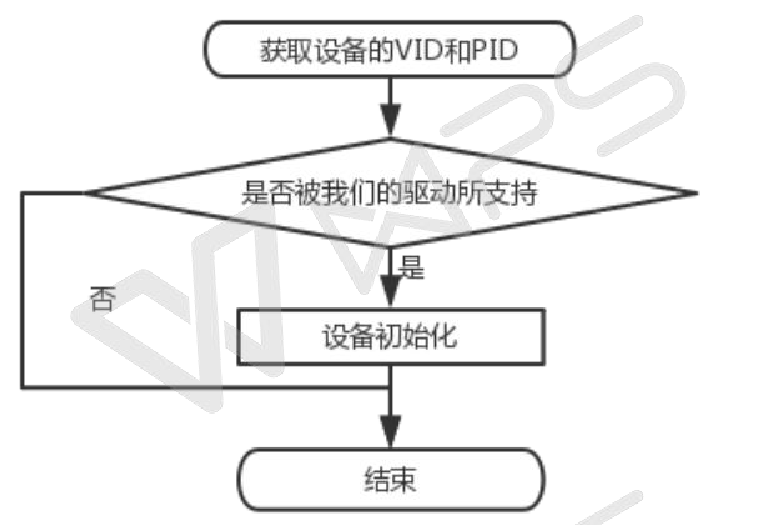
\includegraphics[width=15cm,height = 8cm]{./graphics/Dev-Init.pdf}
\caption{设备初始化流程图}\label{fig:device-init}
\end{figure}

这些描述符同样是通过usbdDescriptorGet()函数来发送设备的标准描述符命令来获取,在获取到
这些信息之后,通过usbdConfigurationSet()、usbdInterfaceSet()来配置设备,通过usbdPipeCreate()函数来设置设备的输入、输出管道,通过管道来连接设备的输入、输出端点。

	在驱动程序初始化完成之后我们会立即启动listenForInput()这个函数来注册一个设备输入的回调函数来监听设备的输入动作,当设备产生中断输入数据时,USBD层就会通知我们注册的这个回调函数。另外我们会立即执行一个发送操作的触发函数initOutPut(),当设备的输出缓冲区有数据时会立即执行数据的发送,这是我们的单设备驱动程序中一个特殊的流程。关于数据详细的传输和控制的过程我们会在\autoref{sec:设备的读写} 设备的读写部分介绍,设备识别和初始化的整个流程在回调函数中如\autoref{fig:SDevice-Driver-diagram-b}所示。
\begin{figure}[!h]
\centering
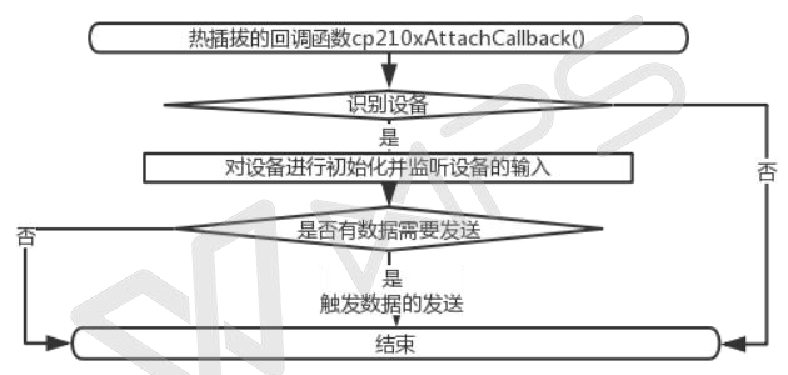
\includegraphics[width=1.0\textwidth]{./graphics/SDev-Drv-Diagram-b.pdf}
\caption{单设备回调函数流程}\label{fig:SDevice-Driver-diagram-b}
\end{figure}


\subsection{设备打开/关闭}	
	
	用户在使用一个设备之前必须先对这个设备进行打开,在这个过程当中通常而言底层驱动的响应函数会进行中断注册和使能设备工作配置等操作,但是对于我们的USB转串口驱动而言,我们不需要自己管理中断,USBD层会为我们进行中断的管理工作,而配置工作我们在设备的初始化时已经完成,因此此处我们的设备打开工作,只需要简单的记录设备被打开的次数并返回即可。设备的打开/关闭代码如下所示:
	
\lstset{language=C}
\begin{lstlisting}
LOCAL CP210X_DEV * cp210xDevOpen(DEV_HDR *pDevHdr, char *name, int flags,int mode)
{
  CP210X_DEV *pCp210xDev;
  pCp210xDev = (CP210X_DEV *)pDevHdr;	
  pCp210xDev->numOpen++;
  return (pCp210xDev);
}

LOCAL CP210X_DEV * cp210xDevClose(CP210X_DEV *pCp210xDev)
{
  --pCp210xDev->numOpen;
  return (pCp210xDev);
}

\end{lstlisting}

	cp210xDevOpen()函数用来承接系统的open()调用,它的第一个DEV\_ HDR类型的参数即是我们之前所说的必须是设备自定义结构的第一个成员,这个参数会由 I/O 子系统自动提供,I/O 子系统会根据驱动号寻址到对应驱动函数时,然后将对应的系统设备列表中存储的设备结构作为第一个参数来调用 cp210xDevOpen()。我们之后在使用的时候需要首先将这个 DEV\_ HDR 结构转换成我们的自定义结构 CP210X\_ DEV,但是我们也可以直接将第一个参数的类型设置为自定义结构类型,那么对于我们USB口转串口驱动,以上  cp210xDevOpen() 函数的调用原型就变为:LOCAL int cp210xDevOpen(CP210X\_ DEV *pCp210xDev, char *name, int flags,int mode)这并不会造成什么影响。
		
	第二个参数是设备名匹配后的剩余部分,注意不是我们传过来的设备名。VxWorks中使用最佳匹配的原则来匹配设备名,如我们打开一个设备"/ttyUsb/xyz",但是如果系统中并没有完全符合这个设备名的设备,而是只有名为"/ttyUsb/x"的设备,那么系统就会打开这个设备,而将匹配完成之后剩余的剩余的字符串"yz"传递给name。我们的应用中 open() 函数调用时的路径名应该与系统设备列表中的设备名是完全一致的,此处的 name 就会是一个空字符串,所以这个规则对于我们并没有什么影响。这是规则的主要用处在于处理文件系统层下的块设备,此时name可以指向块设备节点名后的子目录和文件名。

	第三,四个参数就是用户 open() 调用时传入的第二,三个参数,IO 子系统不会对他们进行任何更改,只是原封不动的转发给了 cp210xDevOpen() 函数。
	
	该函数的返回值有如下两种值:一个有效的CP210X\_ DEV结构指针表示 cp210xDevOpen 调用成功,ERROR 则表示 cp210xDevOpen()调用失败,I/O 子系统会根据返回的指针是否有效来决定返回一个文件描述符还是返回一个错误。cp210xDevOpen() 函数的返回值非常重要,这个指针将被 IO 子系统保存,用于其后对驱动中读写,控制函数的调用,这个返回的指针也会作为这些函数的第一个参数。
	
	设备的关闭和设备的打开操作是相反的操作,在关闭操作当中我们只需要对设备记录的打开次数进行减法操作即可。

\subsection{设备的读写}\label{sec:设备的读写}
	在open()操作成功之后,我们可以得到一个返回值,这个返回值就是设备的文件描述符,然后我们就可以使用这个文件描述符对设备进行read(),write()等操作。我们的USB口转串口驱动的读写函数原型如下:

\lstset{language=C}
\begin{lstlisting}
LOCAL CP210X_DEV * cp210xDevWrite(CP210X_DEV *pCp210xDev, char *buffer,UINT32 nBytes)
LOCAL CP210X_DEV * cp210xDevRead(CP210X_DEV *pCp210xDev, char *buffer,UINT32 nBytes)
\end{lstlisting}

由于我们特殊驱动程序的要求与普通流程下的驱动有所不同,其初始化方式比较特殊,对于数据的传输操作的流程也有相应的需求。我们在此需要对其数据流进行重新的设计。
	
	对于这个特殊流程的驱动程序,我们会在驱动程序初始化的时候就为其建立好输入输出缓冲区,而不是在设备初始化的时候为设备创建输入输出缓冲区,因为我们需要在设备还未连接的时候就能够打开设备,往设备的输出缓冲区中写入数据。特殊驱动程序的数据的输出操作会分为两个流程来进行。缓存空间的大小是以宏的方式定义在头文件当中的,方便以后改动,分别定义为:WRITE\_ BUFFER\_ SIZE和READ\_ BUFFER\_ SIZE。
	
	上层应用写入数据时会使用系统调用write(),该函数在VxWorks当中对应于我们驱动程序中的函数为cp210xDevWrite(),这个函数会接受write()发送过来的数据,并将其存入输出缓冲区中,并判断是否需要触发数据的发送操作。发送数据的触发操作只会在设备当前没有数据发送时完成,若调用write()时设备已经在发送数据,则只需要将数据存入缓冲区即可,设备发送完当前正在发送的数据之后会去判断缓冲区中是否还有数据,有数据则会继续发送。其流程图如\autoref{fig:SDevDataSend-A} 所示。

	
	设备在连接上系统并初始化之后就先查询缓冲区中是否存在数据,若存在数据则将其发送,
	一个数据包发送完成之后会再次去查询驱动的输出缓冲区中是否仍然有数据需要发送,若有数据要发送则继续发送,若没有则等待上层应用写入数据来触发数据的发送操作,其输出流程如\autoref{fig:SDevDataSend-B}所示 。

\begin{figure}[!h]
\centering
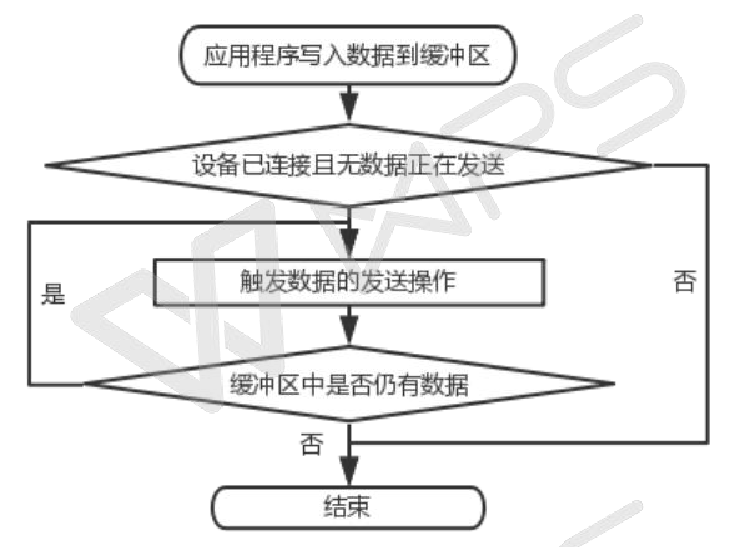
\includegraphics[width=12cm ,height=7cm]{./graphics/SDevDataSend-A.pdf}
\caption{write操作的输出流程}\label{fig:SDevDataSend-A}
\end{figure}

\begin{figure}[!h]
\centering
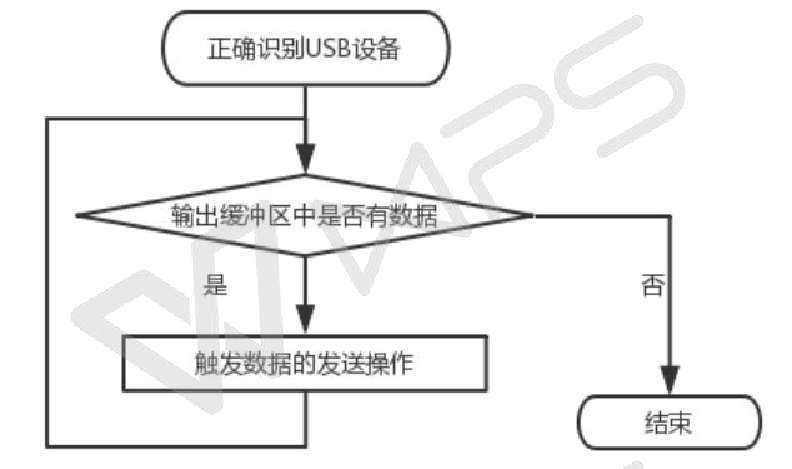
\includegraphics[width=12cm,height=7cm]{./graphics/SDevDataSend-B.pdf}
\caption{设备连接上系统时输出流程}\label{fig:SDevDataSend-B}
\end{figure}

	对于数据的输入操作,因为数据的输入是要依赖于实际的硬件的,不像输出操作一样存在“假”的输入。我们在设备的初始化完成之后我们会立即启动listenForInput()这个函数来注册一个设备输入的回调函数来监听设备的输入动作,当设备产生中断输入数据时,USBD层就会通知我们注册的这个回调函数,在这个回调函数中我们会处理设备输入的数据。
	
	在listenForInput()当中我们先创建好一个用来读取数据的USB IRP,在这个IRP当中我们注册回调函数为cp210xIrpCallback,获取IRP的超时时间为USB\_ TIMEOUT\_ NONE
	当有USB的输入管道当中有输入数据到来时USBD层会调用我们注册的回调函数来通知我们。在处理完一次的回调之后我们需要启动下一次的监听,因为每一次的IRP都是单次有效的,所以在cp210xIrpCallback()当中我们接收完这一次的IRP的数据并将其进行处理之后需要新建另一个IRP重新启动下一次的listenForInput()过程。


	因为我们的驱动的程序的主要功能就在于数据的传输,在数据的传输过程中对于缓冲区的设计和信号量的使用方式直接影响到我们的驱动程序性能,因此有必要对这两部分再进行详细的描述。
	
\subsubsection{环形缓冲区的设计和控制}
		
  应用程序、设备驱动和环形缓冲区的关系如\autoref{fig:设备数据缓冲}所示,通过环形数据缓冲,我们可以解决速度匹配的问题和数据丢失的问题,应用程序也无需阻塞等待设备的空闲,只需将数据发送到我们的缓冲区中即可。
  
\begin{figure}[!h]
\centering
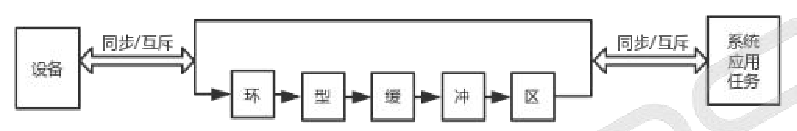
\includegraphics[width=.9\textwidth]{./graphics/Dev-Data-Buf.pdf}
\caption{设备数据缓冲}\label{fig:设备数据缓冲}
\end{figure}

 
	我们使用循环队列实现的来实现环形缓冲区,由于计算机的内存是线性地址空间,因此从逻辑上实现环形缓冲区时通常需要4个指针:
	 \begin{itemize}
	 \item 在内存中实际开始位置的指针;
	 \item 在内存中实际结束位置的指针,或者缓冲区的长度,由于我们已经在驱动中定义了缓冲区的长度为WRITE\_ BUFFER\_ SIZE和READ\_ BUFFER\_ SIZE,所以这个指针我们不再需要;
	 \item 存储在缓冲区中的有效数据的开始位置(读指针);
	 \item 存储在缓冲区中的有效数据的结束位置的指针(写指针)。
	 \end{itemize}
	
	当数据元素插入或者是删除时,我们不需要移动其余的数据元素存储位置,只需要移动队头和队尾指针即可。在设备初始化时,将设备的环形缓冲区清空,队头指针和队尾指针均设为 0,当缓冲区中接收到一个数据时,将此数据保存到队尾的位置并将队尾指针加1,当缓冲区中取走一个数据时,我们将队头指针减一。

	无论是对于读缓冲区还是写缓冲区,我们都需要解决的一个问题是当循环缓冲区中的数据已经满了之后,再有数据需要进入到缓冲区当中时,我们怎么进行处理,此处我们选择的策略是遵循先进先出的原则来覆盖数据。这样操作的好处是可以防止最新的数据丢失,而老的数据可能已经失去了时效性。

	对于输入缓冲区,我们使用一个读互斥信号量cp210xReadMutex和一个读二进制信号量ReadblockSem来进行缓冲区的控制,cp210xReadMutex的作用保证对读缓冲区的正确访问顺序,ReadblockSem的作用是用于对上层读任务和底层驱动的写任务进行同步。在使用ReadblockSem时我们会设置一个超时时间TIMEOUT,当时间超过时semTake()操作就会返回一个错误,我们上层读取任务此时就会得到一个错误返回,说明无法读取到数据。
	当需要读取 nbytes 个字节而缓冲区内的字节不够时,read就会阻塞,直到超时返回或者USBD层通知你有新的数据到来时再继续进行读操作。同时也在驱动中启动了一个计时器,如果在计时器时间到了之后,还未能满足需要读取的字节数,则退出本次读写操作,返回当前已处理的字节数。

\lstset{language=C}
\begin{lstlisting}
cp210xDevRead(...)//上层应用读取任务
{
...
	semTake(cp210xReadMutex,WAIT_FOR_EVER)	
	if(available == 0)
	{
		semGive(cp210xReadMutex)
		//等待缓冲区写入数据,当底层往缓冲区中写入数据时会释放ReadblockSem
		status = semTake(ReadblockSem,TIEMOUT);
		if(status == ERROR)
			return ERROR;
			
		semTake(cp210xReadMutex,WAIT_FOR_EVER)
	}
	copy_from_readBuf; /*从缓冲区读取数据*/
	semGive(cp210xReadMutex)
	...
}

cp210xIrpCallback(...)//底层从硬件接收数据
{
...
	semTake(cp210xReadMutex,WAIT_FOR_EVER)
	if(available == 0)//缓冲区中没有数据,则释放一次ReadblockSem
		semGive(ReadblockSem);
	copy_to_readBuf()//向读缓冲区中写入数据
	semGive(cp210xReadMutex);
...
}
\end{lstlisting}  


	对于输出缓冲区,我们使用一个写互斥信号量cp210xWriteMutex来进行缓冲区的读写控制,由于我们这个特殊的驱动程序在往外输出数据时只需要将数据输出到了缓冲区的即可,不管实际的设备是否连接,因此我们不需要使用二进制信号量来进行上层写任务和底层读任务之间的同步操作。此时设备如果连接在系统上则会触发数据的发送操作,若设备没有连接在系统上,那么设备在连接上之后会自动的进行一次判断缓冲区中是否有数据的操作,有数据则触发发送操作。部分关键代码如下:

\lstset{language=C}
\begin{lstlisting}
cp210xDevWrite(...)//上层应用写任务
{
...	
  semTake(cp210xWriteMutex,WAIT_FOR_EVER);
  copy_to_writeBuf; /*从缓冲区读取数据*/
  semGive(cp210xWriteMutex);
...
}

initOutPut()//底层从缓冲区读取数据写入设备
{
...
  semTake(cp210xWriteMutex,WAIT_FOR_EVER)
  if(available == 0)
  {
	semGive(cp210xWriteMutex);
	return;
  }	
  copy_from_writeBuf()//从输出缓冲区中取出数据发送
  initOutIrp();//构建数据发送IRP
  semGive(cp210xWriteMutex);
  ...
}
\end{lstlisting}  





\subsection{设备的控制操作}
	设备控制操作用于对设备的某一些工作行为进行再配置,可供执行的再配置类别随着设备类型的不同而不同,操作系统当中通常会一种类型的设备的某一组共同属性作为一个配置选项,比如波特率再配置就是串口的一个标准属性,而一般的USB设备是不具有该属性的。但是这只是一个约定,并不是所有的设备都必须要完全对照这一准则,底层驱动也可以根据自己的实际需要来对这些再配置属性进行选择,我们可以选择只实现某一些再配置参数,也可以根据具体情况对某一个再配置选项进行响应,设备控制函数给用户控制设备提供方便的同时也对底层设备的实现提供了极大的方便性。
	
	对于我们的USB转串口驱动而言,其属于一个特殊的设备,没法归入操作系统的已经分好类的设备当中,我们需要实现一些非约定的配置属性,如配置波特率、流控、数据位等等非USB所属的配置选项。
	我们将USB转串口驱动特定的参数定义在一个头文件当中,而后将这个头文件提供给用户程序,当用户对设备进行操作时,其包含这个头文件,使用其中定义的特定参数对设备进行控制。IO 子系统不会对用户调用的ioctl()函数做任何的改变,只会将用户使用的选项参数或者控制命令传递给我们的cp210xDevIoctl()函数,然后由这个函数完成对选项参数或控制命令的解释和使用。
设备控制函数原型如下:
\lstset{language=C}
\begin{lstlisting}
LOCAL CP210X_DEV * cp210xDevIoctl(CP210X_DEV *pCp210xDev, int request, void *someArg )
\end{lstlisting}

对于我们的 USB转串口驱动,在实际使用中,再配置参数和命令有很多,但是目前我们只提供设备的波特率、数据位、校验位、流控的参数和命令。这些控制对于普通的USB设备而言是没有的,他们在定义上属于USB的厂商自定义请求,在我们的驱动程序的cp210xDevIoctl()函数当中我们会使用switch语句来对请求类型进行分类,所有的请求最后都要使用usbdVendorSpecific()函数来发送USB的厂商自定义请求,该函数的原型如\autoref{fig:usbdVendorSpecific}所示。


\begin{figure}[!h]
\centering
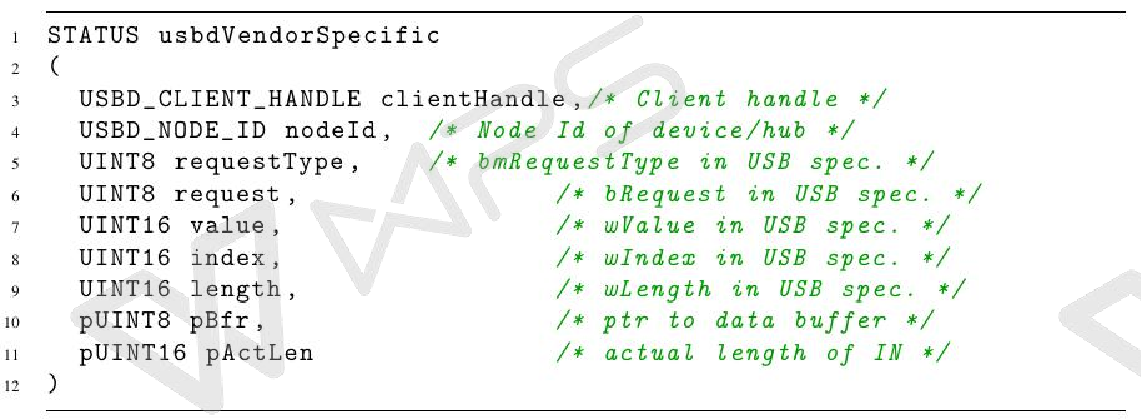
\includegraphics[width=1.0\textwidth]{./graphics/usbdVendorSpecify.pdf}
\caption{usbdVendorSpecific()}\label{fig:usbdVendorSpecific}
\end{figure}

其中第三个参数是请求类型,表示该类型是从主机到设备的,还是从设备到主机的,有四种类型,分别是REQTYPE\_ HOST\_ TO\_ INTERFACE(0x41),REQTYPE\_ INTERFACE\_ TO\_ HOST(0xC1),REQTYPE\_ HOST\_ TO\_ DEVICE(0x40),REQTYPE\_ DEVICE\_ TO\_ HOST((0xC0)),第四个参数是具体的请求,对于我们的设备而言能响应的部分主要请求如\autoref{fig:部分厂商自定义请求} 所示。

\begin{figure}[!h]
\centering
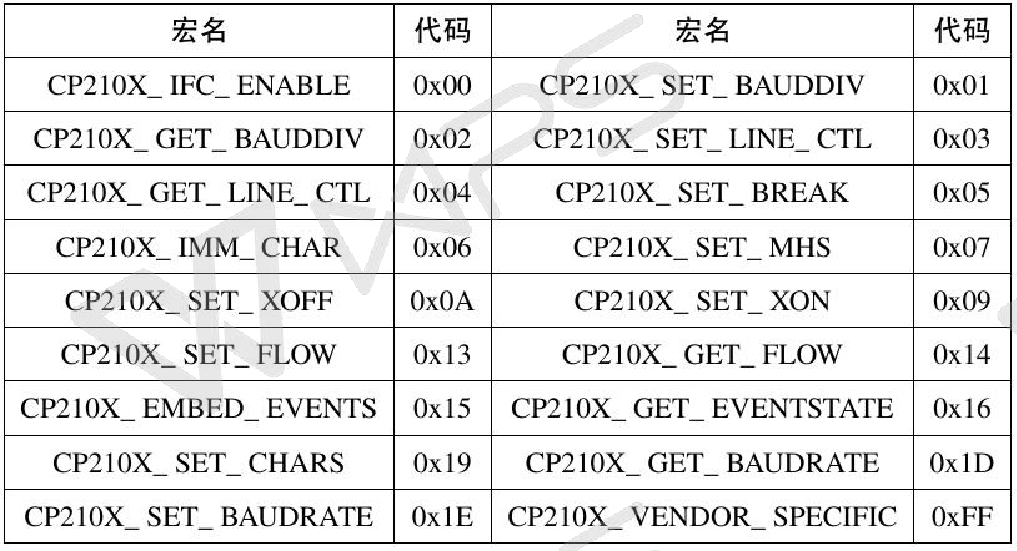
\includegraphics[width=12cm ,height=7cm]{./graphics/vendorSpecify.pdf}
\caption{部分厂商自定义请求}\label{fig:部分厂商自定义请求}
\end{figure}


\subsection{驱动卸载}
	在驱动的卸载函数当中我们需要完成驱动的反注册,包括注销向USBD层的注册和向系统设备表的注册,同时还需要销毁具体的设备所占用的各种资源。
	
	在单设备驱动的注销函数中我们应该首先对驱动的热插拔回调函数进行注销,这样就可以阻止对此后再接入系统上的设备进行响应,之后应该因此注销USBD客户端、系统设备表、系统驱动表,然后再清理驱动的全局资源和设备对应的资源。若此时由设备连接在系统上且有数据正在发送,那么应该等待设备当前正在发送的数据发送完之后再清理设备对应的资源,其流程如\autoref{fig:SDevUninit}所示。
\begin{figure}[!h]
\centering
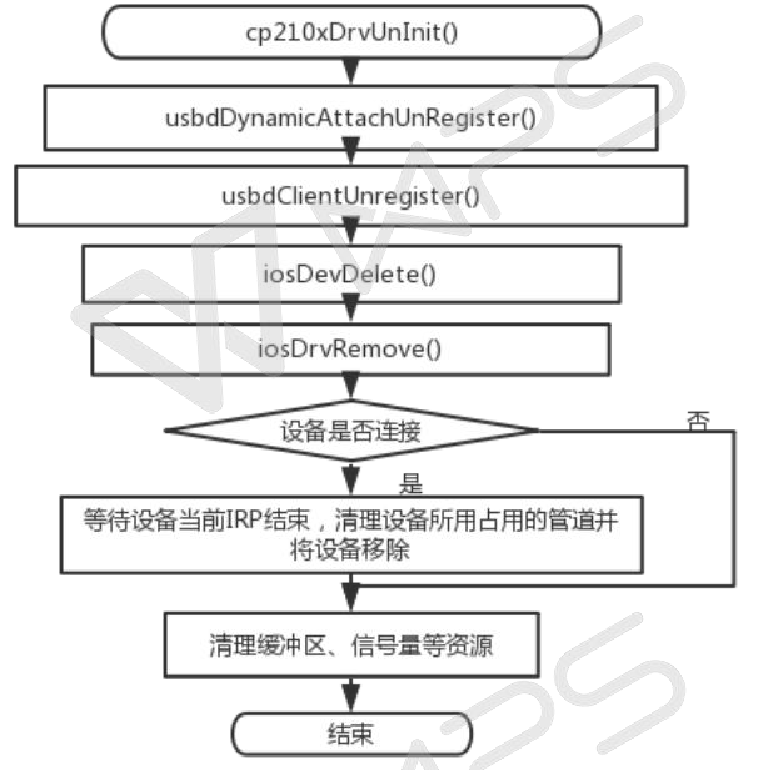
\includegraphics[width=12cm ,height=10cm]{./graphics/SDevUninit.pdf}
\caption{单设备驱动注销流程}\label{fig:SDevUninit}
\end{figure}
	

	在驱动的初始化函数cp210xDrvInit()当中我们使用了 iosDrvInstall() 函数向 IO 子系统注册我们的驱动,在wind中也提供了另外一个相反作用的函数iosDrvRemove()注销我们的驱动。该函数调用原型如\autoref{fig:iosDrvRemove}所示。
	
\begin{figure}[!h]
\centering
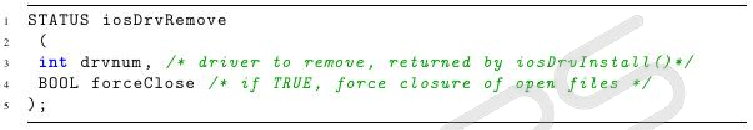
\includegraphics[width=1.0\textwidth]{./graphics/iosDrvRemove.pdf}
\caption{iosDrvRemove()}\label{fig:iosDrvRemove}
\end{figure}

该函数的第二个参数指定是否对驱动程序进行强制性的卸载,并将所有与此驱动有关的文件描述符关闭。如果强制关闭,则 IO 子系统将遍历系统文件描述符表,检查每个描述符对应结构中的驱动号是否等于要卸载驱动的驱动号,如果相同,则调用这个驱动的 close 实现函数进行关闭,同时释放文件描述符表中该表项,此时用户层的文件句柄将自动失去功效,如果用户其后使用这个文件描述符,将直接得到一个错误返回。




至此,我们已经完成了该特定需求下的USB口转串口驱动程序的所有组成部分的设计和实现。

\section{通用多设备驱动的实现}
	多设备驱动与特殊需求的单设备驱动最明显的不同之处在于整个驱动程序的启动流程不一样,其次需要支持多设备,要在识别设备后给每一个设备分配一个设备名,并加入到系统设备表当中,然后需要给每一个设备初始化自己的设备自定义结构体,多设备驱动的具体设计如下文所述。


\subsection{设备的自定义结构体}

在多设备的自定义结构体当中除了要保存和单设备结构体当中一样的设备的配置、管道、端点地址等信息之外,我们还需要保存每一个设备的读写缓冲区的基地址和头尾指针。除此之外我们使用了一个链表devHdrLink来链接接入系统上的该驱动支持的USB设备,每次检测到新设备时我们可以通过将新添加的设备增加到这个链表当中,之后可以通过nodeId来从多个设备中定位我们的设备是否存在,若不存在则给该设备分配一个设备名。
多设备的驱动自定义结构体的部分定义如下所示:
\lstset{language=C}
\begin{lstlisting}
typedef struct cp210x_dev
{
  DEV_HDR cp210xDevHdr; /*must be first field*/
  LINK 	devHdrLink; /*linked list of  devhdr structs*/
  ...
  
  char *writeBuf;
  int writeFront;
  int writeRear;
  char *readBuf;
  int readFront;
  int readRear;
} CP210X_DEV, *pCP210XDEV;
\end{lstlisting}

	

\subsection{驱动初始化}
	与单设备驱动程序中的驱动初始化流程不同的是,对于多设备驱动在初始化的时候我们不需要先注册设备和初始化输入输出缓冲区,在多设备驱动初始化的时候我们只需要将驱动程序注册到系统驱动表即可,不需要将其注册系统设备表,注册系统设备表需要在设备初始化时完成,除此之外我们还需要将驱动向USBD层进行注册多设备下的驱动初始化流程如\autoref{fig:MDevice-Driver-diagram-a}所示。

	
\begin{figure}[!h]
\centering
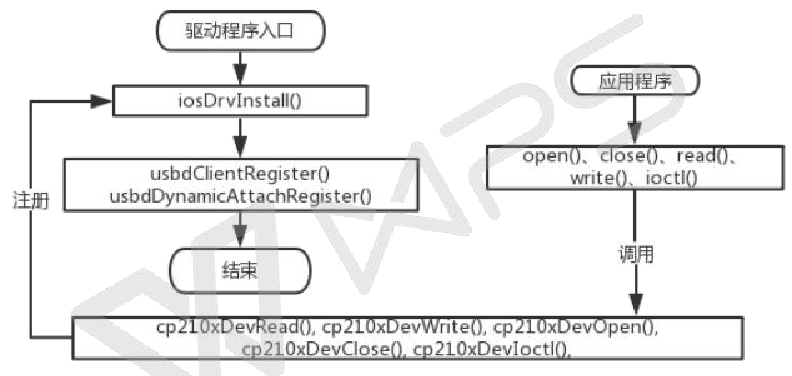
\includegraphics[width=1.0\textwidth]{./graphics/MDev-Drv-Diagram-a.pdf}
\caption{多设备驱动初始化流程}\label{fig:MDevice-Driver-diagram-a}
\end{figure}


\subsection{设备的识别和初始化}

设备的初始化工作同样是从设备插入系统之后的回调函数开始的,在驱动初始化时我们注册好了热插拔的回调函数cp210xAttachCallback(),和单设备驱动中的识别过程一样,我们通过发送标准的USB设备请求命令来获取该设备的设备描述符,然后通过设备的VID和PID来识别设备,多设备驱动中设备和识别和初始化流程如\autoref{fig:MDevice-Driver-diagram-b}所示 。

\begin{figure}[!h]
\centering
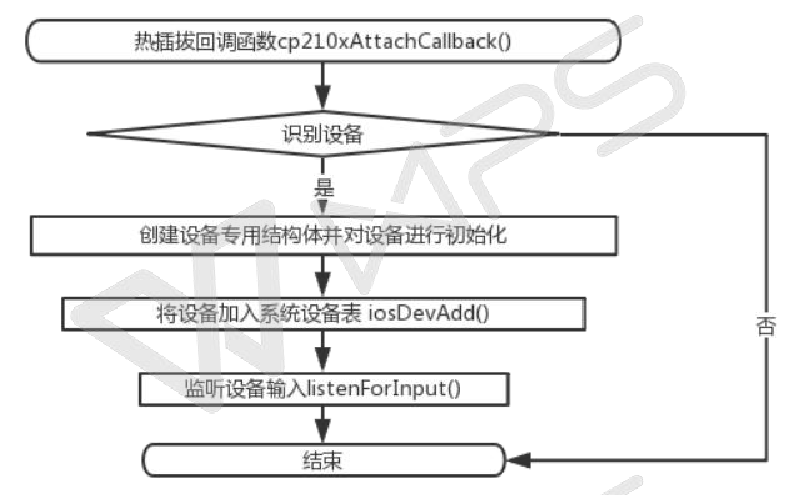
\includegraphics[width=1.0\textwidth]{./graphics/MDev-Drv-Diagram-b.pdf}
\caption{多设备回调函数流程}\label{fig:MDevice-Driver-diagram-b}
\end{figure}

	比较单设备驱动中设备初始化(如\autoref{fig:SDevice-Driver-diagram-b}所示)和多设备驱动中设备初始化(如\autoref{fig:MDevice-Driver-diagram-b}所示)的过程,我们可以看出在驱动注册过程中两者的区别,在单设备驱动的设备初始化中我们无需在完成设备添加到系统设备表的过程,因为这一过程已在驱动初始化当中完成。而多设备驱动中设备初始化的过程需要识别每一个设备并给支持的设备分配一个设备名和设备的自有资源,然后再将该设备添加到系统设备表当中。
	在设备创建时我们会通过判断已连接设备的个数来决定当前设备所采用的设备名,使用的设备名诸如“/UsbSerial/0”,“/UsbSerial/1”...。



\subsection{设备的打开/关闭}
	通用多设备驱动相对于我们上述的单设备驱动而言在打开/关闭操作的不同之处在于需要在打开或者关闭之前判断设备是否仍然连接在系统上,因为设备可能未连接在系统上或者在open()之后已经拔出了设备。
	因为对于通用多设备驱动而言不存在“假”的设备,不能在设备未连接时往缓冲区当中写数据,所以我们需要在执行打开/关闭操作的函数内首先判断设备是否仍然处于连接状态。除此之外只需要记录下设备打开和关闭的次数即可。
	

\subsection{设备的读写}
	
	在多设备的驱动内部我们会为每一个连接到系统上的设备建立一个输入循环缓冲区和一个输出循环缓冲区,分别用于从设备接收输入数据和接收上层应用的输出数据。每个设备的缓存空间的大小作为以宏的方式定义在头文件当中,方便以后改动,分别定义为:WRITE\_ BUFFER\_ SIZE和READ\_ BUFFER\_ SIZE。
		
	对于通用多设备的写操作,与单设备驱动的写操作不同的是在设备连接上时,没有一个自动发送缓冲区的数据的过程,因为对于多设备驱动而言在设备连接上之前是不可能往缓冲区中写入数据的,只有在上层应用调用write()操作之后才会往该设备的缓冲区中写入数据,并触发数据的发送操作。其基本流程如\autoref{fig:MDevDataSend}所示。

\begin{figure}[!h]
\centering
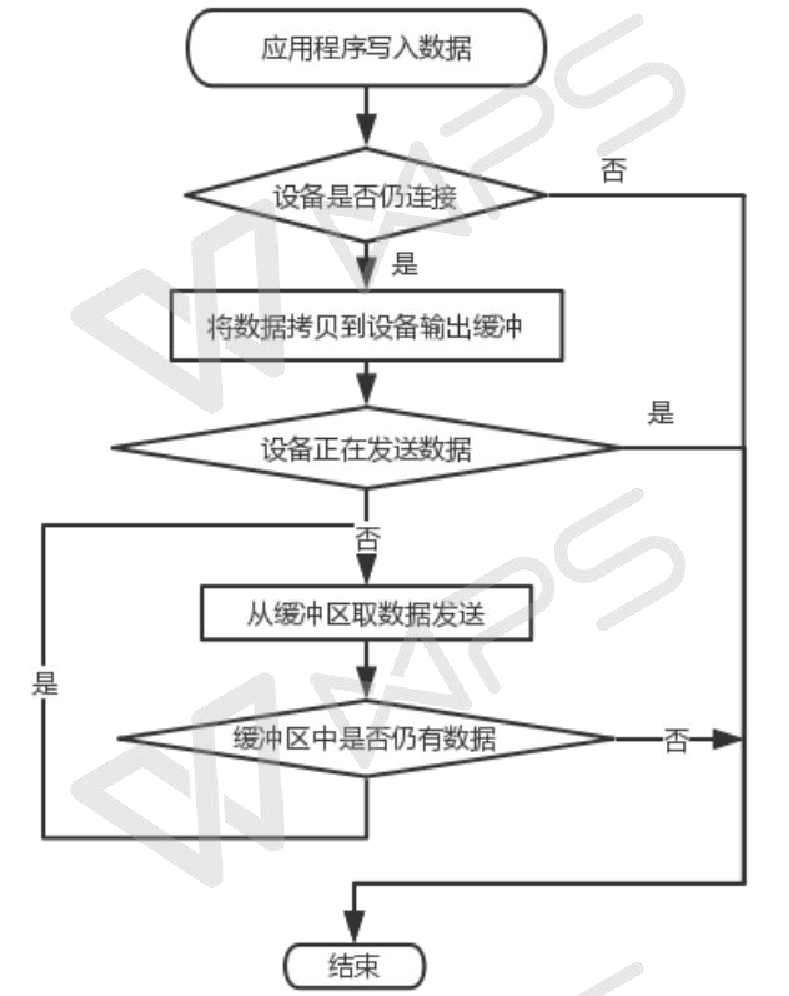
\includegraphics[width=13cm , height=10cm]{./graphics/MDevDataSend.pdf}
\caption{多设备驱动数据发送逻辑图}\label{fig:MDevDataSend}
\end{figure}

对于上层应用的write()操作,我们首先判断该设备是否仍然处于连接状态,若设备不处于连接状态则直接返回错误即可,若正处于连接状态则将数据拷贝到该设备的发送缓冲区,若当前设备正在进行数据的发送,则直接结束即可,若当前设备没有数据正在发送则触发数据的发送操作,设备在发送完一次的数据包之后会检查缓冲区中是否仍然有数据,若有数据则继续发送,若没有数据了则结束。
	
	
	同样我们在多设备驱动下使用一个互斥信号cp210xWriteMutex对输出缓冲区进行控制,首先在写入数据的时候需要进行互斥写,因为此时设备有可能正在从缓冲区当中取数据进行输出操作,那么这时写入输出缓冲区就需要等待,否则可能会造成缓冲区的混乱,造成输出结果与输入数据不一致。当设备输出从缓冲区拷贝完成之后就会释放互斥信号量,此时写入操作就可以往输出缓冲区中写入数据。

	
	多设备下的数据的输入  操作的实现方式与单设备下的相同, 都是在设备接入系统之后就向USBD层注册一个回调函数和一个IRP接收设备的输入,即listenForInput (),这个函数的实现与单设备驱动当中的一致,然后在cp210xIrpCallback()函数当中处理设备的输入,并启动下一次的listenForInput (),



\subsection{驱动卸载}
	在多设备驱动当中驱动的初始化流程与所设备中的不同,此时多设备驱动的卸载流程与单设备的驱动卸载流程也有一些相异之处,我们多设备驱动的卸载流程如\autoref{fig:MDevUninit}所示。与多设备驱动不同之处在于此处为每一个连接在系统上的设备执行iosDevDelete()操作,因此在单设备驱动中设备名是固定的,在驱动初始化时已经加载到系统设备表当中。而多设备驱动中设备名是动态的,需要根据插入系统中的设备数来决定,需要在设备初始化完成之后才将其加入系统设备表当中,在清理设备所占有的资源的时候同样要先等待设备当前的数据传输完成之后再清理。
	
	
\begin{figure}[!h]
\centering
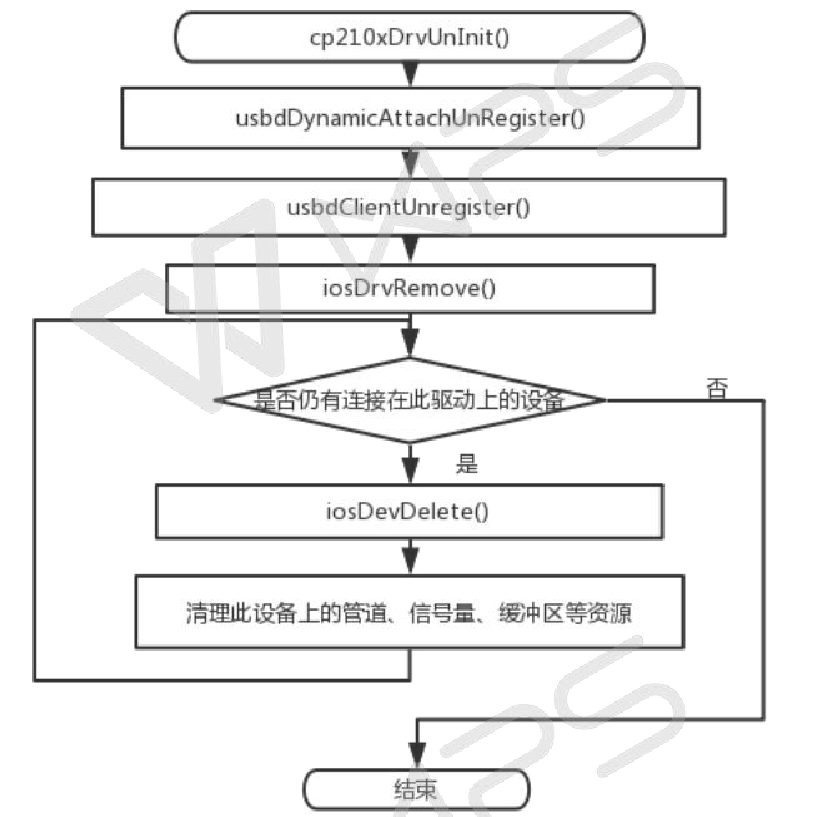
\includegraphics[width=12cm ,height=10cm]{./graphics/MDevUninit.pdf}
\caption{多设备驱动注销流程}\label{fig:MDevUninit}
\end{figure}


	对于多设备情况下的驱动的设备控制与单设备下的相比不需要做改变即可完成,此时操作的设备就是我们使用设备名打开的那个设备,IO子系统会将设备名映射到该设备所对应地驱动。





\section{小结}
	本章首先介绍了我们的USB口转串口驱动的设计想法,包括VxWorks下进行USB驱动开发的层次结构,USB口转串口所使用转换器的选择和对其进行开发工作所必须的知识。接下来我们讲解了我们的驱动程序的具体的设计和实现的方式,包括驱动中要实现的模块,每个模块的功能是什么,如何实现这些模块。





\clearpage
\chapter{应用层程序接口封装}
	由于VxWorks从6.x开始引入了RTP(VxWorks Real Time Process Project)模式,RTP模式对用户而言增加了更多的权限限制,对于应用程序而言也有了较为明显的内核态和用户态的区别,数据需要在内核态和用户态之间进行内存拷贝,执行效率有所降低,不过对于现代CPU的速度而言,这点速度的降低并不是很明显,不过对于实时性要求很高的应用而言还是应该使用task的模式来构建程序。RTP模式的优点是应用程序之间互相独立,这有利于增强内核的稳定性和安全性。对于我们而言其最直接的影响就是在RTP模式下有很多的内核函数都不能够再直接进行调用,而是需要使用封装的接口调用。
	
	
\section{应用层接口模块设计}

	应用层的接口包括两个部分:一是标准输出重定向接口的设计,目的是在程序运行期间直接调用标准输出函数时就能够将输出信息通过我们的串口输出出去,但是这个标准输出输出的信息不是格式化的信息。二是Log接口函数,通过调用这个接口函数可以将调试信息格式化输出,输出信息会自动包括调试的级别、产生的时间、所处的文件、行号等信息,便于对调试信息进行分析。

主要的模块包块以下两个:
\begin{itemize}
\item \hei{ResetStdOut():} 提供给用户选择是否需要重定向标准输出,若参数为1则将标准输出进行重定向,若参数为0,则关闭标准输出重定向,恢复到之前的标准输出。




\item \hei{Log接口函数:} 提供封装的不同级别的Log调试接口,包括LogE(表示错误信息)、LogD(表示详情信息)、LogW(表示警告信息)、LogI(表示)
\end{itemize}

由于RTP模式的引入,在这种模式下对于我们的标准输出重定向接口而言,其实现方式与task模式下存在一些差别,在task模式下我们需要使用VxWorks封装好的ioTaskStdSet()函数来实现重定向,而在RTP模式下我们无法使用,只能寻找其他的解决办法,在此处我们使用的是dup2()/dup()来实现。


\section{Log协议的设计}

对于Log接口函数我们设计为其为设计了专用的输出协议,如\autoref{fig:Log协议字段} 所示,在协议中包含了五种不同的输出级别,分别用LogE(表示错误信息)、LogD(表示调试信息)、LogW(表示警告信息)、LogI(表示详情信息)、Logo(表示其他信息)。同时我们还在协议中包含了一些调试信息所需要的关键信息字段,包括任务ID字段、任务名字段、文件名字段、行号字段、时间字段。
\begin{figure}[!h]
\centering
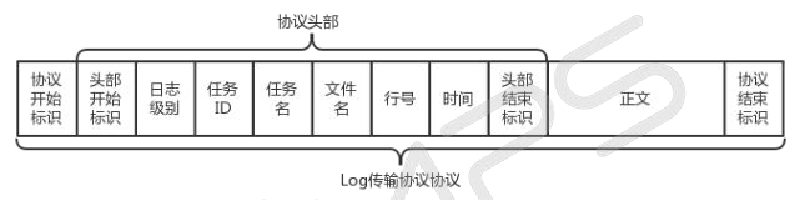
\includegraphics[width=.9\textwidth]{./graphics/Logxieyi.pdf}
\caption{Log协议字段}\label{fig:Log协议字段}
\end{figure}

我们为调试信息制定的协议格式为:\backslash 03\backslash 03<L=日志级别;PN=任务ID;P=任务名;F=文件名;N=行号;T=时间>contents\backslash 04\backslash 04\\
其中各部分的含义如下:

\begin{itemize}
\item \textbf{\backslash 03\backslash 03}:表示自定义的Log协议的数据包的开始;

\item \textbf{<}:表示自定义的Log协议数据包头部的开始;

\item \textbf{L}:表示日志的级别,我们在此将日志分为五个级别:
	\begin{itemize}
	\item e:表示error;
	
	\item w:表示warning;
	
	\item i:表示info;
	
	\item d:表示debug;
	
	\item o:表示其他信息。
	\end{itemize}
	
\item \textbf{PN}:此处的内容是输出该条调试信息的任务的任务ID;

\item \textbf{P}:此处的内容是输出该条调试信息的任务的任务名;

\item \textbf{F}:此处的内容是输出该条调试信息的任务所在的文件名;

\item \textbf{N}:此处的内容是该调试信息语句所在的文件的行号;

\item \textbf{T}:此处的内容是这条调试信息被输出时候的系统时间;

\item \textbf{>}:表示自定义的Log协议数据包头部的结束;

\item \textbf{contents}:这个部分是调试信息的正文部分。

\item \textbf{\backslash 04 \backslash 04}:表示自定义的 Log 协议数据包的结束。

\end{itemize}\\


\section{标准输出重定向接口的实现}
	由于标准输出的重定向无法在RTP模式和task模式下使用同一种方法来实现,于是我们使用了两种方法来分别实现RTP模式和task模式下的标准输出重定向。
\subsection{RTP模式下标准输出重定向}
	RTP模式下的标准输出重定向流程如\autoref{fig:rtp-printf-reset}所示。
\begin{figure}[!h]
\centering
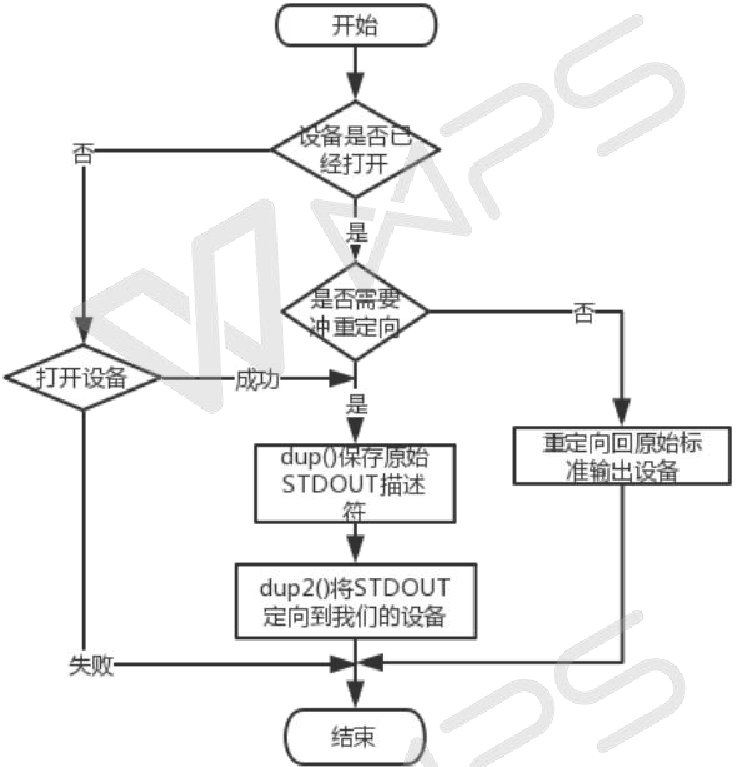
\includegraphics[width=0.7\textwidth , height=10cm]{./graphics/RTP-STDOUT-RESET.pdf}
\caption{RTP模式下标准输出重定向流程图}\label{fig:rtp-printf-reset}
\end{figure}


在RTP模式下使用dup/dup2函数来实现标准输出的重定向,首先需要指定一个需要重定向到的设备,然后判断该设备是否已经打开,若设备已打开则判断其是要重定向到远程终端还是重定向到本地的标准输出,重定向到远程设备时需要先使用dup来保存原始的标准输出,方便之后重定向会本地的标准输出,然后使用dup2将标准输出重定向到远程设备,若设备未打开则先将指定的重定向设备打开再执行重定向操作。

dup2函数的原型为:
\lstset{language=C}
\begin{lstlisting}
int dup2(int oldfd, int newfd);
\end{lstlisting}\\
dup2()用于复制描述符oldFd到newFd的,其中oldFd是要被复制的文件描述符,newFd是制定的新文件描述符,如果newFd已经打开,它将首先被关闭。如果newFd等于oldFd,dup2会返回newFd,但是不会关闭它。函数调用成功时会返回新的文件描述符,所返回的新的描述子与参数oldFd给定的描述符字引用同一个打开的文件,即共享同一个系统打开文件表项。函数调用失败时会返回-1并设置errno。

\subsection{task模式下标准输出重定向}
在task模式下无法使用dup()/dup2()函数来进行标准输出的重定向,在task模式下VxWorks有专用的标准输出接口ioTaskStdSet(),我们在此模式下只能使用这个接口来实现重定向,task模式下的标准输出重定向如\autoref{fig:task-printf-reset}所示。

\begin{figure}[!h]
\centering
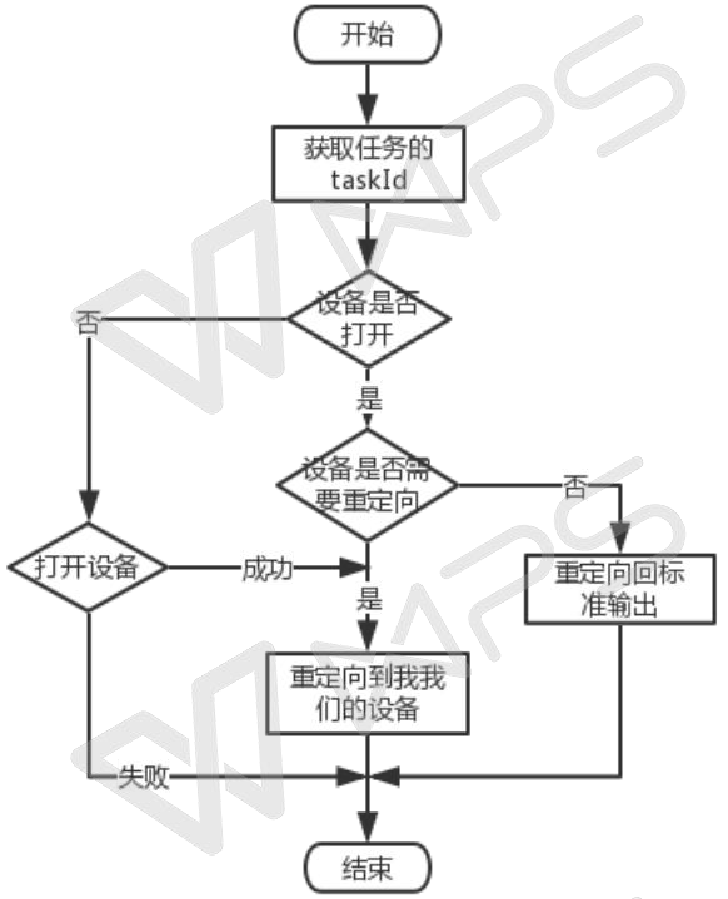
\includegraphics[width=0.7\textwidth ,height=10cm]{./graphics/TASK-STDOUT-RESET.pdf}
\caption{task模式下标准输出重定向流程图}\label{fig:task-printf-reset}
\end{figure}

ioTaskStdSet()是VxWorks专门用来进行任务级的重定向的函数。其函数原型为:
\lstset{language=C}
\begin{lstlisting}
void ioTaskStdSet(int taskId, int stdFd, int newFd);
\end{lstlisting}\\
在VxWorks中每一个任务都有一个数组taskStd,用于表明这个任务的标准输入、标准输出、标准错误,函数ioTaskStdSet()的功能就是将特定任务的标准描述符重定向到newFd,newFd需要是一个文件或者设备的描述符。


\section{Log接口的实现}
	Log接口函数用于完成标准格式的log的输出,使用时只需要调用LogE()、LogW()、LogI()、LogD()、LogO(),这几个接口均为宏定义,定义在usb\_ logWrite.h当中,在使用时需要包含该头文件,作用是获取log协议所需要的部分信息,其代码如下所示:
\lstset{language=C}
\begin{lstlisting}
#define LogE(format, ...) usb_logWrite('e',__FILE__,__LINE__,format,##__VA_ARGS__)

#define LogD(format, ...) usb_logWrite('d',__FILE__,__LINE__,format,##__VA_ ARGS__)

#define LogI(format, ...) usb_logWrite('i',__FILE__,__LINE__,format,##__VA_ ARGS__)

#define LogW(format, ...) usb_logWrite('w',__FILE__,__LINE__,format,##__VA_ ARGS__)

#define LogO(format, ...) usb_logWrite('o',__FILE__,__LINE__,format,##__VA_ ARGS__)

extern int usb_logWrite(char level,char *fileName, int lineNum, const char * format, ...);
\end{lstlisting}
LogE(),LogW(),LogD(),LogO,LogI()均由usb\_ logWrite()函数来实现,usb\_ logWrite()函数实现真正的完整的协议封装和调用驱动发送的过程,usb\_ logWrite()完成协议头部信息的获取,包括日志的级别,发送该日志的进程号和进程名,打印该日志的文件的文件名,该日志在文件中所处的行号。并将这些信息封装在所定义的头部格式当中。最后将用户需要输出的信息放入协议的数据部分,并添加结束标志,然后调用驱动程序将该数据包发送出去。


usb\_ logWrite()函数的实现在RTP模式和task模式之下是一样的,在task模式下只需包含usb\_ logWrite.h头文件即可,在RTP模式下需要包含usb\_ logWrite.h和usb\_ logWrite.c两个文件。


\section{Windows下的日志分析工具}
	
	我们本次的设计当中会使用到一个自定义Log协议,对与自定义的协议我们需要在windows PC端开发出自己的协议解析工具和用户界面。本次的工作中我们使用QT在windows下开发出了一个调试信息的分析界面其,结构如\autoref{fig:日志分析工具结构图}所示。但是由于其并不是我们本次论文的介绍重点,此处我们只介绍调试信息的接收部分协议的解析相关的内容,对于其他的部分不做详细介绍;
\begin{figure}[!h]
\centering
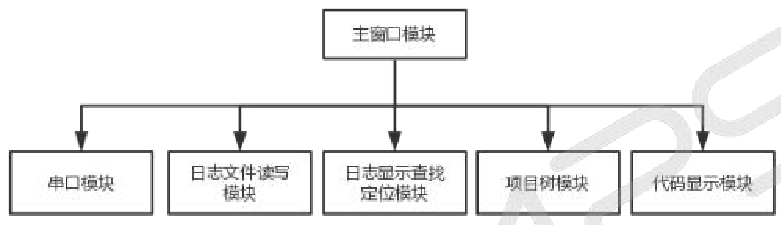
\includegraphics[width=1.0\textwidth]{./graphics/routonLog-system-structure.pdf}
\caption{调试信息分析工具结构图}\label{fig:日志分析工具结构图}
\end{figure}

\textbf{Log协议解析流程}
	日志界面的串口读取流程图如\autoref{fig:串口读取流程图} 所示,当用户打开串口后,主窗口中的串口读取函数会对串口中的数据进行非堵塞地读取,并按协议格式进行解析、显示和存盘。对于非协议格式的数据,则按照普通标准输出重定向过来的数据进行显示。此时在日志信息显示框中只会将信息显示在详细内容部分,日志级别、进程号、文件名、行号等内容均为空白。对于按照协议格式发送的信息,会按照信息的级别以不同的底色进行显示。
\begin{figure}[!h]
\centering
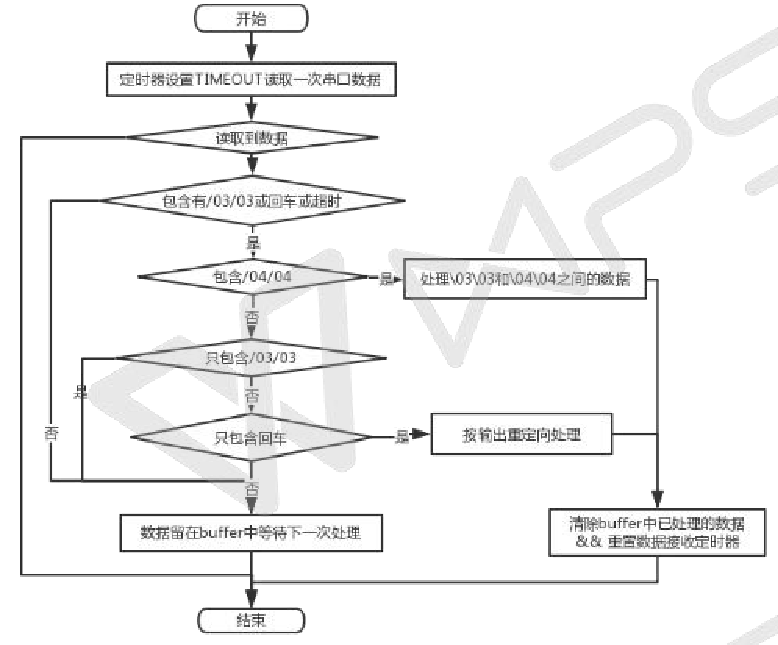
\includegraphics[width=1.0\textwidth]{./graphics/LogTTYRead.pdf}
\caption{协议解析流程图}\label{fig:串口读取流程图}
\end{figure}

\section{小结}
	本章首先介绍了我们的接口程序的设计分为了几个部分,每个部分的功能是什么,然后对我们的一个自定义的Log协议进行了介绍。最后分别在RTP模式和task模式下对接口进行了实现。	


\clearpage
\chapter{系统的功能测试}
\section{设备添加到系统管理表}
	查看当前的驱动程序是否已经添加到了系统当中,我们自定义的cp210xDevRead()、cp210xDevWrite()、cp210xDevOpen()、cp210xDevClose()、cp210xDevIoctl()是否已经和被注册到了IO子系统当中。只有成功的注册到了IO子系统当中,应用层的软件才能够通过标准接口open()、close()、read()、write()、ioctl()来对设备进行操作,完成设备的功能。
	首先通过iosDrvShow查看当前的cp210xDrvInit是否已经将驱动程序接口添加到了驱动程序列表当中,驱动加载前的系统设备表如\autoref{fig:iosDevShow}所示,驱动加载后的系统设备表如\autoref{fig:加载驱动后系统上的设备表}所示,显示了加载了驱动驱动之后多出来了一个驱动号为14的设备。由于两种情况下进行为不同的设备命名策略,所以显示出两个不一样的设备名。
\begin{figure}[!h]
\centering
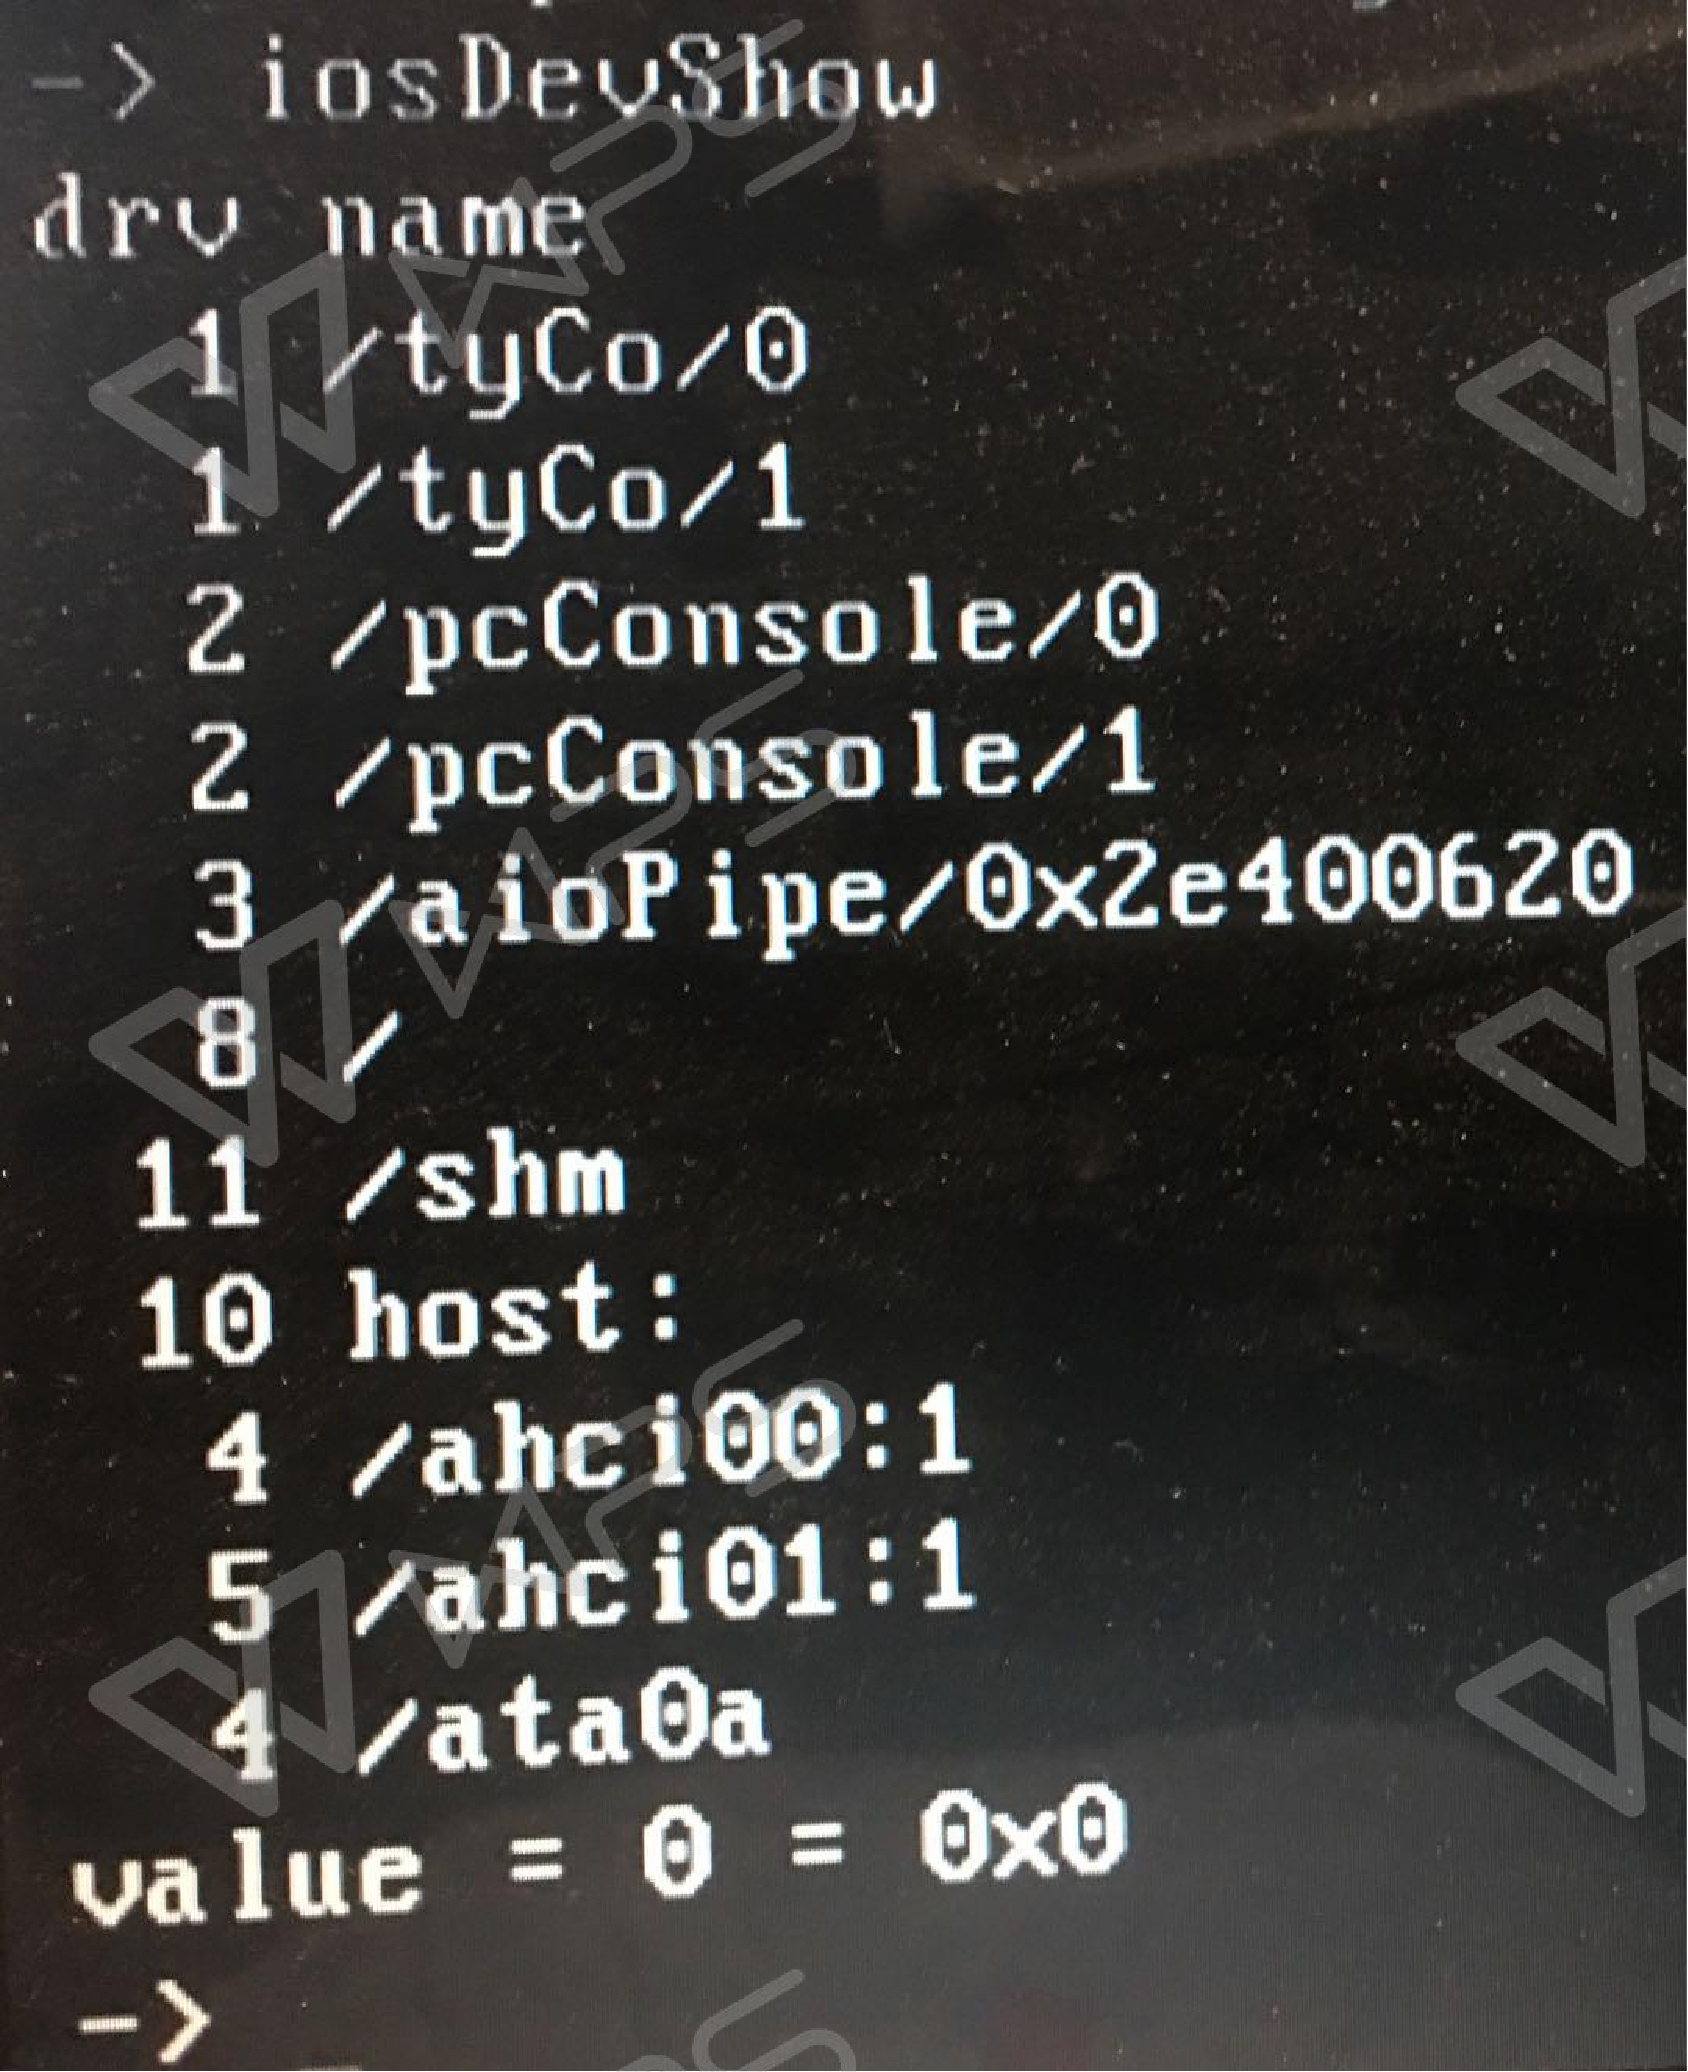
\includegraphics[width=0.7\textwidth ,height = 0.4\textwidth]{./graphics/iosDevShow.pdf}
\caption{驱动加载前系统设备表}\label{fig:iosDevShow}
\end{figure}

\begin{figure}[h]
\centering
  \begin{subfigure}[b]{0.4\textwidth}
  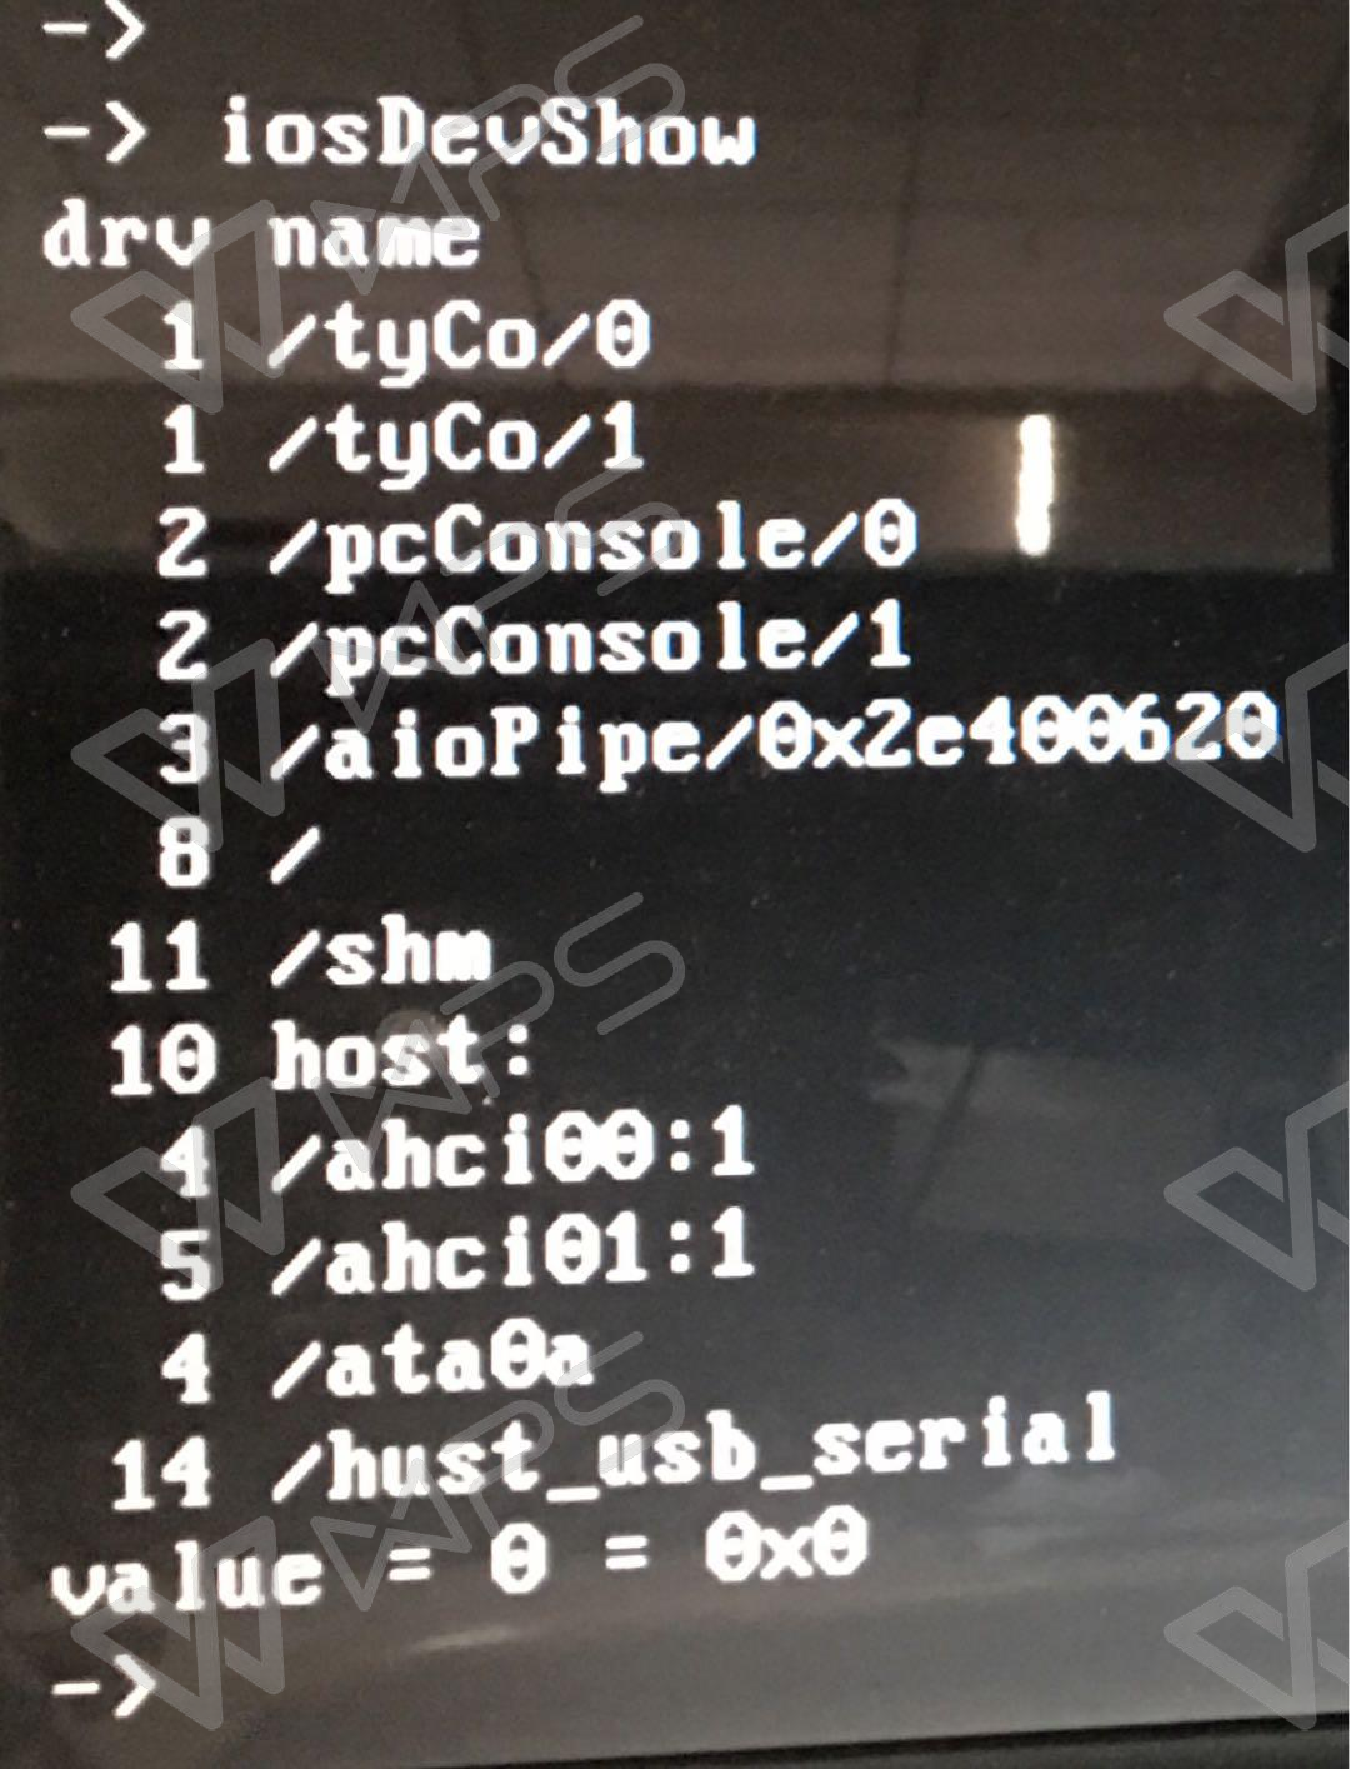
\includegraphics[width=\textwidth]{./graphics/iosDevShowS.pdf}
  \caption{单设备驱动}
  \end{subfigure}
  ~
  \begin{subfigure}[b]{0.4\textwidth}
  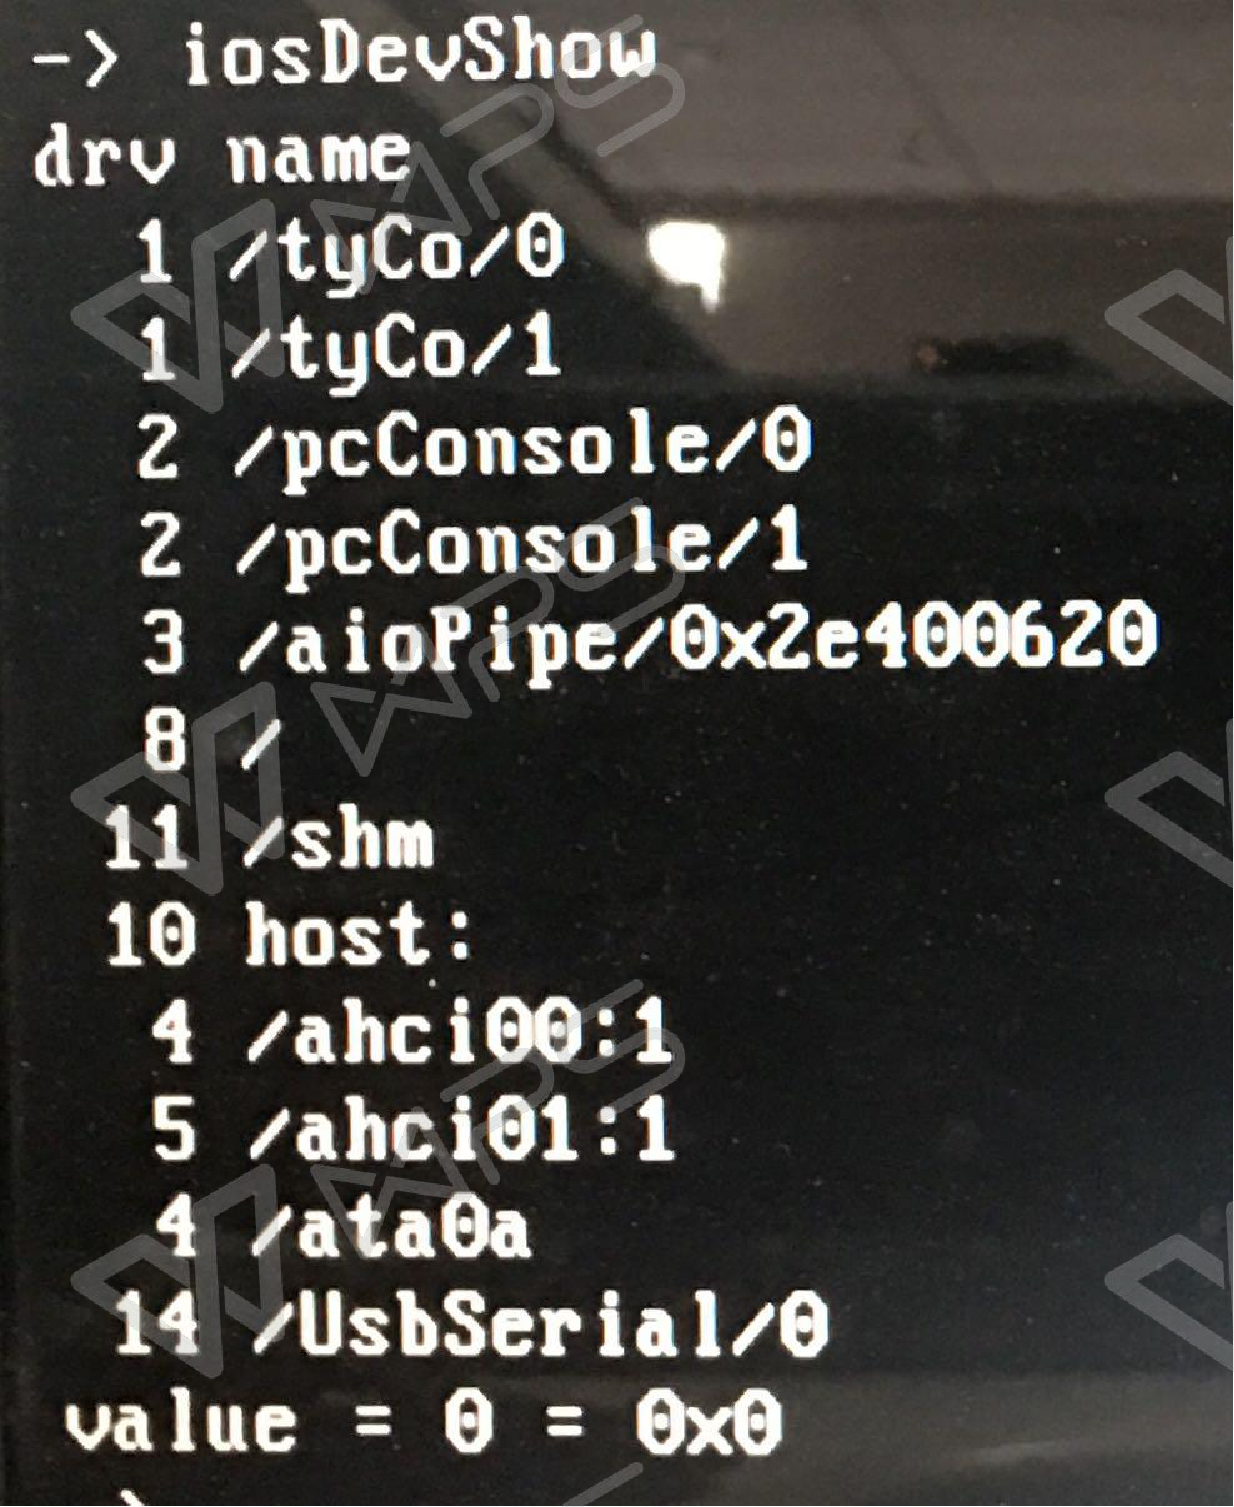
\includegraphics[width=\textwidth]{./graphics/iosDevShowM.pdf}
  \caption{多设备驱动}
  \end{subfigure}
\caption{驱动加载后系统设备表}\label{fig:加载驱动后系统上的设备表}
\end{figure}

\noindent 接下来查看设备驱动的接口是否已添加到驱动程序的列表当中,驱动加载前的系统驱动表如\autoref{fig:iosDrvShow}所示,驱动加载后的系统设备如\autoref{fig:加载驱动后系统上的驱动表}所示。
\begin{figure}[!h]
\centering
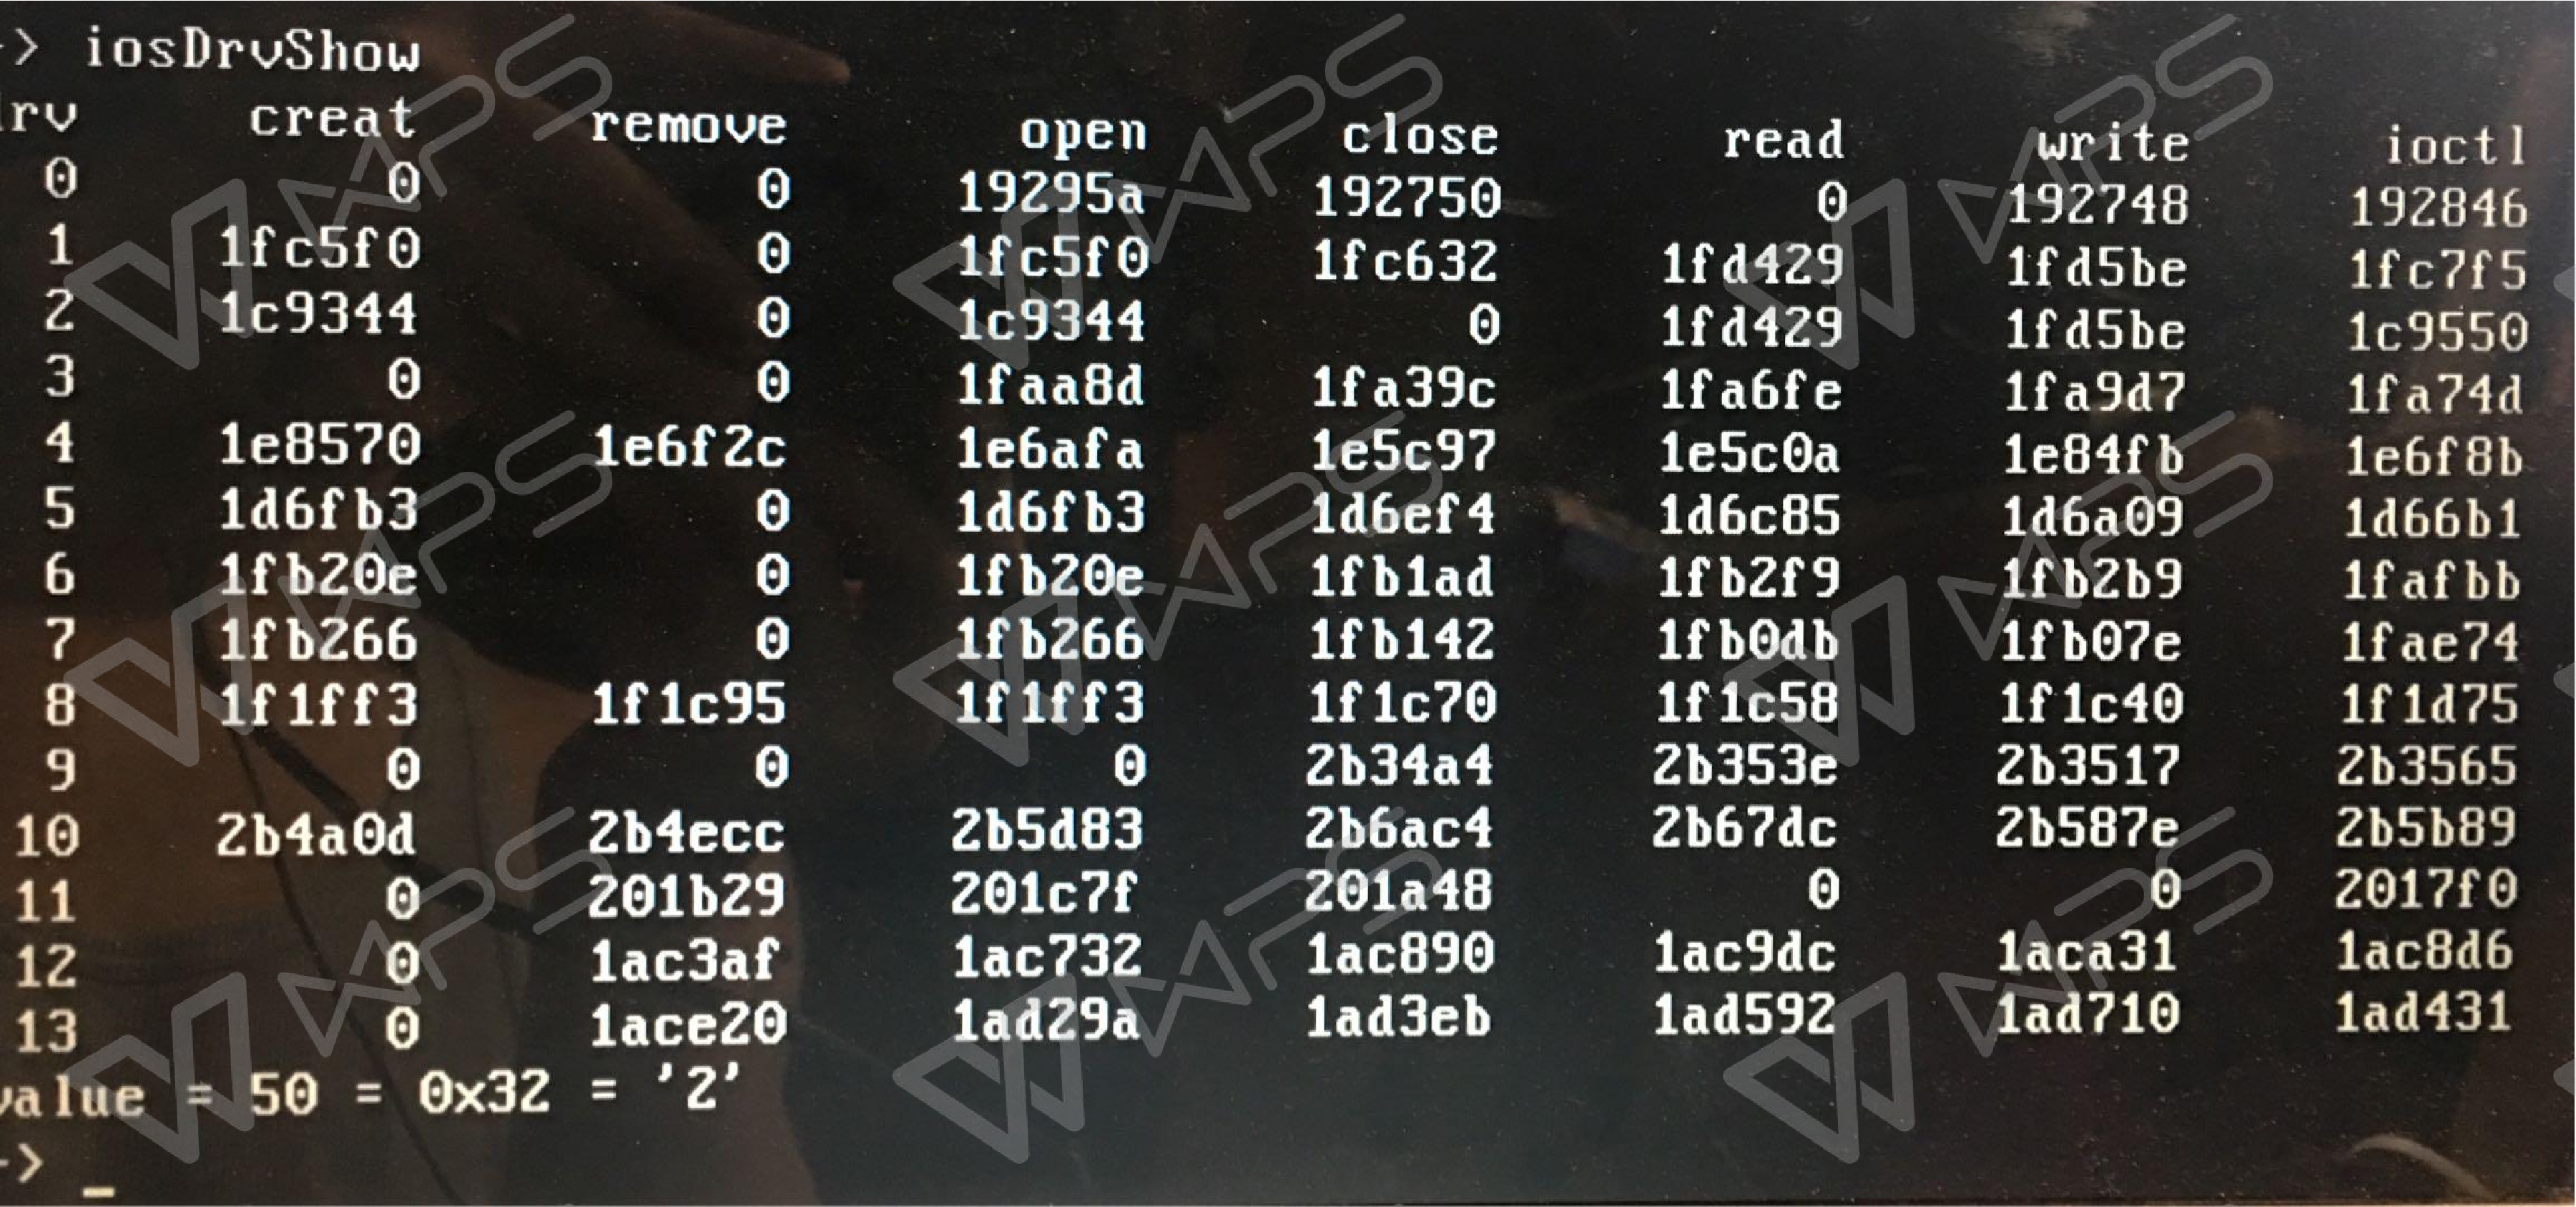
\includegraphics[width=.9\textwidth]{./graphics/iosDrvShow.pdf}
\caption{驱动加载前系统驱动表}\label{fig:iosDrvShow}
\end{figure}


\begin{figure}[h]
\centering
  \begin{subfigure}[b]{0.7\textwidth}
  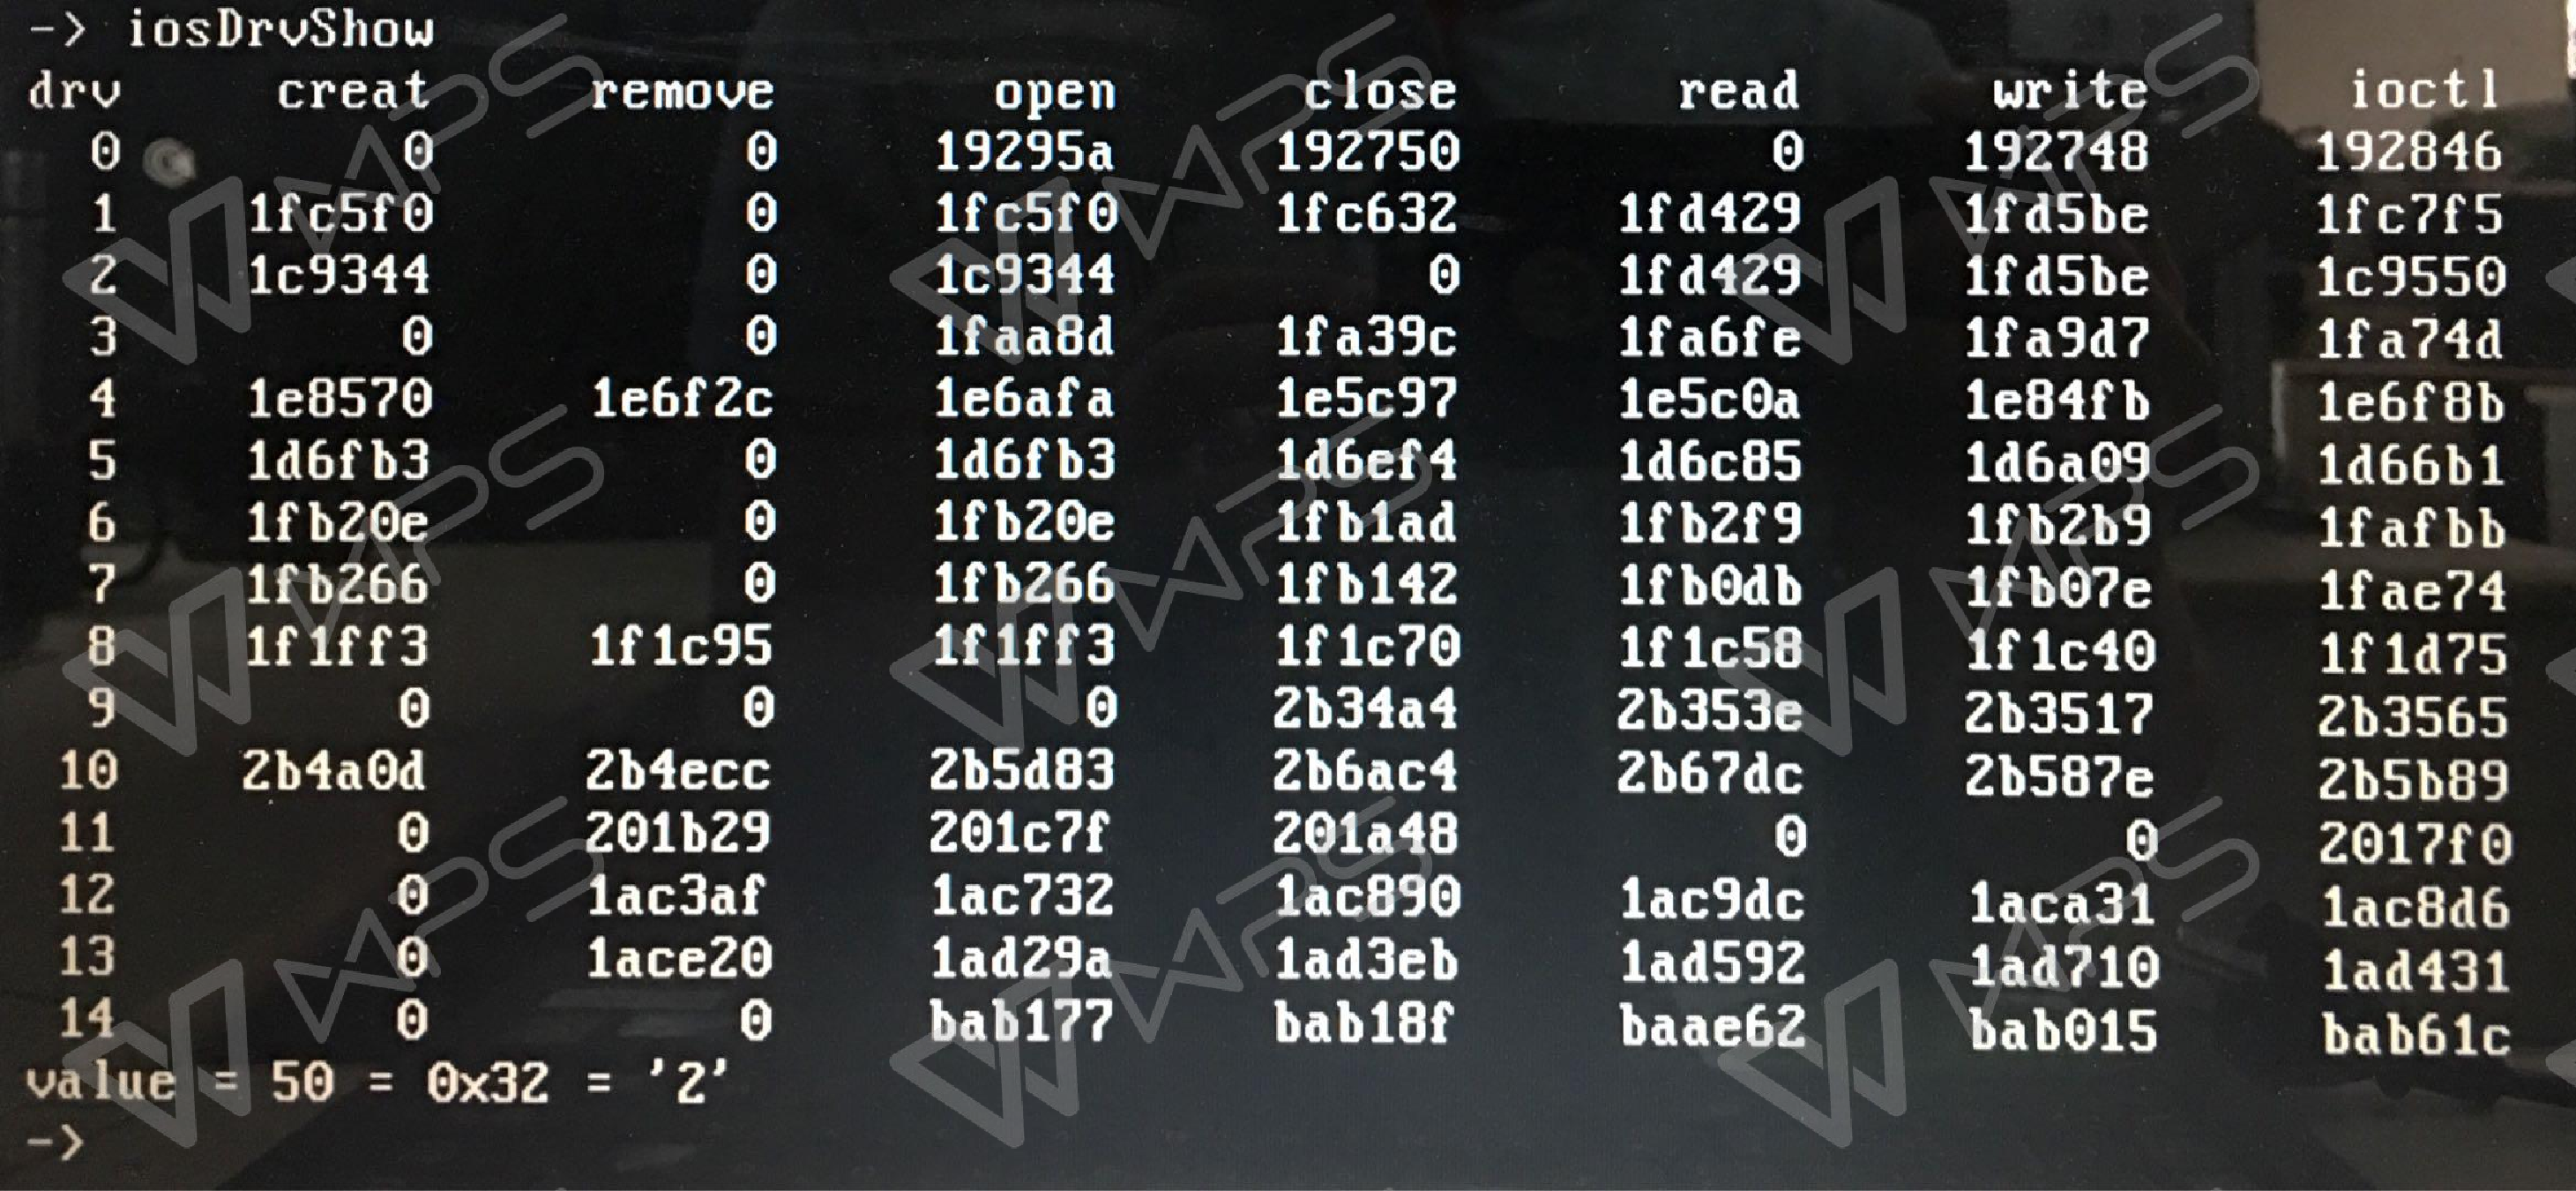
\includegraphics[width=\textwidth]{./graphics/iosDrvShowS.pdf}
  \caption{单设备驱动}
  \end{subfigure}
  ~
  \begin{subfigure}[b]{0.7\textwidth}
  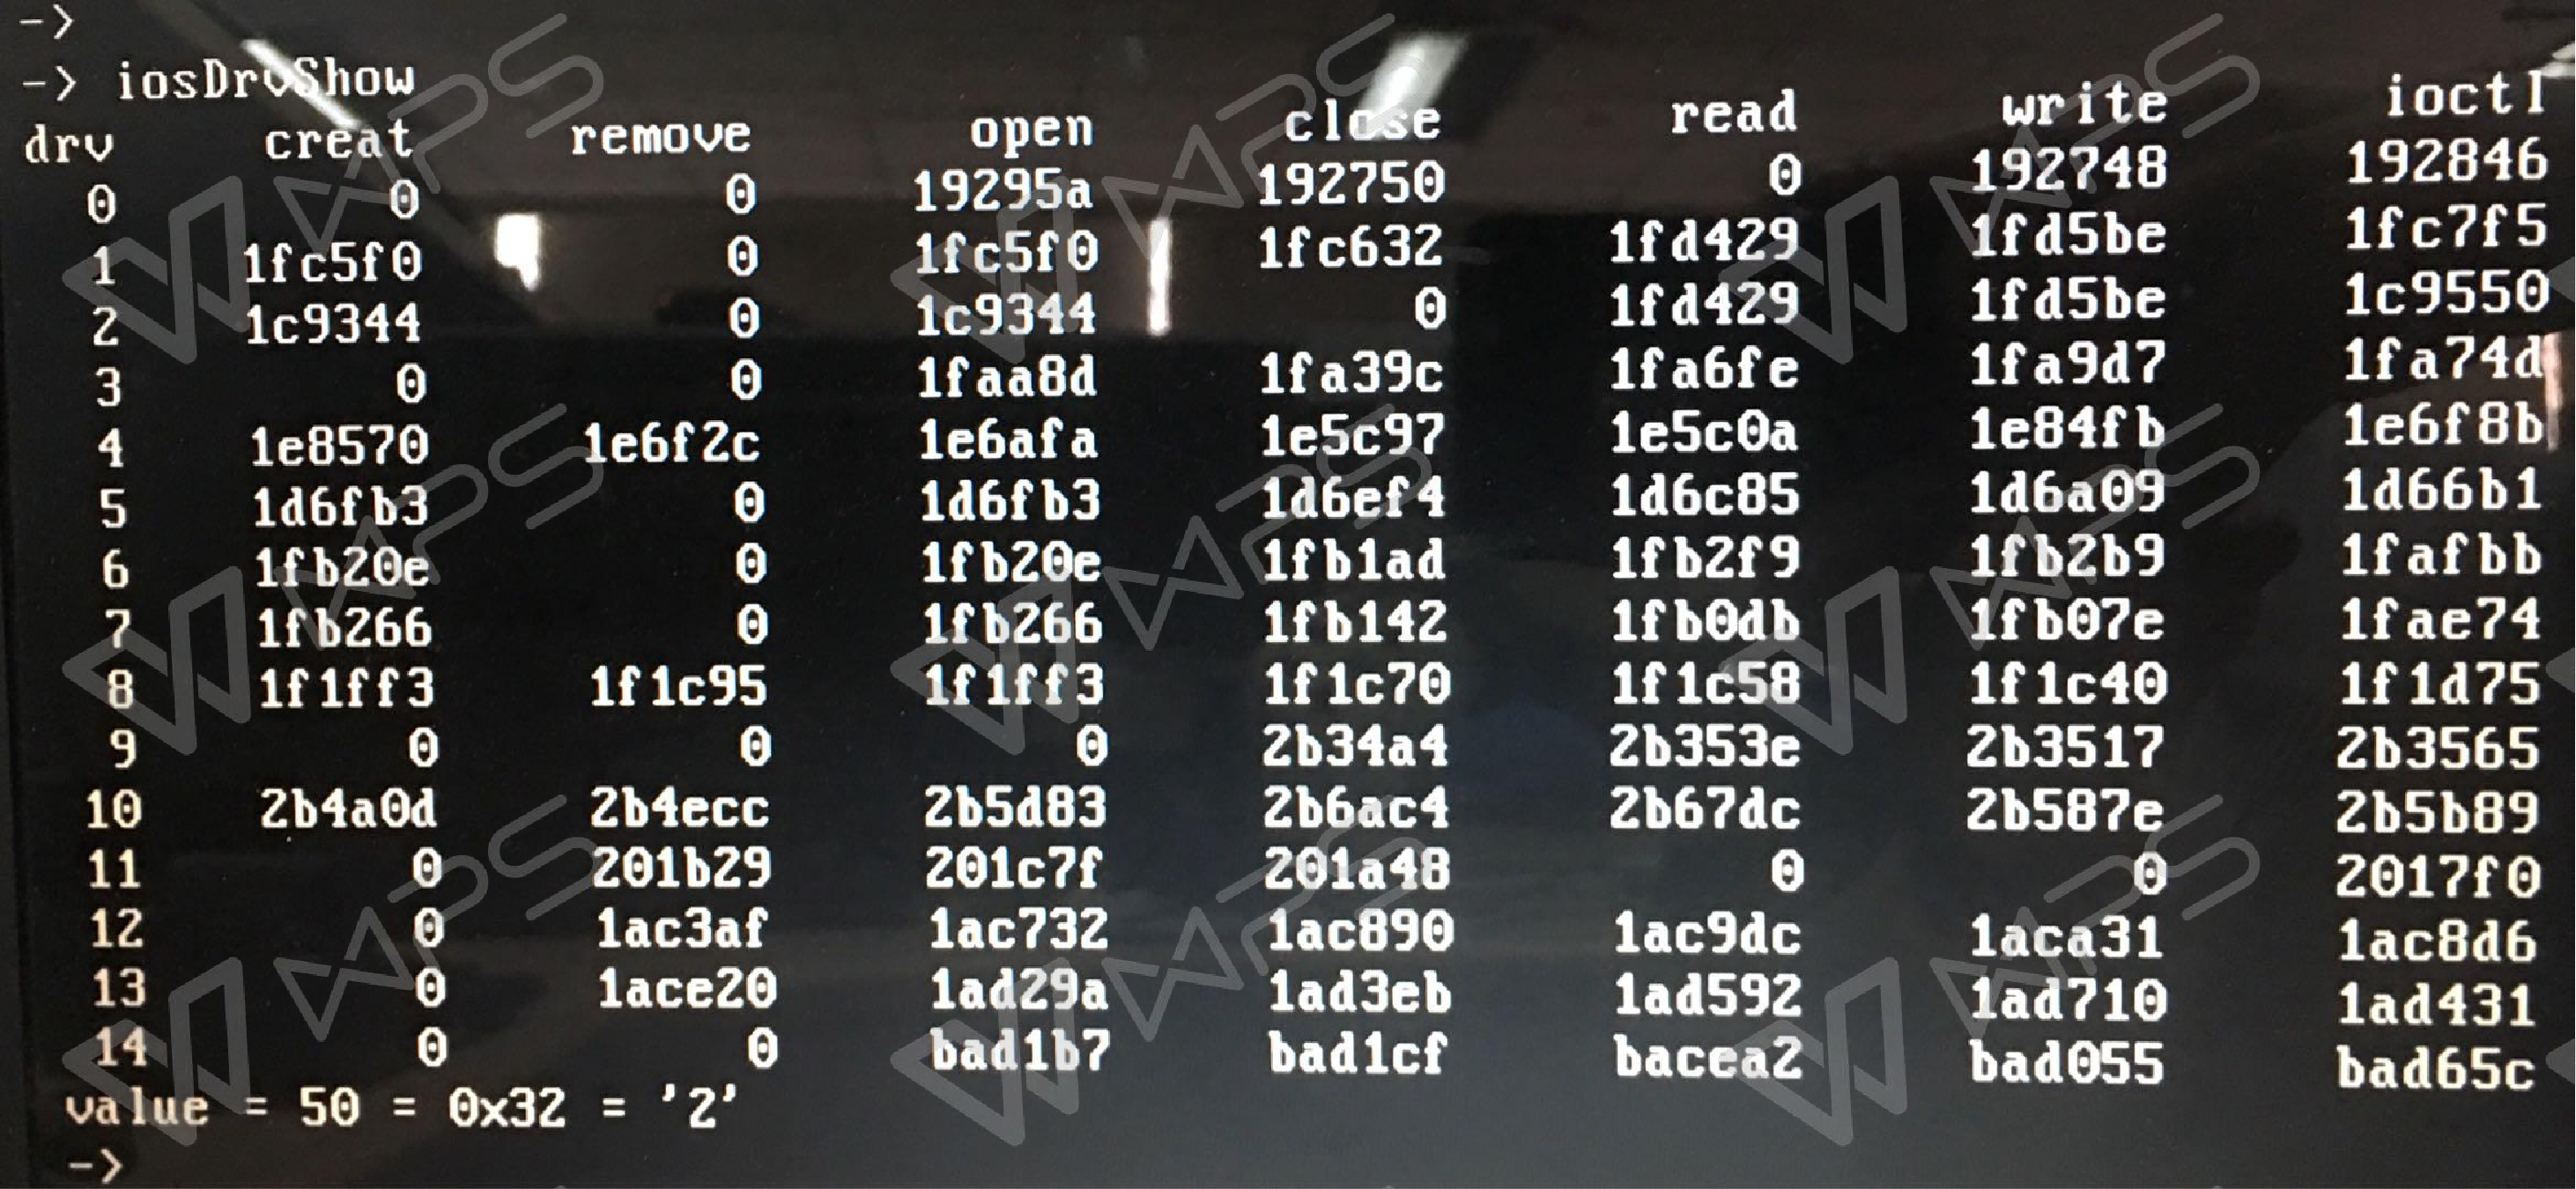
\includegraphics[width=\textwidth]{./graphics/iosDrvShowM.pdf}
  \caption{多设备驱动}
  \end{subfigure}
\caption{驱动加载系统驱动表}\label{fig:加载驱动后系统上的驱动表}
\end{figure}

\noindent 最后查看一下加载驱动之后是否能够正常的打开设备,打开设备之后应该会将其加入到系统文件描述符表当中,驱动加载前的文件描述符表如\autoref{fig:iosFdShow}所示,驱动加载后的文件描述符 表如\autoref{fig:加载驱动后系统上的文件描述符表}所示。
\begin{figure}[!h]
\centering
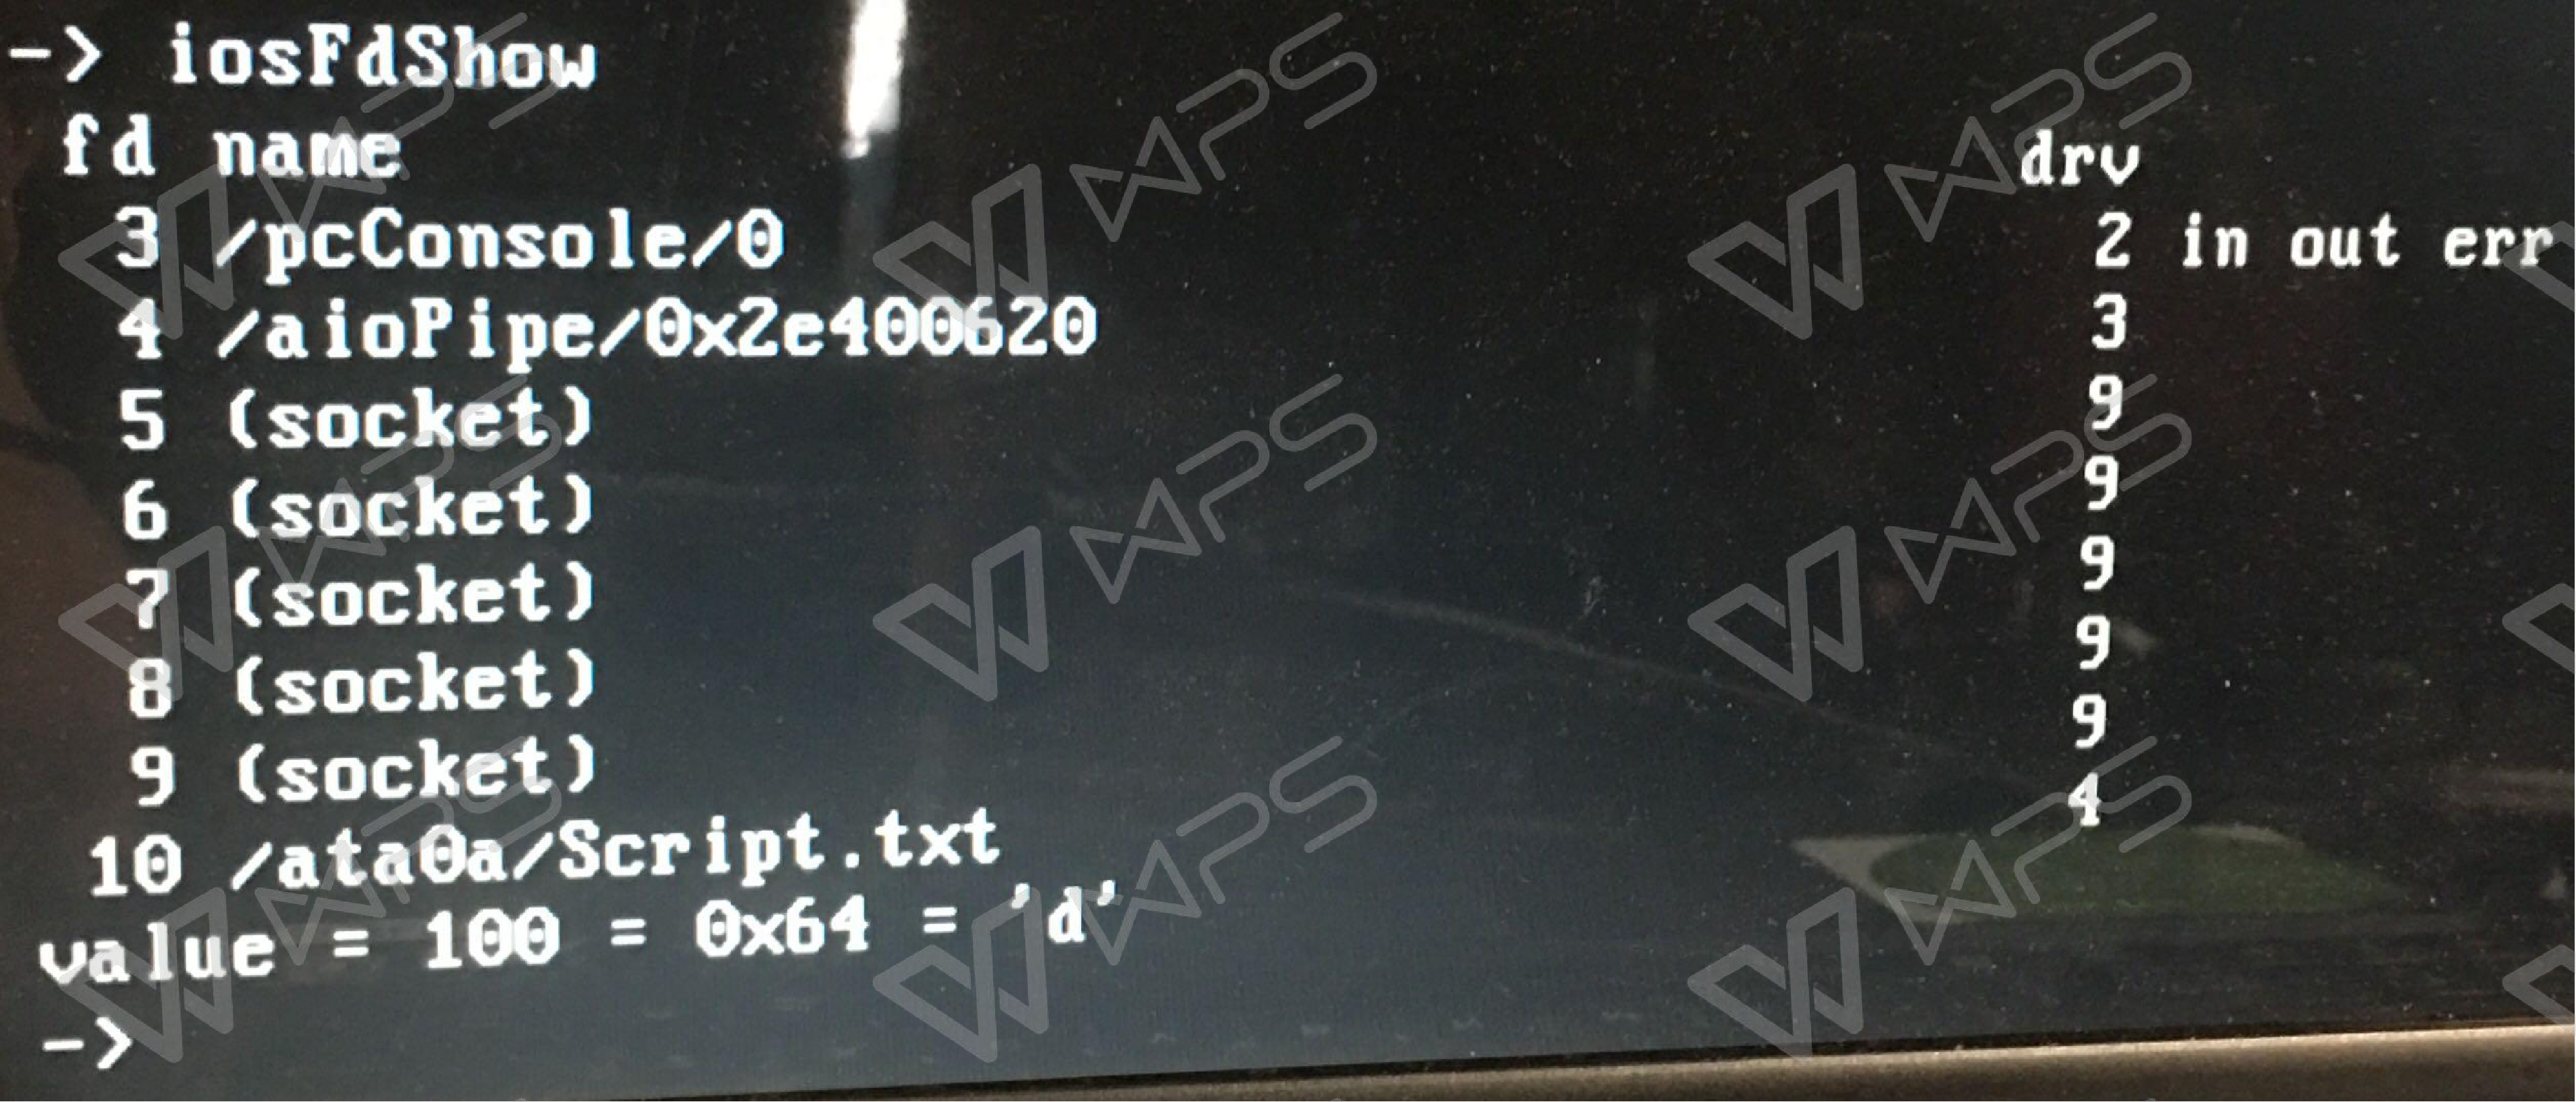
\includegraphics[width=.9\textwidth]{./graphics/iosFdShow.pdf}
\caption{当前系统上的文件描述符表}\label{fig:iosFdShow}
\end{figure}

\begin{figure}[h]
\centering
  \begin{subfigure}[b]{0.4\textwidth}
  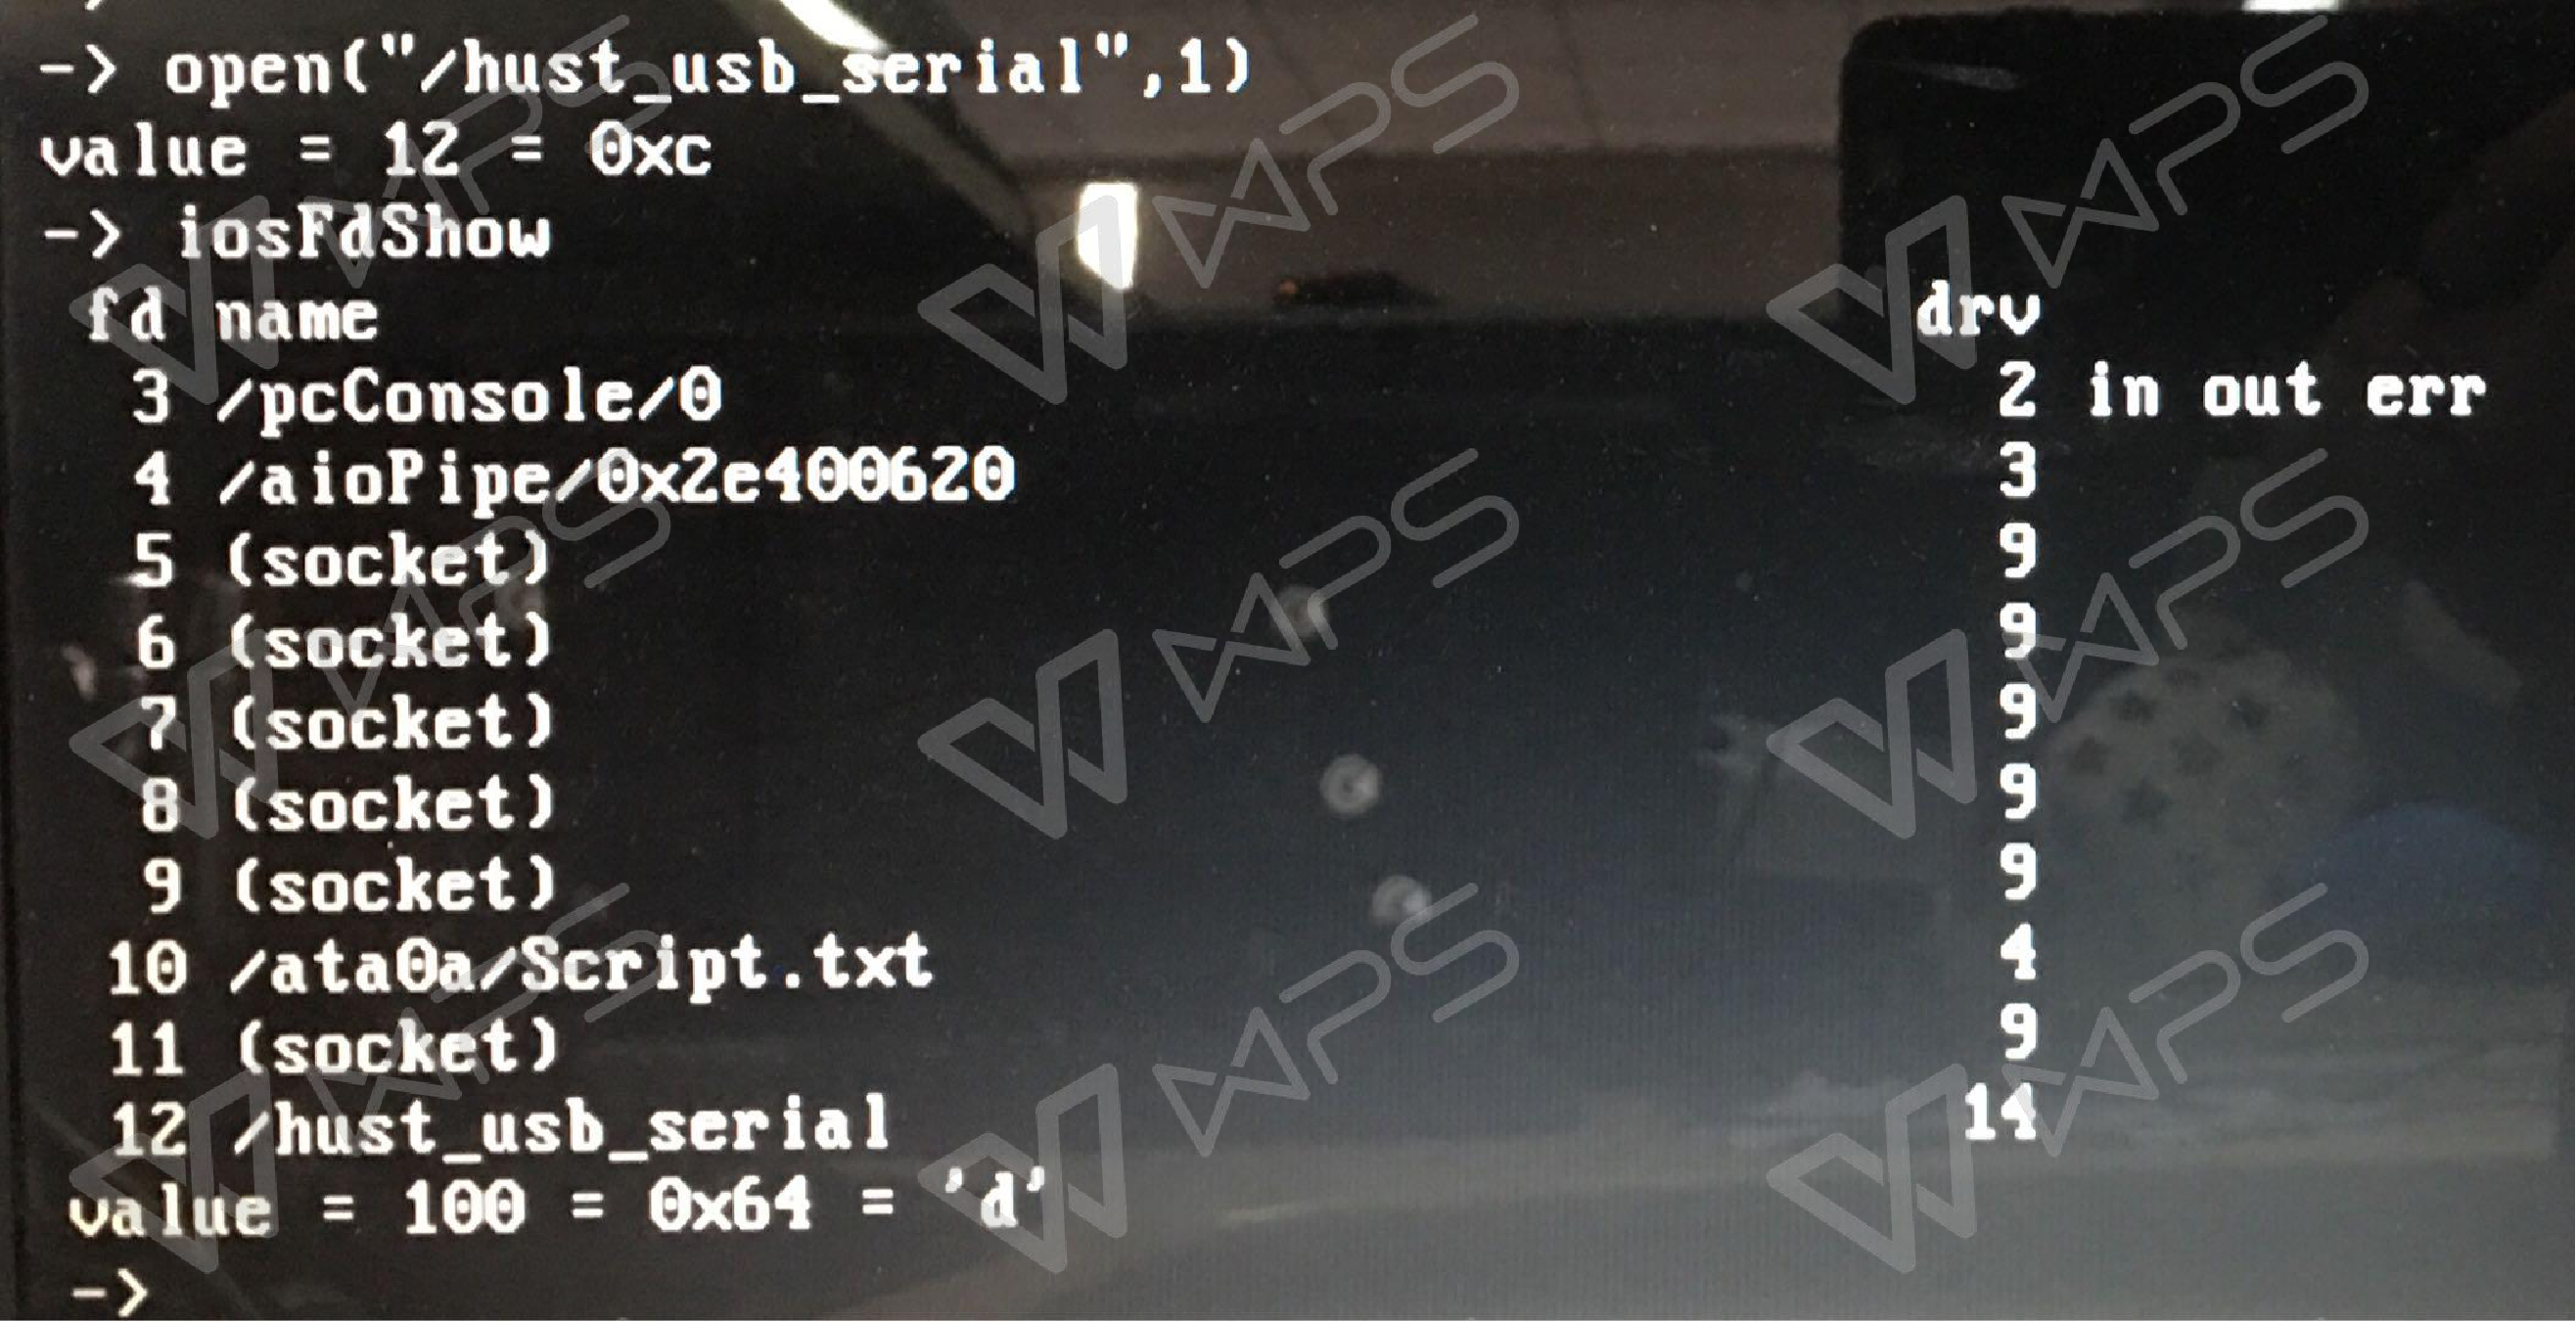
\includegraphics[width=\textwidth]{./graphics/iosFdShowS.pdf}
  \caption{单设备驱动}
  \end{subfigure}
  ~
  \begin{subfigure}[b]{0.4\textwidth}
  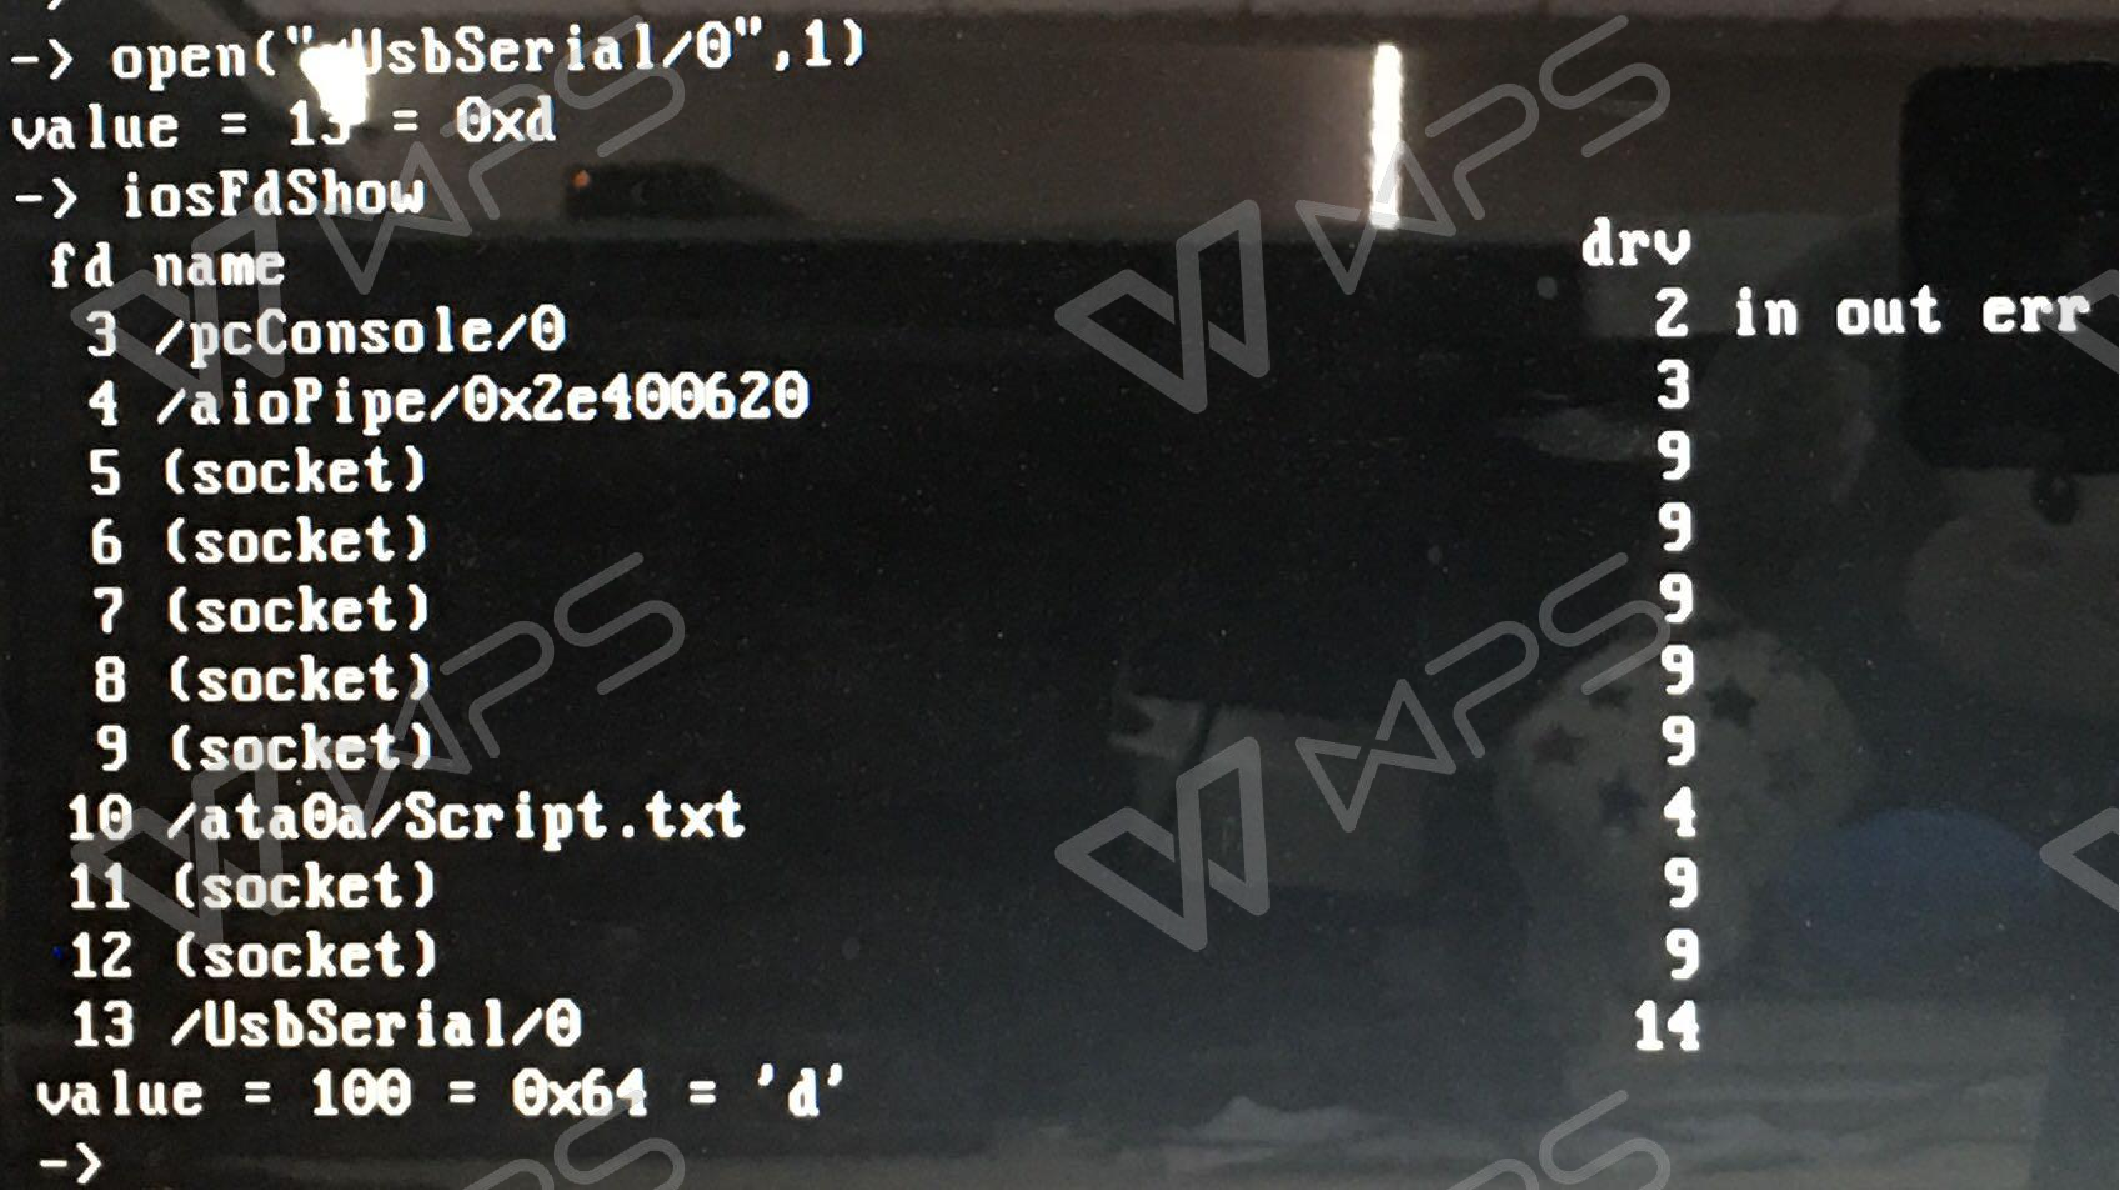
\includegraphics[width=\textwidth]{./graphics/iosFdShowM.pdf}
  \caption{多设备驱动}
  \end{subfigure}
\caption{加载驱动后系统上的文件名文件描述符表}\label{fig:加载驱动后系统上的文件描述符表}
\end{figure}

通过以上的验证说明了驱动程序已经被正常的安装,标准系统IO接口和驱动程序的IO子系统已经挂接成功。下一步将要进行进一步的功能测试,检测内部的各个IO接口是否能够正常的完成工作。
	
\section{驱动程序读写测试}
	由于VxWorks同时存在RTP模式和task模式,所以在这两种模式下都需要进行读写测试。
测试条件: 装有我们编写的USB口转串口驱动的VxWorks PC机,装有串口调试工具的windows PC机,USB转TTL模块在两台PC之间进行数据传输。

\subsection{RTP模式下的读写测试}
	测试报告如\autoref{tab:RTP模式下串口测试}所示。
\begin{table}[!h]
\centering
\begin{tabular}{|c|c|c|c|c|c|c|c|}
\hline
{\hei{波特率}} & {\hei{数据位}} & {\hei{数据位}} & {\hei{数据方向}} &{\hei{发送周期} & {\hei{发送次数}} &{\hei{信息数量}} &{\hei{正确率}} \\ 
\hline
{9600} & {8} & {0} & {读} & {0.1S/次} & {10000} & {500单词/次} & {100\%}\\
\hline
{9600} & {8} & {0} & {写} & {0.1S/次} & {10000} & {500单词/次} & {100\%}\\
\hline
{9600} & {8} & {0} & {读\& 写} & {0.1S/次} & {10000} & {500单词/次} & {100\%}\\
\hline 
{115200} & {8} & {0} & {读} & {0.1S/次} & {10000} & {500单词/次} & {100\%}\\
\hline
{115200} & {8} & {0} & {写} & {0.1S/次} & {10000} & {500单词/次} & {100\%}\\
\hline
{115200} & {8} & {0} & {读\& 写} & {0.1S/次} & {10000} & {500单词/次} & {100\%}\\
\hline
{921600} & {8} & {0} & {读} & {0.1S/次} & {10000} & {500单词/次} & {99.8\%}\\
\hline
{921600} & {8} & {0} & {写} & {0.1S/次} & {10000} & {500单词/次} & {100\%}\\
\hline
{921600} & {8} & {0} & {读\& 写} & {0.1S/次} & {10000} & {500单词/次} & {99.2\%}\\
\hline
\end{tabular}
\caption{RTP模式下串口测试}\label{tab:RTP模式下串口测试}
\end{table}


\subsection{task模式下的读写测试}
测试报告如\autoref{tab:task模式下串口测试}所示。
\begin{table}[!h]
\centering
\begin{tabular}{|c|c|c|c|c|c|c|c|}
\hline
{\hei{波特率}} & {\hei{数据位}} & {\hei{数据位}} & {\hei{数据方向}} &{\hei{发送周期} & {\hei{发送次数}} &{\hei{信息数量}} &{\hei{正确率}} \\ 
\hline
{9600} & {8} & {0} & {读} & {0.1S/次} & {10000} & {500单词/次} & {100\%}\\
\hline
{9600} & {8} & {0} & {写} & {0.1S/次} & {10000} & {500单词/次} & {100\%}\\
\hline
{9600} & {8} & {0} & {读\& 写} & {0.1S/次} & {10000} & {500单词/次} & {100\%}\\
\hline 
{115200} & {8} & {0} & {读} & {0.1S/次} & {10000} & {500单词/次} & {100\%}\\
\hline
{115200} & {8} & {0} & {写} & {0.1S/次} & {10000} & {500单词/次} & {100\%}\\
\hline
{115200} & {8} & {0} & {读\& 写} & {0.1S/次} & {10000} & {500单词/次} & {100\%}\\
\hline
{921600} & {8} & {0} & {读} & {0.1S/次} & {10000} & {500单词/次} & {100\%}\\
\hline
{921600} & {8} & {0} & {写} & {0.1S/次} & {10000} & {500单词/次} & {100\%}\\
\hline
{921600} & {8} & {0} & {读\& 写} & {0.1S/次} & {10000} & {500单词/次} & {99.6\%}\\
\hline
\end{tabular}
\caption{task模式下串口测试}\label{tab:task模式下串口测试}
\end{table}

在两种模式下都出现了在波特率较高的时候出现误码的现象,尤其是在同时进行数据的收发的时候出现误码的概率更大。会有很多的原因导致串口出现误码,例如干扰、接地不好、数据率过高、双方定时不一致等都会导致误码率的升高。

\section{应用程序接口测试}
\subsection{标准输出重定向测试}
测试条件:装有我们编写的USB口转串口驱动的VxWorks PC机,VxWorks下封装好的标准输出重定向接口以及USB转串口驱动, 装有串口调试工具的windows PC机,USB转TTL模块在两台PC之间进行数据传输。

测试同样分为RTP模式和task模式,因为在两种模式下实现重定向的机制并不一样。
1. task模式:
	在VxWorks中启动一个task程序,先调用标准输出重定向接口,查看其是否能够在程序中将标准输出重定向到串口.再定向回来,如此循环10000次,查看所有的输出是否显示在正确的终端上。测试结果如下:

\begin{table}[!h]
\centering
\begin{tabular}{|c|c|c|c|c|c|c|}
\hline
{\hei{波特率}} & {\hei{数据位}} & {\hei{数据位}} & {\hei{数据方向}} &{\hei{发送周期} & {\hei{发送次数}}  &{\hei{正确率}} \\ 
\hline
{9600} & {8} & {0} & {发送到本地终端} & {0.1S/次} & {10000}  & {100\%}\\
\hline
{9600} & {8} & {0} & {发送到远程终端} & {0.1S/次} & {10000}  & {100\%}\\
\hline
\end{tabular}
\caption{task模式重定向测试}\label{tab:task模式下重定向测试}
\end{table}
	

测试结果显示重定向接口能够在task模式下完美的完成重定向的功能。

2. RTP模式:
	
	RTP模式下的测试方式与在task模式下一样,在VxWorks中启动一个RTP程序,先调用标准输出重定向接口,查看其是否能够在程序中将标准输出重定向到串口.再定向回来,循环进行下去,查看输出是不是正确。
\begin{table}[!h]
\centering
\begin{tabular}{|c|c|c|c|c|c|c|}
\hline
{\hei{波特率}} & {\hei{数据位}} & {\hei{数据位}} & {\hei{数据方向}} &{\hei{发送周期} & {\hei{发送次数}}  &{\hei{正确率}} \\ 
\hline
{9600} & {8} & {0} & {发送到本地终端} & {0.1S/次} & {10000}  & {100\%}\\
\hline
{9600} & {8} & {0} & {发送到远程终端} & {0.1S/次} & {10000}  & {100\%}\\
\hline
\end{tabular}
\caption{RTP模式重定向测试}\label{tab:RTP模式下重定向测试}
\end{table}
注意这里的两个程序的区别,RTP模式下是main函数开始的,而task模式下是以内核模块的方式运行的。测试结果显示RTP模式下标准输出重定向也能够正常的完成工作,不会对系统造成混乱。

\subsection{Log日志接口测试}
	Log接口函数在RTP模式下和task模式下的实现方法是一样的,所以就不需要区分两种实现方式下的测试结果。我们以在RTP模式下的测试结果为例,测试完成的界面如\autoref{fig:RoutonLog}所示。在日志信息的显示框我们可以看到不同的颜色标识的不同级别的信息,包括我们自定义的协议的日志级别、进程号、进程名等信息都能正常的进行封装,并被正确的解析出来。
\begin{figure}[!h]
\centering
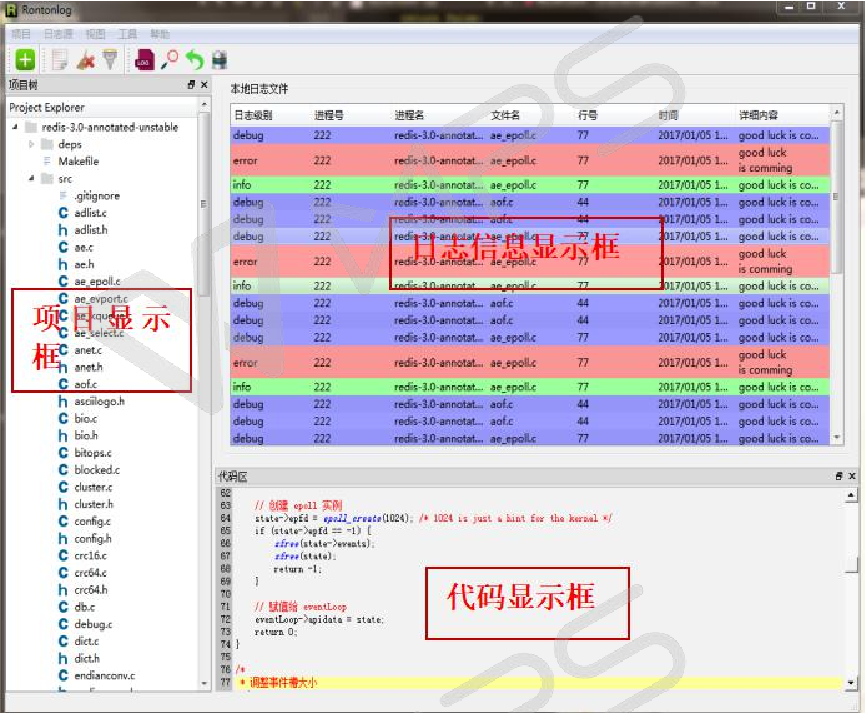
\includegraphics[width=1.0\textwidth]{./graphics/routonLogRun.pdf}
\caption{主机端日志分析工具测试界面}\label{fig:RoutonLog}
\end{figure}

测试报告如\autoref{tab:Log接口测试}所示。
\begin{table}[!h]
\centering
\begin{tabular}{|c|c|c|c|c|c|c|}
\hline
{\hei{波特率}} & {\hei{数据位}} & {\hei{数据位}} & {\hei{数据方向}}  & {\hei{发送次数}} &{\hei{信息类型}} &{\hei{正确率}} \\ 
\hline
{115200} & {8} & {0} & {写}  & {1000} & {LogE()} & {100\%}\\
\hline
{115200} & {8} & {0} & {写}  & {1000} & {LogW()} & {100\%}\\
\hline
{115200} & {8} & {0} & {写}  & {1000} & {LogI()} & {100\%}\\
\hline
{921600} & {8} & {0} & {写}  & {1000} & {LogO()} & {100\%}\\
\hline
{921600} & {8} & {0} & {写}  & {1000} & {LogD()} & {100\%}\\
\hline
\end{tabular}
\caption{Log接口测试}\label{tab:Log接口测试}
\end{table}

	需要注意的是上述的测试数据的是在1000次的循环内依次发送LogE、LogW、LogI、LogO、LogD的信息测试出来的,并不是每个级别的信息单独一个程序发送的。
	
	
\section{小结}
	本章对我们的驱动程序进行了一个整体的功能测试和各个部分的功能测试,查看系统的各个部分是否能够正常的工作 以及 整个系统的能够正常工作,是否能够达到设计的要求。通过测试结果我们可以看到系统已经基本达到了了本次的设计要求。各个模块都能够正常、稳定的运行。

\clearpage
\chapter{总结与展望}

	USB是一种新兴的外围接口标准,由于它众多的优良特性,且在现代PC中广泛使用,已经逐渐替代了其他的接口标准。本文选择了使用在VxWorks下使用USB口转串口的技术为基础,来实现一个调试通道。USB口转串口的硬件实现选择了目前市场上通用的CP2102芯片,因为芯片有良好的说明文档,并有大量的社区支持,对于驱动程序的编写更加方便。基于这个芯片我们在VxWorks上实现了一个针对该芯片的USB口转串口驱动。
	
	在本次的研究和开发的过程中,掌握了大量的关于USB接口和串口的相关知识,让我深深的体会到了USB驱动分层设计的好处与便利。要开发一个USB协议栈需要有很强的理论基础,明白各个层次之间的关系,上层应用程序与设备驱动之间的通信原理等。本次的设计是基于VxWorks操作系统之下的,之前从未接触过这类强实时性的嵌入式系统。在本次的开发过程中不断学习VxWorks系统的同时,也积累了大量的VxWorks下开发项目的实际经验。

	通过本次的项目我了解到了VxWorks的强大之处,其作为一个高性能的实时操作系统,成功的应用于很多大型的高尖端项目当中。在本次的发开过程当中我也只是学习到了VxWorks的冰山一角,对于其系统理论和实际应用的掌握还不全面。同时感受到了USB功能的强大和开发难度之大。USB凭借其优异的性能一定会成为更多外设的通用标准,同时	
用户也会对USB的带宽、据传输速率提出越来越高的要求,因此以后的USB技术肯定会更加的强大和完善,随着USB OTG、type C等标准的颁布,USB的应用领域和实用场景进一步得到强化。
	
	至此,本次设计的调试通道的功能已经基本实现,能够满足实际的应用中的需求。由于时间和能力有限,对于本次的调试通道的设计还有很多的不足之处,对于VxWorks下的USB口转串口的驱动程序部分还有很多的可以改进、完善的部分。例如在本系统中没有完成对设备的流控的设置,因为串口的传输速率有限,远远小于USB口的传输速率,使得串口速率成为了调试通道中传输速率的瓶颈部分,也许可以选择更好的数据传输方式来设计此通道。 
	
% backmatter用于表示论文的正文结束
\backmatter

%ack 环境用于致谢页面
\begin{ack}
\indent 转眼两年的研究生生活就要结束了,在此要感谢在这两年的学习生活当中教导我的老师和陪伴我一齐成长的同学,是他们陪伴着我在科研的路上一直奋斗,他们不断地激励着我、鼓励着我前进。
同时还要感谢论文的评阅人员,谢谢你们为我研究生生涯进行最后的把关、检验工作。


\noindent 本此的调试通道的设计工作能够顺利完成,还要特别感谢我的导师张杰老师,张老师从论文选题,构思到最后定稿的每个环节都一直给予我意见、指引与教导,在整个研究生生涯当中张老师都非常严格的要求我,这让我在研究生期间学习到了更多的知识。
也是在张老师的指导和帮助下,我才能够克服各种困难,突破一个又一个的技术难题,最终完成该调试通道的设计,使我得以最终完成毕业论文设计!
\end{ack}

% bibliography用于生成参考文献。
\nocite{*}
% \bibliographystyle{plain}
\bibliography{ref/myref.bib}


\end{document}

\endinput
%%
%% End of file `hustthesis-zh-example.tex'.
